%  Kandidate prosimo, da nam posredujejo predloge za izbolj''save tega vzorca 
%  na elektronski naslov Fizikalne knji''znice: fiz.knjiz@fmf.uni-lj.si.
%---------------------------------------------------------------------------------------
%        METAPODATKI
%--------------------------------------------------------------------------------------

\begin{filecontents*}{\jobname.xmpdata}
\Title{Naslov doktorske disertacije v angleškem jeziku}
\Author{Klemen Čotar}
\Keywords{disertacije\sep navodila}
\Subject{Physics}
\end{filecontents*}

%--------------------------------------------------------------------------------------

\documentclass[longbibliography,english,a4paper,12pt]{book}

\usepackage[english]{babel}    
\usepackage[utf8]{inputenc}
\usepackage{amsfonts}
\usepackage[T1]{fontenc}
\usepackage[pdftex]{graphicx}
\usepackage{fancyhdr}
\usepackage[sort, numbers]{natbib}
\usepackage{acro}

%--------------------------------------------------------------------------------------
%      DEFINICIJA AKRONIMOV
%--------------------------------------------------------------------------------------


\DeclareAcronym{FMF}{
  short            = FMF,
  long             = Fakulteta za matematiko in fiziko,
  class		= abbrev
  }

  
%-----------------------------------------------------------------------------------
%     PDF/A
%----------------------------------------------------------------------------------

\usepackage{xmpincl}
%\usepackage[a-1b]{pdfx} 

%------------------------------------------------------------------------------------  

\usepackage{filecontents}
\usepackage{hyperref}
\usepackage{url}
\usepackage[a4paper,inner=3.5cm,outer=2.5cm,top=2.5cm,bottom=2.5cm,pdftex]{geometry}
\usepackage[titletoc,title]{appendix}
\usepackage{epstopdf}
\usepackage{makeidx}
\pagestyle{fancy}
\setlength{\headheight}{15pt}
\usepackage{enumitem}
\usepackage{underscore}
\usepackage{tocloft}
\renewcommand{\cftpartleader}{\cftdotfill{\cftdotsep}} 
\renewcommand{\cftchapleader}{\cftdotfill{\cftdotsep}} 

\makeindex

\def\epsfg#1#2{\epsfig{file=#1.eps,width=#2}}
\def\legendamp#1#2{\vbox{\hsize=#1\caption{\small #2}}}

\setcounter{topnumber}{4}
\setcounter{bottomnumber}{4}
\setcounter{totalnumber}{5}
\renewcommand{\topfraction}{0.99}
\renewcommand{\bottomfraction}{0.99}
\renewcommand{\textfraction}{0.0}
\setlength{\tabcolsep}{10pt}
\renewcommand{\arraystretch}{1.5}

\def\bi#1{\hbox{\boldmath{$#1$}}}
\let\oldvec\vec
\def\vec#1{\mbox{\boldmath$#1$}}
\def\pol{{\textstyle{1\over2}}}
\def\svec#1{\mbox{{\scriptsize \boldmath$#1$}}}

%----------------------------------------------------------------------------------------
%    SUMNIKI
%----------------------------------------------------------------------------------------
%  Za pisanje sumnikov imamo tri moznosti:
%   --- vnasamo jih neposredno v kodnem sistemu UTF-8 (priporocljivo)
%   --- pisemo jih z latexovim ukazom, ki je namenjen natanko temu,
%       in sicer kot \v{c}, \v{s}, \v{z}, \v{C}, \v{S}, v{\Z} ali
%       malo manj pregledno kot \v c, \v s, \v z, \v C, \v S, \v Z,


%------------------------------------------------------------------------------------------
%   PRIPOROCILO
%
%  V primeru, da je besedilna datoteka prevelika za pregledno urejanje,
%  priporocamo, da vsebino razdelite na posamezna poglavja, ki jih v glavni
%  dokument vkljucite z ukazom \input{naslov_poglavja}.
%
%------------------------------------------------------------------------------------------

\begin{document}

%-----------------------------------------------------------------------------------------
%       NASLOVNA STRAN V ANGLESKEM JEZIKU
%----------------------------------------------------------------------------------------

\pagestyle{empty}
\begin{center}

{\large UNIVERSITY OF LJUBLJANA\\
FACULTY OF MATHEMATICS AND PHYSICS\\
DEPARTMENT OF PHYSICS\\}

\vspace{4cm}

{\Large Klemen Čotar\\}

\vspace{10mm}

{\bf \Large NASLOV DOKTORSKE DISERTACIJE V ANGLEŠKEM JEZIKU}\\
\vspace{5mm}
{\sc Doctoral thesis}\\

\vfill

{\large ADVISER: prof. dr. Tomaž Zwitter\\

\vspace{2cm}
Ljubljana, 2020}

\end{center}

%------------------------------------------------------------------------------------------------
%       NASLOVNA STRAN V SLOVENSKEM JEZIKU
%-----------------------------------------------------------------------------------------------

\cleardoublepage
\begin{center}

{\large UNIVERZA V LJUBLJANI\\
FAKULTETA ZA MATEMATIKO IN FIZIKO\\
ODDELEK ZA FIZIKO\\}

\vspace{4cm}

{\Large Klemen Čotar\\}

\vspace{10mm}

{\bf \Large NASLOV DOKTORSKE DISERTACIJE V SLOVENSKEM JEZIKU}\\
\vspace{5mm}
{\sc Doktorska disertacija}\\

\vfill

{\large MENTOR: prof. dr. Tomaž Zwitter\\

\vspace{2cm}
Ljubljana, 2020}

\end{center}
%------------------------------------------------------------------------------------------------
%        ZAHVALA (NEOBVEZNO)
%------------------------------------------------------------------------------------------------

\cleardoublepage
\mbox{}
\vfill
\foreignlanguage{slovene}{
{\Large \bf Zahvala}
\vspace{1cm}\\
Na tem mestu zapišite, komu se zahvaljujete za pomoč pri nastanku doktorske disertacije.
}

%-----------------------------------------------------------------------------------------------
%         IZVLECEK
%----------------------------------------------------------------------------------------------

\cleardoublepage
\foreignlanguage{slovene}{  % slovenski delilni vzorci
\begin{center}
{\bf Naslov v slovenskem jeziku}\\[3mm]
{\sc  Izvleček}
\end{center}
\vspace{10mm}
Kratek izvleček v slovenskem jeziku, do 300 besed.\\[10mm]
{\bf Ključne besede:}\\[3mm]
{\bf PACS:}
}


\cleardoublepage
\begin{center}
{\bf Naslov v angleškem jeziku}\\[3mm]
{\sc  Abstract}
\end{center}
\vspace{10mm}
Kratek izvleček v angleškem jeziku, do 300 besed.\\[10mm]
{\bf Keywords:}\\[3mm]
{\bf PACS:}

%---------------------------------------------------------------------------------------------------
%    KAZALO
%---------------------------------------------------------------------------------------------------

\cleardoublepage
\tableofcontents

%--------------------------------------------------------------------------------------------------
%        SEZNAM SLIK (NEOBVEZNO)
%---------------------------------------------------------------------------------------------------

%\cleardoublepage\phantomsection
%\renewcommand\listfigurename{List of figures}
%\addcontentsline{toc}{chapter}{\listfigurename}
%\listoffigures

%---------------------------------------------------------------------------------------------------
%        SEZNAM TABEL (NEOBVEZNO)
%---------------------------------------------------------------------------------------------------

%\cleardoublepage\phantomsection
%\renewcommand\listtablename{List of tables}
%\addcontentsline{toc}{chapter}{\listtablename}
%\listoftables

%--------------------------------------------------------------------------------------------------
%        SEZNAM KRATIC, SEZNAM SIMBOLOV (NEOBVEZNO)
%------------------------------------------------------------------------------------------------

%\cleardoublepage\phantomsection
%\chapter*{List of abbreviations and symbols}
%\renewcommand\listtablename{List of abbreviations and symbols}
%\addcontentsline{toc}{chapter}{\listtablename}
%\printacronyms[include-classes=abbrev, name=Abbreviations]
%\printacronyms[include-classes=nomencl, name=Symbols]
%\cleardoublepage

%--------------------------------------------------------------------------------------------------
%       OSREDNJI DEL
%--------------------------------------------------------------------------------------------------

\pagestyle{fancy}
\fancyhead[CE,RE]{}
\fancyhead[LO,CO]{}
\fancyhead[LE]{\textbf{\nouppercase{\leftmark}}}
\fancyhead[RO]{\textbf{\nouppercase{\rightmark}}}


\chapter{Introduction}
Primeri citiranj:

citealp: \citealp{APS}

citealp*: \citealp*{APS}

citealt: \citealt{APS}

citealt*: \citealt*{APS}

citeauthor: \citeauthor{APS}

citeauthor*: \citeauthor*{APS}

citefullauthor: \citefullauthor{APS}

citeauthor*: \citeauthor*{APS}

citenum: \citenum{APS}

citep: \citep{APS}

citet: \citet{APS}

citet*: \citet*{APS}

citeyear: \citeyear{APS}

citeyearpar: \citeyearpar{APS}

 % intro
Observational studies and simulations show that stars in our Galaxy were not formed at the same time, but at multiple epochs in different places of the Galaxy \cite{2001ApJ...554.1044C, 2017ARA&A..55...59N}. One of the youngest building blocks of the Galaxy are open stellar clusters whose stars formed from the same molecular cloud of material \cite{2003ARA&A..41...57L} and therefore retain some properties of the original cloud they were made from. Stellar properties of an individual star can be separated into a kinematic and chemical component. The first is describing the position and movement of a star in the Galaxy. The second gives information about its chemical composition and physical properties. During the evolution of the Galaxy, clusters that have a lower number of members and are therefore gravitationally loosely bound, slowly evaporate because of different effects such as gravitational dynamical friction and ejection of stars during close intra-cluster stellar interactions. The latter is a result of close gravitational interactions among members, where one of them can be ejected out of a cluster at high velocity \cite{2009MNRAS.396..570G, 2010MNRAS.402..105G, 2017MNRAS.470.3049R}. Such past members can on the sky be found even several degrees away from their main cluster body \cite{2007MNRAS.376L..29G, 2018MNRAS.473.4612K, 2019ApJ...884....6M}. The gravitational dynamical friction happens when a cluster moves trough regions of the Galaxy with a higher density of stars \cite{2010MNRAS.401.2753B}. During such event, the gravity of a cluster starts pulling seemingly fixed stars around it. Considering energy and momentum conservation law, we can conclude that a cluster will be slowed down for the same amount. This slowing subsequently changes the orbit of individual cluster members around the centre of the Galaxy. Small orbital changes lead to a gradual expansion of a cluster volume that can be tracked until its individual stars blend with a general stellar field population, making them unrecognizable as past cluster members. The most prominent transitional features we can observe are compact cluster tidal tails \cite{2019AA...627A...4R, 2019AJ....157..115Y, 2019AA...621L...3M, 2019arXiv191206657Z} and lose extended halos of evaporated stars. The halos can be observed as a slowly decreasing over-density \cite{2002A&A...385..471C, 2004A&A...427..485B, 2019AA...627A.119C} of stars far from a denser central cluster core.

% cluster ages
Born from the same molecular cloud, open clusters are therefore ideal tracers of formation, assembly and evolutionary history of their host galaxies. Being influenced by external and internal processes, their lifetime is limited from about $100$~Myr to a few Gyr for the densest structures \cite{1998A&A...337..363P, 2013MNRAS.434.2509M}. Studies have shown that the dissolution time of a cluster depends mainly on its total mass, its radius and its galactic environment (density of the stars around it and on its galactic path). Many papers have so far dealt with the question of determining the precise lifetime of stellar clusters before they completely dissipate into field population. The problem has been tackled using direct N-body simulations \cite{1998A&A...337..363P} where the movement of individual stars was traced, and from direct observational data \cite{1971Ap&SS..13..300W, 1988IAUS..126..393W, 2019MNRAS.487.2385M, 2019A&A...623A.108B} using isochrone fits. Age distribution of open clusters within a distance of $1$~kpc from the Sun shows a cluster median lifetime of $200$~Myr. Their broad range in ages gives us a possibility of observing them at different evolutionary stages \cite{2006BASI...34..153C, 2007A&A...468..139P} before they blend \cite{2001A&A...366..827B} into a field stellar population. On the other hand, such a short lifetime (in comparison with a lifetime of a Sun-like star) gives us a limited number of bounded clusters in the sky that can be studied at a given time.

% imf and mass segregation
The processes described above heavily depend on the mass of a cluster, its internal structure and mass distribution of its components. When star formation ceases, we are left with a wide range of stellar masses. Their distribution can be described by an initial mass function (IMF) \cite{1955ApJ...121..161S, 1986FCPh...11....1S, 2003PASP..115..763C} that appears invariant among clusters and even stars in the field \cite{2001MNRAS.322..231K}. The initial spatial distribution of stars in young clusters may reflect the structure of parental molecular cloud \cite{2015MNRAS.448.1847H}. In many stellar clusters, the brightest and most massive stars are concentrated towards the centre of a cluster, this state is usually attributed to mass segregation. Whether mass segregation occurs due to an evolutionary effect or it is of primordial origin is not yet entirely clear \cite{1998A&A...333..897R, 1998MNRAS.295..691B, 2002MNRAS.331..245D, 2003A&A...405..525B}. In the first case, massive stars are formed all around the cluster volume and eventually sink to its centre through the effect of two-body relaxations. In the second scenario, massive stars form preferentially in the central region of a cluster either by gas accretion due to their favourable location at the bottom of a gravitational potential well or through a coalescence process of less massive stars. The fact that mass segregation is also observed in young clusters might suggest that the second scenario is more likely that the evolutionary mass segregation, but the question is still under investigation \cite{2018MNRAS.473..849D}.

% binaries 
Similarly to the IMF, we can also define the initial binary population (IBP) of the observed sample of stars. Characterizing fraction of binaries in stellar clusters is of great importance for many fields of astrophysics. Since binaries are on average more massive than single stars, they are thought to be useful tracers of dynamical mass segregation \cite{2015arXiv151000099D}. Comparing observations with a theoretical model for the radial distribution of binary systems and their properties (mass and luminosity ratio, orbital period) distribution can be used to assess the dynamical state of a cluster \cite{1999NewA....4..495K}.

\section{Open clusters in the \G\ era}
\label{sec:open_clust_gaia}
Since \G\ Data Processing and Analysis Consortium (DPAC) centres responsible for analysis of the \G\ observations started publishing publicly available ready-to-use stellar properties, many new discovers and insights have been made. For the first time in history, we reliably know the position, distance, complete spatial velocity (proper motion and radial velocity) and luminosity for millions of bright and dim stars all across the observable sky. Their accuracy heavily depends on the source brightness. For example, published \G\ parallax uncertainties are in the range from $0.04$ to $0.7$~mas for the faintest sources. Similarly, radial velocities are precisely known in the range from 300~\ms to 3~\kms (further details are given in Section \ref{sec:gaia_data}).

One of the fields in astronomy that massively benefited from those new and improved measurements was a research of open stellar clusters.

% looking for clusters, unreliable detection
A traditional historical way to look for open stellar clusters was through counting stars as they are seen on the sky from Earths' location and finding over-densities in those counts \cite{1988AJ.....95..108L, 2014A&A...568A..51S}. To perform a more robust selection, members were additionally filtered based on their apparent distance from the cluster centre and their motion vectors \cite{2017A&A...601A..19G}. Using the latest second release of \G\ data \citep[DR2,][]{2018A&A...616A...1G}, we can go beyond that and build upon the results achieved by the methods mentioned above. Complete \G\ information on stellar distance, kinematics and photometric measurements enable us to go beyond simple methodologies, to unravel even the faintest and sparsest components of open clusters. So far, many works have been published trying to refine parameters, and membership information of long known open clusters \cite{2017A&A...601A..19G, 2018A&A...618A..93C, 2019A&A...627A..35C} and find new, less numerous or fainter clusters \cite{2019arXiv190904612B, 2019ApJS..245...32L, 2019JKAS...52..145S, 2019A&A...624A.126C, 2020arXiv200107122C}. Such thorough and the improved investigation uncovered that many of the clusters listed in modern catalogues, initially discovered as apparent stellar overdensities, are no more than chance alignments of stars and not true physically bound clusters \cite{1998A&A...340..402B, 2000A&A...357..145C, 2016AJ....152....7H, 2018MNRAS.480.5242K, 2020A&A...633A..99C}.

% starosti zvezd za kopice in field
Precisely determined open cluster membership also enables accurate age determination of a cluster and its stars \cite{2018ApJ...863...65C}. When observing stars in any random stellar field, it is notoriously hard to determine their ages as they remain unchanged for the majority of their lifetime. While it is possible to obtain precise age estimates for some specific classes of stars \cite{2010ARA&A..48..581S}, a uniform methodology does not exist for all. Age determination is much easier for stars in a cluster as they are all of a very similar age. Stellar evolution and its cycle are determined mainly by the initial mass of a star. Observing stars of different masses in a cluster reveals its evolutionary stage and consequently also its age by comparing them to theoretical evolutionary models. The latest \G\ data enabled researchers to compute stellar absolute magnitudes and colours that are commonly used in those comparisons \cite{2019MNRAS.487.2385M, 2019A&A...623A.108B, 2019A&A...631A.166K}.

% mass segregation
Another advantage of the newest \G\ dataset, with accurately determined distance to objects, is the possibility of determining the actual shape of a cluster, mass segregation of member stars and their gravitational potential from the first principles. Until recently that was possible only through n-body simulations \cite{1987MNRAS.224..193T, 2016MNRAS.456.3757S, 2018MNRAS.473..849D} that were compared with available observational datasets. For distant stellar associations, the distance error bars are still larger than a cluster itself, but improvements are expected when \G\ EDR3 will be released in the second half of the year 2020 or later. Internal cluster dynamics can in those cases be inferred using precisely determined radial velocities and proper motion vectors whose uncertainty is not affected by stellar distance, but their apparent brightness. Deviations (overtaking or lagging) from the mean cluster velocity can be therefore be used to assess in which direction, away from the mass centre, stars are moving. This velocity deviation consequently also indicates its position in a cluster. Reliable determination of stellar mass distribution in a cluster also depends on accurate classification of binary or higher multiplicity stars and their masses. By using pure \G\ information, they can be identified as stars with higher radial velocity uncertainty \cite{2018RNAAS...2b..20E}, by its temporal variation in future data releases \cite{2019AJ....158..155B}, using precise absolute magnitudes \cite{2018ApJ...857..114W, 2018A&A...616A..10G, 2019MNRAS.487.2474C} or by exploring astrometric uncertainties \cite{2020arXiv200305467B} that indicate movement of their combined photocentre. 

\section{Chemical tagging}
\label{sec:open_clustesr_tagging}
Majority of previously described works in Section \ref{sec:open_clust_gaia} relies on a complete 6D positional and kinematics information to discover clusters and their sub-structures. Advances in observational techniques and data analysis enables us to go beyond kinematics information and include a multidimensional chemical signature of stars -- the procedure known as chemical tagging \cite{2002ARA&A..40..487F, 2010ApJ...721..582B}. So far a blind chemical tagging (without kinematics) that would delineate between cluster and field stars has not yet been demonstrated with great success unless the observed structure has obviously different chemical composition \cite{2016ApJ...833..262H}. A trait that it is not common to open stellar clusters formed at about the same time \cite{2019A&A...629A..34G}, but to galactic components formed at vastly different epochs \cite{2018A&A...619A.125A} of Galaxy formation.

The measured chemical signature of a star gives us its composition in the outer-most layer, where it remains unchanged for young stars. Its composition is, therefore, a direct reflection of a medium from which it was built. Galaxy started evolving from dust made predominantly from hydrogen and helium which slowly got polluted by evolved stars during their final evolutionary stages. This gradual enrichment is nowadays observable as gradients of chemical abundances in radial and vertical directions of Galaxy. Internal gravitational mixing causes blending of those signatures as stars move to different orbits. Already complicated chemical structure of Galaxy is in some regions interrupted by newly created dense stellar structures -- open clusters -- which we would like to discover by the above-described procedure. Because of multiple gradual processes going on in Galaxy, the chemical tagging so far does not have clearly defined cuts to separate galactic components.

The latest research showed that many, even unexpected, observational and data reduction issues still have to be thoroughly investigated and resolved, especially if data from different surveys are to be combined \cite{2019ARA&A..57..571J}. Studies suggest that open clusters might not be as homogeneous as thought before \cite{2016ApJ...817...49B, 2018MNRAS.473.4612K}, and abundances show traits of stellar evolution \cite{2015A&A...577A..47B, 2017ApJ...840...99D, 2018MNRAS.478..425B}. On top of that, the main concerns of chemical tagging are abundance trends assumingly induced by spectral analysis \cite{2016ApJ...817...49B, 2019arXiv191208539C, 2020arXiv200103179B}. Observed trends depend on determined stellar physical parameters (i.e. \Teff\ and \vsin) and might be results of inadequate stellar models or actual stellar processes. To cope with this complexity and uncertainties, complex Bayesian models are being developed \cite{2016ApJ...817...49B, 2019ApJ...887...73C} in order to uncover and cluster abundance patterns. With this in mind, many work and validation still have to be done until large surveys are fully ready for blind chemical tagging experiments.

\section{Peculiar stellar spectra}
Observational difficulties and data reduction issues are not the only obstacles that have to be controlled in order to perform successful blind chemical tagging. In every larger observational sample of stars, we can find a small sub-sample of stars with properties that deviate from the majority of the randomly selected stellar population. Such stars can be identified by having kinematic properties vastly different than their local volume of space \cite{2010MNRAS.407.2241K, 2011ApJ...728..102W, 2017arXiv171003763C}, having distinctly unusual chemical abundances \cite{1974ARA&A..12..257P} or have spectral features that are seen in a small percentage of stars \cite{2010AJ....140.1758T, 2017ApJS..228...24T}. Among them, we also count sources on the sky whose observables show that they are a composite of two or more stellar components \cite{2010AJ....140..184M, 2018MNRAS.473.5043E, 2018MNRAS.476..528E}. During the early stages of stellar evolution, stars could be found surrounded by the optically thin material from which they formed \cite{2007prpl.conf..361A}. Such peculiar stars, commonly found in young open clusters \cite{2012AJ....143...61N, 2015A&A...581A..52T}, exhibit additional emission features in their spectra. In the opposite context, we commonly refer to the majority of spectra as normal, but the delineation between classes is not strict and may depend on a considered scientific question.

Every peculiarity in observed spectra could potentially influence derived stellar physical parameters and consequently also chemical abundances as they all depend on the comparison between observed spectra and computed synthetic spectra that rely on physical models of stellar interior. As the exploration of galactic history, also known as the galactic archaeology, relies on normal stars for which their parameters can be reliably measured, we would like our set of analysed stars to be as clean as possible. The sets are usually delineated by the procedure known as classification. This refers to a procedure that sorts objects into categories and labels them according to their properties. Those labels can reflect actual physical properties and nature of stars or uncover unexpected features in observed data. Anyhow, both normal and peculiar stars are essential for understanding large-scale galactic dynamics, the internal structure of stars and their life cycle.

\section{Machine learning in large sky surveys}
In the past decades, we witnessed a significant change in many areas of scientific research, including the filed of astronomy. New observational methods and advance scientific experiments are serving us ever-increasing amounts of data that have to be analysed by researchers. For example, astronomy has seen a shift from painstaking and time-consuming observations of a single star and its spectra to fibre-fed spectrographs that are able to simultaneously acquire spectra of hundreds to thousands of stars in a comparable time. Given the vast amounts of acquired data that can not in reasonable time be individually inspected and analysed, we are increasingly relying on computer algorithms to ease and speed-up those steps for us.

Among the studies dedicated to the exploration of stellar objects, we can choose spectroscopic observations among the following ongoing surveys: \G\ spacecraft \cite{2016A&A...595A...1G}, GALactic Archaeology with HERMES (GALAH \cite{2017MNRAS.465.3203M}), Apache Point Observatory Galactic Evolution Experiment (APOGEE \cite{2017AJ....154...94M}), and Large Sky Area Multi-Object Fibre Spectroscopic Telescope (LAMOST \cite{2012RAA....12.1197C}). In addition to them, we can also obtain data from the past large surveys Sloan Extension for Galactic Understanding and Exploration (SEGUE \cite{2009AJ....137.4377Y}), RAdial Velocity Experiment (RAVE \cite{2017AJ....153...75K}), and Gaia-ESO Survey (GES \cite{2012Msngr.147...25G}). The technological development is not stopping, bringing us even more complex telescopes and spectrographs that will acquire even more spectra in a single exposure. We, therefore, look forward to the observation start of surveys 4-metre Multi-Object Spectrograph Telescope (4MOST \cite{2012SPIE.8446E..0TD}), WHT Enhanced Area Velocity Explorer (WEAVE \cite{2012SPIE.8446E..0PD}), and Funnel Web.

All mentioned surveys differ in the target selection methodology (magnitude and/or colour thresholds), properties of observed spectra (resolution, wavelength coverage etc.), and sky coverage, but all produce normal and peculiar spectra that have to identified and analysed. Because of a large number of observations, it is not feasible or justified to manually reduce and analyse all those spectra, therefore automatic pipelines have to be used. The first step in understanding observed spectroscopic data is a reduction pipeline, tailored to a specific telescopic and spectrograph setup \cite{2017MNRAS.464.1259K, 2019arXiv191202905A, 2020arXiv200204377S}, that will homogeneously prepare all spectra for further use and potentially add quality flags, warning a user that something might be wrong.

After the data have been prepared, machine learning approaches have been used in many different ways to extract further information from the observed spectra. The most important stellar properties in galactic archaeology are iron content \Feh\ and individual chemical abundances. The first gives information about the amount of iron in the observable outer layers of the star compared to the amount of hydrogen. It is easily measurable as iron atoms cause numerous absorption lines in a spectrum. Similarly, individual abundances give the abundance of analysed element X compared to iron, usually denoted as \Xfe. Both of them are measured on the logarithm scale and compared to abundances found in the Sun. The iron abundance of our Sun is in the given system defined as \Feh~=~0.

When having access to a small set of observations with correctly determined parameters, different approaches have been used to project them onto the whole dataset. Currently, the most widely used approaches are \TC\ \cite{2015ApJ...808...16N, buder2018} and Payne \cite{2019ApJ...879...69T}, which fall into the category of generative approaches. Such an approach, in order to infer parameters of the analysed spectrum, internally generates a model spectrum that is compared to observations. Another large group of parameter determination machine learning approaches are regression algorithms that directly infer parameters defined by the training set. Of many existing regression approaches, currently, the most explored is the use of various neural network architectures \cite{2015MNRAS.452..158Y, 2019MNRAS.483.3255L, 2020ApJ...891...23W, 2020arXiv200208390O}. The usage ranges from deep fully connected networks and convolutional networks to autoencoder structures that first extract latent spectral features which are later used in the regression procedure. As both methodologies do not include any knowledge about stellar physics and are trained on a limited set of data, usually much smaller than all possibilities found in Galaxy, their results could also be misleading. Questionable results can be returned in the case of extrapolation when observed spectrum has parameters outside of a training grid or when an algorithm is used to train on an element that is not present in the used spectral range. Of course, an algorithm could find some average correlations of an unobservable feature with other features, but this has no underlying basis with observations or physics and could, therefore, give us wrong results.

Moving to chemical tagging experiments, that builds on top of previously determined stellar parameters and abundances, a shift from supervised to unsupervised machine learning algorithms is sensible as we rarely know the desired result of a conducted experiment. In the literature, chemical tagging experiments often rely on existing unsupervised clustering methods such as K-means \cite{2015A&A...577A..47B, 2016ApJ...833..262H, 2018ApJ...860...70C}, DBSCAN \cite{2019MNRAS.487..871P}, t-SNE \cite{2018MNRAS.473.4612K, 2018A&A...619A.125A}, hierarchical clustering \cite{2017MNRAS.467.1140J, 2018A&A...618A..65B}, and other custom methodologies \cite{2019ApJ...887...73C}. Results of those algorithms are not some numerical values, but groups of data points with similar input parameters, such as abundances in the case of chemical tagging.

For some other surveys, such as \G, users do not have full access to raw observations but have to trust to published stellar properties and their warning signs - such as uncertainties and quality flags - to filter out published data before performing any machine learning operations. Understanding of used data and proper treatment of warning flags of uncertain data is therefore essential before blindly applying any machine learning algorithm to an unknown data set. Failing to do so, we can get stuck in a process that is in computer science commonly referred to as "garbage in, garbage out". A phrase that emphases use of clean input training data as it is directly transferred upon investigated test set. Many attempts have been made to filter out \G\ kinematic and astrometric parameters effectively, but so far the most commonly used and recommended parameter is Renormalised Unit Weight Error (RUWE) \cite{ruwe} that is used in numerous explorations of the latest dataset. 

Various machine learning approaches have been so far applied to the latest \G\ DR2 dataset, among other trying to classify variable stars \cite{2020MNRAS.493.2981B}, determine stellar effective temperature \cite{2019AJ....158...93B}, catalogue young stellar objects \cite{2019MNRAS.487.2522M}, study streams and moving groups in the galactic halo \cite{2017A&A...598A..58H, 2020MNRAS.492.1370B}, identify accreated stars and structures \cite{2019arXiv190706652O, 2019arXiv190707681N}, track hypervelocity stars \cite{2017MNRAS.470.1388M}, delineate between stellar and extragalactic sources \cite{2018RAA....18..118B, 2019MNRAS.490.5615B}, determine interstellar extinction rates \cite{2020AJ....159...84B}, and define new open stellar clusters \cite{2020A&A...635A..45C}.

\section{Our exploration of observed data}
Our research into open stellar clusters and spectroscopically peculiar stars consists of three related subtopics that are further explained in the following chapters: analysis of possible runaway stars that were ejected from their birth clusters (based on \G\ kinematic and positional measurements and the GALAH spectroscopic parameters and abundances), identification of chemically peculiar and emission stellar spectra (based on the GALAH spectroscopic data), and investigation of spectroscopic solar twin stars and their multiplicity (based on multiple photometric surveys, \G\ distances, and the GALAH spectroscopic data).

Investigated subtopics share the observational data, but have vastly different physical significance with the common goal of understanding current chemical composition and structure of Galaxy. Open clusters that are thought to be chemically the most homogeneous structures can finally be analysed in dept to uncover if this is true. Additionally, we could find possible sources of intra chemical enrichment by evolved stars. Determination of precise chemical composition is demanding, especially when observing stars that do not behave as the majority of the population. As we want to clean the \Gh\ dataset, we focused on finding carbon enriched and emission stars that could endanger the chemical analysis. With limited observing time and capability, the whole sky can not be thoroughly observed by only one survey. Therefore we need to combine and equalise results from multiple surveys. Standard way for inter-calibration is using solar-like stars as Sun is the best observed and studied star with exactly known parameters and composition.

% clusters and ejected stars
\subsection{Open clusters and ejected stars}
To study ejected stars, we built upon available research that already defined membership possibilities and cluster parameters for more than 1000 open clusters in the Galaxy \cite{2018A&A...618A..93C} using the latest \G\ DR2 data. The refined membership probabilities of previously known open clusters \cite{2013A&A...558A..53K} were redefined using improved positional and kinematic information. To further define the best cluster members, we additionally used radial velocities to sift out outlying members and multiple stars. With the initial members of a cluster in place, we can continue with the analysis on ejected stars located far away from their cluster centre. Observed full 6D positional and kinematics vector for every star enables simulating their position in the Galaxy at different epochs. By integrating those properties, we can model the evolution of stellar clusters and their dissolution \cite{1998A&A...337..363P}. It has already been shown that it is possible to retrace some of the nearest runaway stars back to its original cluster using older Hipparcos astrometric observations \cite{2000ApJ...544L.133H}.

To perform a similar task, we used the latest \G\ astrometric measurements supplemented with radial velocities measured by the GALAH spectroscopic survey. Their observations were done for fainter sources that are unaccessible for the spectrograph onboard the spacecraft. We integrate the movement of stars inside and outside a cluster backwards in time to determine potential points in time where their orbits around the centre of the Galaxy intersect. Those intersections give us a list of candidates that were once members of a cluster.

The prime focus of this whole open cluster exploration was determination if machine learning approaches can be readily used for blind chemical tagging of known stellar structures. With this task in mind, we first determined homogeneity and trends of individual chemical abundances for clusters observed among the GALAH spectra. As every cluster is surrounded with numerous unrelated field stars, we explored if the chemical signature of a cluster is any different of its surrounding. More significant the difference among both chemical signatures, easier the chemical tagging is. In the case of very similar chemical compositions, kinematic information of stars gives us and additional information, and sometimes the only one, that can help with the delineation among field, cluster and ejected stars. An in-depth explanation of our work and results is given in Chapter \ref{chap:clusters}.

% peculiar stars
\subsection{Spectroscopically peculiar stars}
Every large, unbiased spectroscopic observational set is prone to target some peculiar stars whose spectrum does not resemble the majority of so-called normal spectra. One of the ways to produce those spectra is using simulations that try to reproduce the complete physics of stars' interior \cite{2008A&A...486..951G}. Given the complexity of those computations, different approximations and simplifications are made. As this might introduce unwanted differences towards typically observed spectra, we prefer to relay on observations itself to produce a set of most common normal-looking spectra. The GALAH and other similarly vast spectral sets have enough diversity and quantity of observations to produce normal-looking spectra in such manner.

During our initial search trough the GALAH spectral dataset \cite{2017ApJS..228...24T}, we confirmed that peculiar spectra could also be found in our acquired data. For a more consistent search of those peculiarities, we employed a multitude of supervised and unsupervised machine learning techniques to broaden the search onto a complete set of spectra. In it, we browsed for chemically peculiar spectra and spectra with pronounced emission lines. All of those special spectral types need to be identified as thoroughly as possible because they can be interesting for further studies on the one hand and might be difficult to correctly determine their physical parameters and abundances using automated pipelines on the other hand.

The supervised search for peculiar stars was based on the generation of normal reference spectra without any peculiarities that were compared with observed spectra. Any mismatch at the predetermined expected wavelengths was thoroughly measured and analysed in order to extract some physically meaningful explanations about the observed peculiarity. Reference spectra were in our case constructed using two different methodologies. During the supervised construction, we compared observed spectra towards the median spectrum of stars with similar physical properties. The more complicated unsupervised methodology performed spectrum generation using neural network autoencoder that extracts the most important latent features from a spectrum and reconstructs it using those few latent features. A result of this spectral compression and un-compression was a peculiarity free reference spectrum.

For the same task of classifying peculiar stars, we also applied unsupervised clustering technique t-SNE \cite{2013arXiv1301.3342V} to normalised acquired spectra. The algorithm treats individual spectra as vectors of multiple features of very high dimensionality whose complexity can not be perceived or visualised by humans. To convert this multitude of dimensions into a visually manageable form, the algorithm first computes similarities between all those vectors and groups spectra based on their similarity. The final result is a 2D or 3D map of points. In such a map, it is easy to select denser groups of data points and investigate if all selected spectra have a peculiarity that we were looking for. Further explanations of our search for peculiar spectra and results are given in Chapters \ref{chap:peculiars_chem} and \ref{chap:peculiars_emis}.

% solar twins and muliplities
\subsection{Spectroscopic solar twins and their multiplicity}
Among all, the best-studied chemically peculiar star is our own Sun. When compared to spectroscopically and/or photometrically similar stars, also named solar twins (as defined by \cite{2017AN....338..442A}), it shows signs of under-abundance of volatile chemical elements \cite{2009ApJ...704L..66M} that may hint to a formation of a solar system around the observed star. When searching for solar twins, we do not consider only the chemical composition of stars, but also their physical parameters. For us, it was interesting to see where in the Galaxy we could find solar twins observed by the GALAH. Especially interesting are solar twins embedded in open clusters for which we can study their possible differences in composition towards their birth open cluster. Studies revealed that old open cluster M67 (also observed in the GALAH) seems to contain several stars than could be regarded as solar twins \cite{2009MmSAI..80..125B, 2016MNRAS.463..696L}.

Solar twins are interesting, even for many other studies. From their observed luminosity and known luminosity of the Sun, we can accurately determine their distance. Underabundace of volatile chemical elements in solar twins can be correlated with the presence of planetary systems around selected stars. The fraction of studied stars in the GALAH survey had or will be studied by finished K2 \cite{2014PASP..126..398H} and future TESS \cite{2014SPIE.9143E..20R} spaceborne missions that are searching for planets around other stars. Matching known stars with planetary systems with our GALAH sample might reveal abundance patterns that can hint at the presence of rocky or gaseous planets.

To search for solar twins, we used raw spectra and compared them to reference solar spectrum, that was constructed by averaging a multitude of acquired twilight flats. The selection of the best candidates was based on similarity metrics, where we selected only a few percents of the best matching spectra. Close inspection of absolute magnitudes (observed magnitude corrected for stellar distance) showed that some of the stars in the selection looks too bright for their spectral type and distance. To investigate possible physical scenarios that would reproduce the observations, we build a spectroscopic and a photometric model of a single star. Combined light and spectrum of multiple single stars revealed that observed objects might contain multiple stellar sources that are slowly revolving around their common mass centre. Further details about the search for solar twins and their multiplicity modelling is given in Chapter \ref{chap:twins}.

\chapter{Spectroscopic, photometric and astrometric surveys}
In the last few decades we are witnessing a fast and numerous shift from dedicated single object observations to massive all-sky surveys producing hundreds or even thousands of unbiased observations in a single telescope pointing. Along with the complexity of data acquisition and storage, new challenges and problems involving data reduction arose, requiring dedicated computer power to reduce acquired data. The reduction challenges span from timely, almost real-time reduction requirements, to complex, computationally demanding processes that try to take into account as many telescopically and observationally induced biases as possible. Some of those processes will be discussed in the following sections discussing a specific survey.

This thesis shows few cases of synergies of such vastly different data sets and at the same time points to a necessity of having knowledge about the automatic processing pipelines that produced final products, quite often blindly used by users.

The main source of data for our studies are the following three stellar surveys producing informations about the stars' brightness, composition, distance, kinematics and many additional parameters that can be inferred from the observed quantities.

\begin{figure}
	\centering
	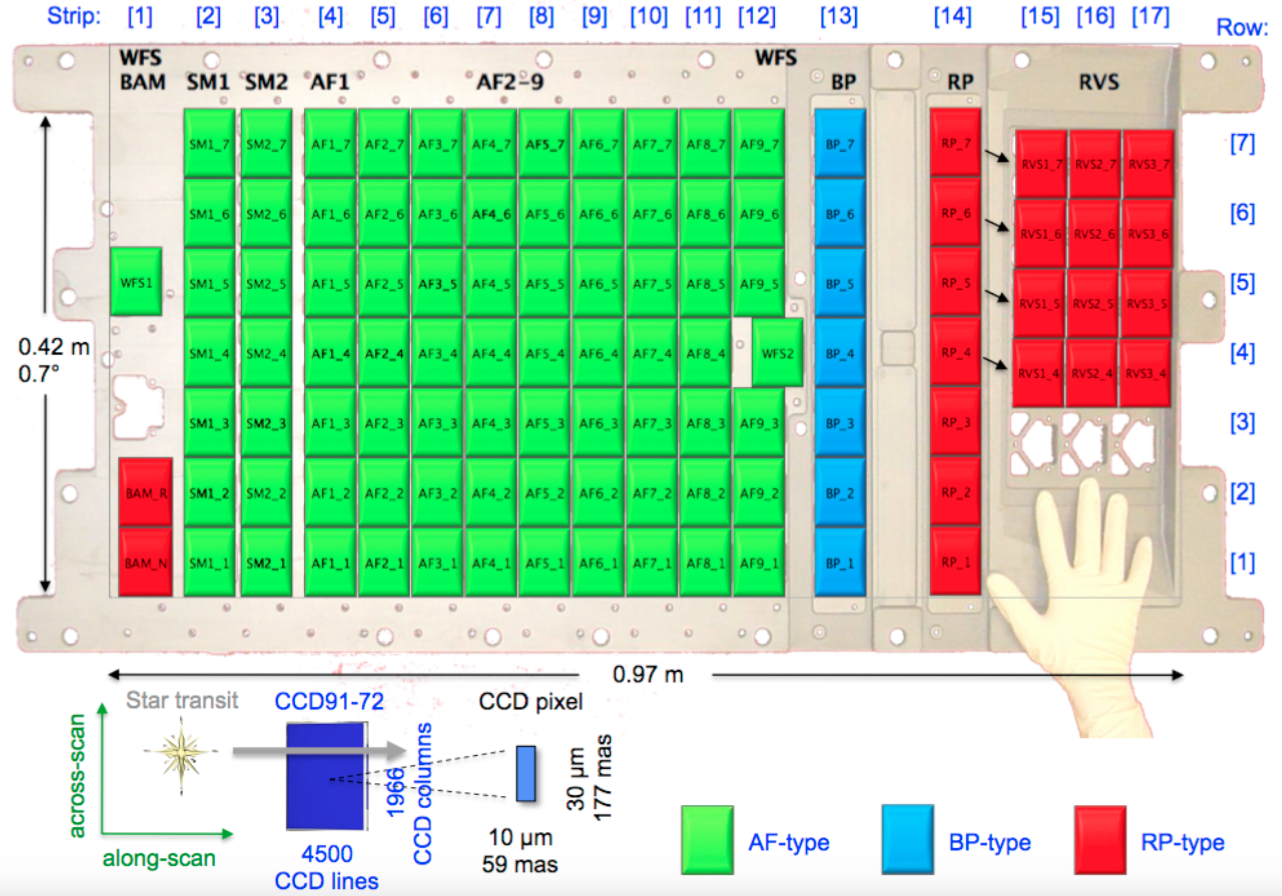
\includegraphics[width=\columnwidth]{gaia_ccd.png}
	\caption{Size comparison and spatial arrangement of the CCD detectors in the Gaia focal plane. Image credit: \citet{2016A&A...595A...1G}.}
	\label{fig:gaia_ccd}
\end{figure}

\section{Gaia}
\label{sec:gaia_data}
Gaia is the one-billion-star surveyor of the European Space Agency (ESA). It has been continuously scanning the sky since July 2014 from its designated location close to the second Lagrange point of the Sun-Earth/Moon system. Gaia’s aim is to map the entire sky,down to magnitude $\sim20.7$, and to collect micro-arcsecond-level astrometry and milli-magnitude-level photometry for the brightest 1,000+ million stars as well as medium-resolution spectroscopy for mainly radial-velocity determination of the brightest subset of $\sim150$ million objects. 

The Gaia scanning of the sky is composed of two independent, superimposed motions: a rotation around the spacecraft spin axis with a period of 6 hours plus a slow, 63 day period precession of the spin axis around the Solar direction at a fixed Solar-aspect angle of $45^\circ$. Over the nominal five-
year mission, Gaia has completed $29$ of these precession periods, leading to an optimally uniform sky coverage with, on average, $\sim70$ astrometric and photometric transits across the focal plane (and $\sim40$ for the spectroscopic instrument). In the extended mission phase that started in July 2019, a similar scanning law is being employed but with a reversed precession direction during the first year. A passage of a star through the focal plane is called a field-of-view transit. During each transit, Gaia collects instantaneous, so-called epoch data of each object. Publication of all epoch data is scheduled (see Table \ref{tab:gaia_drs} for the final data release.

\begin{table}
	\centering
	\caption{Past and future predicted release dates of Gaia data and products.}
	\begin{tabular}{c c}
		\hline
		Release designation & Date \\ 
		\hline
		Gaia DR1 & 14 September 2016 \\
		Gaia DR2 & 25 April 2018 \\
		Gaia EDR3 & 3$^{rd}$ quarter of 2020 \\
		Gaia DR3 & 2$^{nd}$ half of 2021 \\
		Final release & not yet determined \\
		\hline
	\end{tabular}
	\label{tab:gaia_drs}
\end{table}

As the spacecraft slowly rotates, observed stars traverse the Gaia focal plane equipped with 106 CCD detectors (show in Figure \ref{fig:gaia_ccd}). Every star that gets observed therefore passes trough a sequence of those detectors who analyse a star in the given order:

\subsection{Photometry and astrometry}
The first array of CCDs that collects light from stars is a Sky Mapper (SM) that autonomously detect objects. Stars brighter than magnitude $\sim3$ are too bright to be detected automatically. The faint detection threshold is set at $20.7$ magnitude in the Gaia G band but is not infinitely sharp due
to on-the-fly magnitude estimation errors of the on-board software.

After the source detection, stars pass into the largest array of CCDs that is attributed to the Astrometric Field (AF). It collects the instantaneous positions and fluxes of all objects detected by the Sky Mapper as they traverse along the field. Astrometric measurements are made in a white-light bandpass, covering the range from 3300 to 10500 \AA, which is referred to as the Gaia G band.

The last spectro-photometric measurements are thereafter performed by two low dispersion detectors that are measuring precise fluxes in a number of narrow-pass sub-bands of previously mentioned wide-pass G band. The Blue Photometer (BP) collects low resolution spectra of all objects over the wavelength range from 3300 to 6800 \AA. The integrated magnitude is referred to as the G$_{BP}$ or BP magnitude. The Red Photometer (RP) collects low-resolution spectra of all objects over the wavelength range from 6300 to 10500 \AA. The integrated magnitude is referred to as the G$_{RP}$ or RP magnitude.

\subsection{Spectroscopy}
A final measurement performed by the spacecraft is spectroscopy over the whole observed field of the sky. The integral-field Radial Velocity Spectrometer (RVS) \citep{2018A&A...616A...5C} collects medium-resolution spectra (spectral resolving power (R) $\sim11,700$) over the wavelength range from 8450 to 8720 \AA, for all objects brighter than magnitude $\sim16$ in this bandpass. The location of the pass-band is selected to cover the ionised calcium (CaII) triplet with a prominent absorption features over a large temperature range of stars and can therefore be used to determine radial velocity of spectrally diverse stars. The integrated magnitude in the RVS bandpass is referred to as the G$_{RVS}$ magnitude. The RVS has a reduced field of view orthogonal to the scan direction such that fewer observations up to the RVS limiting magnitude are collected compared to photometric fields in a ratio of 4:7.

\section{Gaia DR2}
\label{sec:gaia_dr2_data}
The second data release of Gaia data (Gaia DR2) was heavily used during the production of this thesis, therefore it requires detailed description of provided tables, its use and potential problems. The release set is far from complete and similar to the final release, but on the other hand provides an unprecedented set of homogeneously acquired and reduced stellar informations newer seen before. Visual and numerical representation of the specific stellar product is given in Figure \ref{fig:gaia_drs}. Gaia DR2 is based on data collected by the spacecraft between 25 July 2014 and 23 May 2016, spanning a period of 22 months. 

\begin{figure}
	\centering
	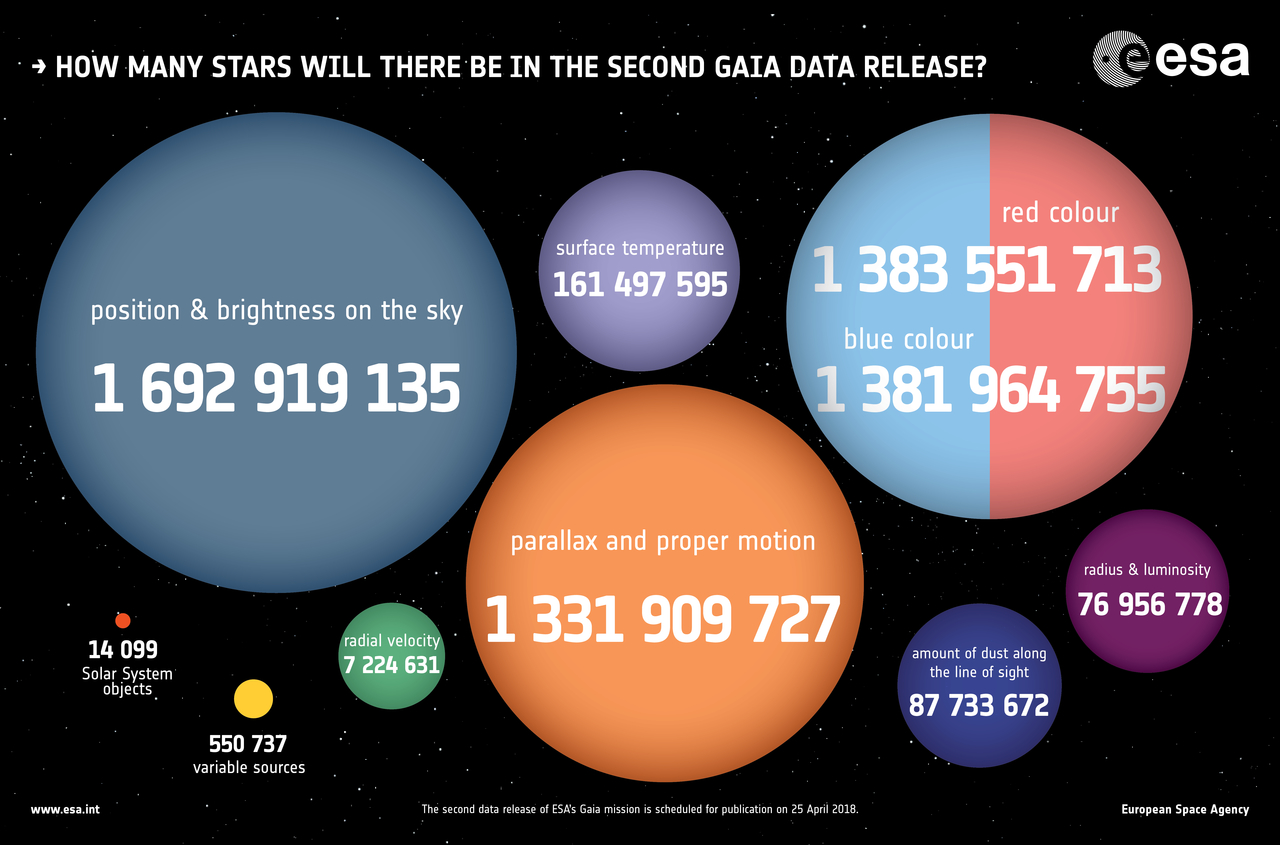
\includegraphics[width=\columnwidth]{1567214817936-Gaia_DR2_numbers_1280.jpg}
	\caption{Visual and numerical representation of Gaia DR2 stellar content. Image credit: ESA, CC BY-SA 3.0 IGO.}
	\label{fig:gaia_drs}
\end{figure}

Along the calibrated raw measurements, Gaia Data Processing and Analysis Consortium (DPAC) provides numerous parameters and properties of stars, pre-selected Solar system bodies and quasars that can be used and explored by users. Among them we can find:
\begin{itemize}
	\item \textbf{Astrometric set} consisting of partial 2-parameter (limited to celestial positions $\alpha$ and $\delta$) and full 5-parameter astrometric solution with addition of including parallax, and proper motion. The 2-parameter sources are typically faint (with about half of them at magnitude G > 20.6), have very few observations (less than five as required for full solution), or very poorly fit the five-parameter astrometric model. All sources fainter than magnitude G = 21 have only positional information. In the current data release all stars are still treated as single during astrometric fit, which could significantly influence solutions in the case of multiple fast moving sources contributing to the position of an observed photocentre. The Gaia coordinate reference frame is aligned with the International Celestial Reference Frame (ICRF) using positions of extragalactic sources such as quasars \citep{2018A&A...616A..14G}. After the initial release, it was determined that the quality of an astrometric fit is best described by the renormalised astrometric chi-square (RUWE) \citep{ruwe}. Further details about astrometric processing and validation are given in \citet{2018A&A...616A...2L, 2018A&A...616A...9L}.
	
	\item \textbf{Photometric data set} contains the broad band photometry in the G, G$_{BP}$, and G$_{RP}$ bands, giving us colour information for Gaia DR2 sources that were observed at least twice. The mean value of the G-band fluxes is reported for all sources while colour information (BP and RP) is available for about 80$\%$ of them.	The integrated colour information suffers from strong systematic effects at the faint end of the survey (G~>~$19$), in crowded regions, and near bright stars. In the case when measured fluxes are inconsistent between the G and the G$_{BP}$ and G$_{RP}$ bands (sum of the later two is significantly larger that G measurement) a warning is raised. A quantitative index of this effect is provided in the numerical form as \textit{flux excess factor}. Further details about processing and photometry validation are given in \citet{2018A&A...616A...4E, 2018A&A...616A...3R}.
	
	\item \textbf{Radial velocity measurements} indicate stellar median radial velocity, averaged over the first 22 months of the observations. Therefore stellar multiplicity and their orbital motion can not be determined from current data. Velocities are provided for sources which are brighter than magnitude 12 in the G$_{RVS}$ photometric band. Because of used set of spectral templates during radial velocity determination, velocities are reported only for stars with effective temperatures in the range between $3550$ and $6900$~K (referring to the effective temperature of a used template and not an actual effective temperature of a star). By the RVS pipeline design, determined absolute radial velocity are limited to $1000$~\kms. The uncertainties of the radial velocities at the faint end depend on stellar effective temperature and range from $1.4$~\kms\ for cooler to $3.6$~\kms\ for hotter stars. The zero-point of the RVS velocities was determined using a comprehensive set of standard stars with numerous dedicated, precise and temporally spread radial velocity measurements \citep{2018A&A...616A...7S}. Further processing details of RVS data are given in \citet{2018A&A...616A...6S}.
	
	\item \textbf{Stellar variability data set} consists of sources that were firmly identified as variable (based on at least two observations of the two Gaia telescopes). The final number still represents only a small subset of the total amount of variables expected in the Gaia survey. The sources were classified into the following nine categories based on their light curves: RR Lyrae (anomalous RRd, RRd, RRab, RRc), long period variables (Mira type and Semi-Regulars), Cepheids (anomalous Cepheids, classical Cepheids, type-II Cepheids), $\delta$ Scuti and SX Phoenicis stars. If a star had 12 or more observations its light curve was analysed in detail. They are designated as specific object studies (SOS) and consist of variables of the type Cepheid
	and RR Lyrae, long period variables, short time scale variables, and rotational modulation variables. Full details on the variable star processing, results and their validation are given in \citet{2018A&A...618A..30H, 2018A&A...618A..58M, 2018A&A...620A.127M, 2019A&A...622A..60C}.
	
	\item \textbf{Astrophysical parameters} derived by the astrophysical parameter inference system in the Gaia data processing (Apsis) include estimates of \Teff\, extinction A$_G$ and reddening E(G$_{BP}$~-~G$_{RP}$), radius, and luminosity for stars brighter than magnitude G~=~17. Values of \Teff\ are reported only over the temperature range between $3000$ and $10,000$~K that is induced by the training set for the algorithm responsible for the \Teff\ estimation. Estimates of the other astrophysical parameters are published for about half of the sources with determined \Teff. As the processing pipeline was performed individually for every object and with a limited set of input data (three Gaia photometric bands and parallax) some errors are expected because of high degeneracy between determined parameters. If a star is located far from expected isochrones used in the processing, extinction becomes overestimated. Full details of the astrophysical parameter processing and result validation are described in \citet{2018A&A...616A...8A}.	
	
	\item \textbf{Solar system objects} (SSO) data set provides epoch astrometry and unfiltered G photometry for a pre-selected list of $14,099$ known minor bodies in the solar system that are numbered in the Minor Planet Center repository. Each time a given SSO enters field of view of Gaia telescopes celestial positions are recorded as seen from the spacecraft. The data set and its production are thoroughly described in \citet{2018A&A...616A..13G}.
	
\end{itemize}

The above sections are partially adapted and summarized from \citet{2016A&A...595A...1G, 2018arXiv180409365G, gaia_primer}.

\section{GALAH}
\label{sec:galah_data}
The GALactic Archaeology with HERMES (GALAH) \citep{2015MNRAS.449.2604D} is an ongoing spectroscopic survey that aims to unveil the Milky Way’s formation history by studying the detailed chemical composition of observed stars. Fossil remnants, which have been disrupted during the formation and are now dispersed around the Galaxy, are tough to have conserved the initial chemical signature of individual galactic components. It is essential to disentangle their formation location and migration history in order to explain current stellar populations. This can be achieved trough the technique of chemical tagging \citep{2002ARA&A..40..487F} that promises identification of old dispersed fossil remnants based on their unique abundance patterns over numerous chemical elements. The GALAH aims to achieve this by measuring up to 31 elemental abundances (from 7 independent element groups with different physical origin) individually in every acquired spectrum.

The GALAH survey was the main driver for the construction of the High Efficiency and Resolution Multi-Element Spectrograph (HERMES) \citep{2010SPIE.7735E..09B, 2015JATIS...1c5002S}, a multi-fibre spectrograph mounted on the $3.9$-metre Anglo-Australian Telescope (AAT) situated at the Siding Spring Observatory, Australia. The spectrograph has a resolving power of R $\sim 28,000$ (or R $\sim 45,000$ when slit mask is used) and covers four separately acquired wavelength ranges (4713 -- 4903~\AA, 5648 -- 5873~\AA, 6478 -- 6737~\AA, and 7585 -- 7887~\AA), together covering approximately 1000~\AA, including the H$\alpha$ and H$\beta$ lines. The ranges are frequently referred to as blue, green, red and near-infrared spectral arms. This configuration can simultaneously record spectra from up to 392 fibres distributed over a $2^\circ$ diameter field of the night sky, with an additional 8 fibres used for the telescope guiding. The spectrograph can typically achieve a signal to noise ratio (SNR) $\sim100$ per resolution element at magnitude V=14 in the red arm during a 1-hour long exposure. 

\subsection{Acquired spectra and target selection}
The spectroscopic data used during the production of this thesis were taken from the pilot survey, the main GALAH survey \citep{2015MNRAS.449.2604D}, the K2-HERMES survey \citep{2018AJ....155...84W}, the TESS-HERMES survey \citep{2018MNRAS.473.2004S}, and special dedicated the HEMRES open clusters (De Silva et al. in preparation) and the HERMES Orion star forming region (Kos et al. in preparation) surveys. Together they form a dataset of $669,845$ successfully reduced stellar spectra, of which a small fraction belongs to a repeated observations. All acquired spectra are homogeneously reduced to one dimensional spectrum, normalised and shifted to stellar reference frame (detailed description in \citet{2017MNRAS.464.1259K}). Combination of those surveys produces increased number of spectra compared to the main GALAH survey, but at the same time breaks rule of a simple unbiased selection function (Sharma et al. in preparation) that is desired for population studies and easier comparison with synthetic galactic models.

The original selection function of the main GALAH survey is separated into two magnitude limited filed selections - bright (10<V<12) and normal (12<V<14) fields whose target selection is colour independent. Used V magnitude is inferred from magnitudes measured by the Two Micron All-Sky Survey (2MASS) \citep{2006AJ....131.1163S} whose photometric bands are shifted into infra-red spectral region. Because of that, some, especially peculiar and variable stars, might have erroneous estimation of V magnitude leading to an underexposure or excessive spectral crosstalk. Because of expected crowding problems (projected diameter of used optical fiber on the sky is equal to $2$\arcsec) observed stars are located at higher Galactic latitudes ($|b|$~>~$10^\circ$) where density of stars is lower. Additional surveys sometimes break those rules by selecting fainter/dimmer stars, going closer to the Galactic plane, employ colour cuts, or favor interesting preselected stars such as K2 \citep{2014PASP..126..398H} targets, TESS \citep{2015JATIS...1a4003R} targets and cluster members. Therefore some care is needed when trying to infer global stellar or galactic properties based on such inhomogeneous selection criteria.

\subsection{Spectral reduction and parameters determination}
Stellar atmospheric parameters and individual elemental abundances derived from normalized spectra, acquired by different surveys, are analysed with the same procedure that slowly evolved and improved during the course of the GALAH survey.

\begin{itemize}
	\item DR1
	\item DR2
	\item DR3
\end{itemize}


adaptation of Spectra Made Easy (SME) \citep{1996A&AS..118..595V, 2017A&A...597A..16P} software that is described in-depth by Buder et al. (in preparation) as part of the latest data release (DR3) of the GALAH spectra and derived parameters.


\section{Asiago}
\label{sec:asiago_data}
Vastly different from the previous two massive all-sky surveys, telescopes at the Asiago site are mainly used for dedicated observations or monitoring of previously selected targets, whose observational and astrophysical potential was identified from all-sky surveys. During our stay at the Asiago observatory, that usually lasted for four consecutive bright nights every month, we used $1.82$~m Copernico telescope located on top of the nearby hill Mount Ekar (Asiago, Italy - altitude of $1,366$~m).

All our observations were performed by the Echelle spectrograph that is mounted on the telescope on days around the full Moon when quality and deepness of photometric observations is heavily reduced. Design of the Echelle instrument and its slit length enables observer to observe only one star a time. Obtained spectra have a resolving power of R$\sim20,000$ and a wide span of wavelengths between $3600$ and $7400$ \AA. They are divided into 30 orders who partially overlap with succeeding and preceding order, providing an undisturbed coverage of observed wavelengths. Acquired spectra are recorded by Andor CCD with the size of $2048 \times 2048$ pixels. This setup enables us to capture spectra of stars with magnitudes V~<~$10$ at high SNR with reasonable exposure time (less than 1 hour per spectrum). Because of the mechanical limitation, observed stars must be positioned at least $15^\circ$ above the local horizon. At those low altitudes, only the brightest stars are reasonable to be observed because of strong atmospheric attenuation.

Combining location of the observatory and above observational limitations with the fact that our interesting stars were selected from the GALAH survey, highly reduces the number of potentially observable objects. To reduce the atmospheric effect effects, we only observed stars which rose at least $30^\circ$ above the local horizon that is equal to having right ascension above $000000^\circ$. As described in more detail below, we used additional Asiago observations to inspect spectroscopic features not accessible by the GALAH spectra and to prolong radial velocity time series of possible multiple stars who could show signs of radial velocity changes not detectable by a single epoch GALAH spectrum.

Additionally to our program observations, we also contributed spectroscopic observations that resulted in published astronomer's telegrams \citep{2019ATel13340....1M} and scientific papers \citep{2019MNRAS.488.5536M}.

\chapter{Chemo-dynamic tracing of open cluster stars}
One of the main goals of the \Gh\ survey is to explore possibilities of chemical tagging for random field and known open cluster stars. A task that sounds easy in theory, but its working applications are far from ready for large spectroscopic surveys. The road to getting precise stellar chemical abundances leads around many different obstacles, which all have an impact on the final determined abundance values whose precision and accuracy dictates the possibility and success of implementing chemical tagging.

In this chapter, we present our exploration of abundances for a few open clusters that were observed as part of multiple different surveys served by the HERMES spectrograph. In Section \ref{sec:intro_tag}, we briefly describe the history of open cluster membership, the evolution of clusters, and means to discover these ongoing processes using stellar abundance information only. Of multiple observed open cluster in the GALAH, we focus only on a small subset of them that have the highest number of members (see Section \ref{sec:galah_clusters} for the complete list). Section \ref{sec:membership_v2} describes the selection of clusters and integration of orbits for stars inside and around the clusters. Chemical signature of field and cluster stars is analysed in Section \ref{sec:chem_ej_tag} and the results are summarised and discussed at the end of this chapter.

\section{Introduction}
\label{sec:intro_tag}
The latest second release of \G\ data (\Gs, \cite{2018A&A...616A...1G}) revolutionized numerous fields of astronomy, including research of galactic open clusters. Its combined information of stellar distance, kinematics, and photometric measurements enables us to go beyond simple methodologies, such as star density counts, to unravel even the faintest and sparsest components of open clusters. So far, many works have been published trying to refine parameters, and membership information of long known open clusters \cite{2017A&A...601A..19G, 2018A&A...618A..93C, 2019A&A...627A..35C} and find new, less numerous or fainter clusters \cite{2019ApJS..245...32L, 2019JKAS...52..145S, 2019A&A...624A.126C, 2020arXiv200107122C}. Such thorough and the improved investigation uncovered that many of the clusters listed in modern catalogues, initially discovered as apparent stellar overdensities, are no more than chance alignments of stars and not true physical clusters \cite{1998A&A...340..402B, 2000A&A...357..145C, 2016AJ....152....7H, 2018MNRAS.480.5242K, 2020A&A...633A..99C}.

Born from the same molecular cloud, open clusters are ideal test structures for different astrophysical principles. Being influenced by external and internal processes, such as tidal stripping and close stellar interactions, their lifetime is limited from about 100 Myr to a few Gyr for the densest structures \cite{1998A&A...337..363P, 2013MNRAS.434.2509M}. This gives us a possibility of observing them at different evolutionary stages \cite{2006BASI...34..153C, 2007A&A...468..139P} before they blend \cite{2001A&A...366..827B} into field stellar population. The most prominent transitional features we can observe are compact cluster tidal tails \cite{2019AA...627A...4R, 2019AJ....157..115Y, 2019AA...621L...3M, 2019arXiv191206657Z} and lose extended halos of evaporated stars. They are observed as a slowly decreasing over-density \cite{2002A&A...385..471C, 2004A&A...427..485B, 2019AA...627A.119C} of stars far from a denser cluster core. Due to close gravitational interactions among members, they can be ejected out of a cluster at high velocities \cite{2009MNRAS.396..570G, 2010MNRAS.402..105G, 2017MNRAS.470.3049R}. Such cluster members can on the sky be found several degrees or even further away from their main cluster body \cite{2007MNRAS.376L..29G, 2018MNRAS.473.4612K, 2019ApJ...884....6M}. Identification of such stars could be done using a chemical tagging procedure, whose importance and potential problems have already been discuses in Section \ref{sec:open_clustesr_tagging}. 

\section{Additional data specifics}
\label{sec:data_clusters}

\subsection{The GALAH and cluster stars}
\label{sec:galah_clusters}
Among the dedicated HERMES cluster observations and other HERMES surveys, such as the main \Gh\ survey, we detected members of known open clusters, whose stellar membership was taken from results published by \citet{2018A&A...618A..93C}. Their clustering methodology relies on the unsupervised membership assignment code called Unsupervised Photometric Membership Assignment in Stellar Clusters (UPMASK, \cite{2014A&A...561A..57K}). Initially, the methodology was designed to find overdensities using only stellar position and photometry. As the methodology is unsupervised and has zero knowledge about physics or input data, \citet{2014A&A...561A..57K} easily applied it to work with astrometric and positional data. Internally UPMASK creates many incarnations of random values from the input data and their uncertainties, selects the four most important principal components, and runs the clustering algorithm on the components. At the end, detected overdensities are compared with random stellar fields and overdensities of the last iteration. Membership probabilities depend on how often a star was inside the relevant overdensity.

As some of the clusters were not targeted intentionally by the surveys or only their cores, the number of observed members and surrounding field stars of interest can vary substantially. The clusters analysed in this paper, having the most significant number of spectroscopic observations are Berkeley 32, NGC 2516, NGC 2112, NGC 6253, Blanco 1, Ruprecht 147, NGC 2632, NGC 2682,  Melotte 22, and Collinder 261. To supplement their selection, we added members of Melotte 25 cluster whose membership selection was performed by us as it was missing in the mentioned published paper \cite{2018A&A...618A..93C}. The first step of our methodology was comparable to UPMASK. Similarly, we generated many incarnations of the data to determine the kinematics of a cluster. It was computed as a median proper motion of the over-density that was closest to the previously known centre at every iteration. After selection in proper motion space, we used the same stars to determine clusters centre in position, distance, and radial velocity. A multivariate Gaussian distribution was fitted at the determined parameter to assess membership probabilities.

\subsection{Gaia}
\label{sec:gaia_clusters}
For a complete 6D positional and kinematics stellar information, we augmented the \Gh\ data with proper motion, parallax and radial velocity from the \Gs\ data-set. As all investigated open cluster stars are located close to the Sun, their distances can be inferred by the inversion of a parallax value ($1 / \varpi$). Of course, we could, at this point, use a bit more accurate distances that were determined using distance priors based on a Galaxy model \cite{2018AJ....156...58B}. The second approach does give more reliable and symmetric distance uncertainties, but does not reduce the elongated shape of stellar clusters (in radial direction away from our location in the Galaxy) as the distance to every star is determined individually. At the same time, more distant stars have grater relative parallax uncertainties which makes it even more difficult to determine distance and shape of a cluster. To get a more realistic shape of a cluster, all member distances would have to analysed at the same time with inclusion of the isochrone information.

The current release of the \G\ data contains magnitude limited range of recovered radial velocities, that are, whenever possible, supplemented or substituted with the \Gh\ measurements of higher accuracy \cite{2018arXiv180406344Z}. Supplemented are mostly stars fainter than currently adopted \G\ RVS \cite{2018A&A...616A...5C} analysis threshold as the GALAH targets are much fainter stars than the RVS limit. The synergy, therefore, increases the set of useful stars in our case.

\section{Cluster and field members}
\label{sec:membership_v2}
The first step in our analysis was the acquisition of data relevant for each cluster identified among the \Gh\ observations. Identification of observed clusters was made by matching observed stars with known cluster members published by \citet{2018A&A...618A..93C}. As some of the clusters had a low number of stars or were proved to be chance alignments of stars \cite{2018MNRAS.480.5242K}, they were not considered in the analysis. Sky coordinates and distances of selected open cluster members (see Section \ref{sec:galah_clusters} for the list of considered clusters) were taken from \citet{2018A&A...618A..93C} and served us as anchors around which we queried the \Gs\ data. A cone query with a radius of $6^\circ$ and distance limit of $\pm900$~pc around a cluster centre was performed to download a subset of the whole dataset. The elongated shape of queried dataset volume is a result of clusters' apparent elongated shape. A bit different volume was used for a nearby and visually extensive cluster Melotte 25, for which we used radius of $12^\circ$ and distance limit of $\pm200$~pc around its centre. 

The downloaded subset included stars with an incomplete set of \G\ parameters. To complement and improve quality of radial velocity measurements, all available \Gh\ velocity estimates in a subset were used to override or supplement \G\ measurements. In the case of multiple \Gh\ observations, a median velocity per star was used. 

The initial open cluster memberships were taken from \citet{2018A&A...618A..93C} but needed some refinement before it was suitable for us. To select as many possible cluster members, the employed membership algorithm did not relay on magnitude limited radial velocity information to assign cluster membership. To make cluster volume more compact and retain only the most probable core members, we discarded all member stars whose radial velocity deviated for more than $5$~\kms\ from the cluster median value of all retrieved members. The used threshold was determined empirically by observing velocity distributions to discard only a few of the most dissimilar stars. The reason behind this velocity limitation will be evident in Section \ref{sec:orbit_tracing} where we try to keep the cluster volume as compact as possible during its integration. This thresholding prevents unwanted pollution of a cluster by field stars during comparison of their chemical signatures in Section \ref{sec:chem_cluster}. 

\subsection{Stellar tracing}
\label{sec:orbit_tracing}
After the selection of open cluster members, we proceeded with the analysis of stellar movements inside and outside the cluster. In order to get the most reliable motion information, only stars with a complete 6D kinematic information (proper motion + radial velocity + sky coordinate + parallax) were considered. No additional \G\ quality flagging was used to remove stars with potentially wrong parameter estimates as we would like to show in the following steps that they could be discovered and eliminated based solely on their chemical composition.

By knowing members of the observed clusters, their current position, and complete motion vectors, we can trace the path of a volume constrained by the cluster stars backwards or forwards in time. This integration procedure was performed by individual integration of cluster stars in axisymmetric gravitational potential (\textit{MWPotential2014} potential described by \citet{2015ApJS..216...29B}) using \GP\ software library version 1.5.0. \cite{2015ApJS..216...29B}. Being interested in the past ejected members of a cluster, we integrated orbits of cluster stars for $120$~Myr (comparable to ages of the youngest open clusters in our set) into their past and saved their location after every step of $20$~kyr. As the integration process relies only on the present uncertain measurements of their velocities and distance, longer integration is not precise or reliable. This uncertainty is observed by the fact that the cluster volume gets larger during backwards integration instead of staying approximately constant as it would in the case of gravitationally bound stellar components. The volume could also keep shrinking during backwards integration if cluster is loosely bound and is already slowly dissipating at the present time. At every integration step, the cluster volume was described by a minimum convex hull defined by its outer-most members. They serve as vertex points of the constructed geometric body. Such a geometrical shape presents the smallest bounding volume with partially flat boundaries which encompasses all considered members.

The next step of our analysis consisted of finding stars in the clusters' immediate neighbourhood that could be traced back to having origin inside the considered open cluster. To filter-out field stars that travel into a completely different direction than the cluster, we discarded all stars whose galactic velocity vector difference towards present cluster velocity vector was >$50$~\kms. This threshold, therefore, defines the fastest possible speed at which stars could have been ejected. Orbits of the remaining set of stars (usually more than half of the queried stars) were integrated using the same configuration as cluster stars described above. At this point, we could investigate which orbit of the field stars crosses clusters' volume at any given integration step.

To get a more descriptive crossing probability, we created $250$ incarnations of every field star. Initial kinematic properties of each incarnation were drawn from the Gaussian distributions of parallax, radial velocity, and proper motion defined by their reported values and uncertainties. After analysing all $250$ orbits of each star, we described its cluster crossing probability by the longest stay inside the cluster volume and  by the percentage of crossing events. For a crossing to be counted as confirmed, a star had to be located inside the cluster volume for at least $0.4$~Myr -- time that is equivalent to $20$ integration steps. The final selection of probable ejected stars consist of stars, whose integration procedure revealed that they were crossing a cluster volume in at least $68$\% of the incarnations and their longest stay there was at least $1$~Myr. Remaining volume crossing stars, that did not meet the criteria, were considered as random field stars. They were also discarded from further analysis as they might, in the case they were real past cluster members, additionally pollute chemical signature of the field population. Summary of investigated and discovered stars for every cluster is given in Table \ref{tab:cluster_stats}.

\begin{table}
	\centering
	\caption{Clusters statistics. Only stars with a complete 6D positional and kinematic information were considered for this statistics and orbit integration analysis. Numbers in columns successively present: number of all stars with complete information, number of analysed stars that meet initial criteria of having the galactic velocity similar to a cluster ($\Delta$v~<~50~\kms), number of stars that do not cross cluster volume during integration, number of possibly ejected stars, and number of cluster members that defined volume of a cluster.}
	\begin{tabular}{l c c c c c }
		\hline
		Cluster & Queried from & Analysed & Field & Possibly & Known \\
		 & \G\ DR2 & stars & stars & ejected & members \\
		\hline \hline
		Berkeley 32  & 11322 & 2659 & 2047 & 125 & 23 \\ 
		Blanco 1     & 5043 & 2734 & 2687 & 15 & 81 \\
		IC 4665      & 15022 & 10155 & 9823 & 26 & 34 \\
		Mamajek 4    & 21776 & 11623 & 10513 & 85 & 48 \\
		Melotte 22   & 9097 & 6335 & 5944 & 105 & 239 \\
		Melotte 25   & 6836 & 3782 & 3511 & 165 & 126 \\
		NGC 1817     & 12826 & 4489 & 4060 & 74 & 54 \\
		NGC 1901     & 12666 & 7323 & 7204 & 19 & 30 \\
		NGC 2112     & 13866 & 6665 & 6323 & 38 & 49 \\
		NGC 2204     & 4314 & 1777 & 1170 & 180 & 59 \\
		NGC 2516     & 17383 & 11906 & 11030 & 315 & 182 \\
		NGC 2548     & 14371 & 9212 & 8842 & 60 & 34 \\
		NGC 2632     & 9951 & 5290 & 4991 & 170 & 222 \\
		NGC 2682     & 10947 & 5244 & 4776 & 226 & 287 \\
		NGC 6253     & 62975 & 30114 & 17267 & 1362 & 64 \\
		Ruprecht 147 & 17749 & 5062 & 4850 & 23 & 103 \\
		\hline
	\end{tabular}
	\label{tab:cluster_stats}
\end{table}

\section{Chemical signature of clusters}
\label{sec:chem_cluster}
After defining potential members of different cluster components (field, ejected, and members), we can look into the abundance signatures of an individual component and their overlap. Of all 30 possible \Gh\ chemical abundances, we initially excluded only Li because of its intrinsic variability that depends on the stellar evolutionary stage. Scatters plots of all considered abundances and \Feh\ as a function of \Teff\ for clusters most populated by the \Gh\ data are shown in Figures \ref{fig:ct_cluster1}, \ref{fig:ct_cluster2}, \ref{fig:ct_cluster3}, and \ref{fig:ct_cluster4}. Not all plots for the same cluster have the equal number of points as reporting of abundance values depends on the estimation of their reliable detectability that is based on equivalent widths of elemental absorption lines (thoroughly described in \citet{buder2020}). The plots show only stars with unflagged (\texttt{flag\_sp} = 0, other flag values are described in \citet{buder2020}) stellar parameters, that are presumably of the highest quality.

\begin{figure}
	\centering
	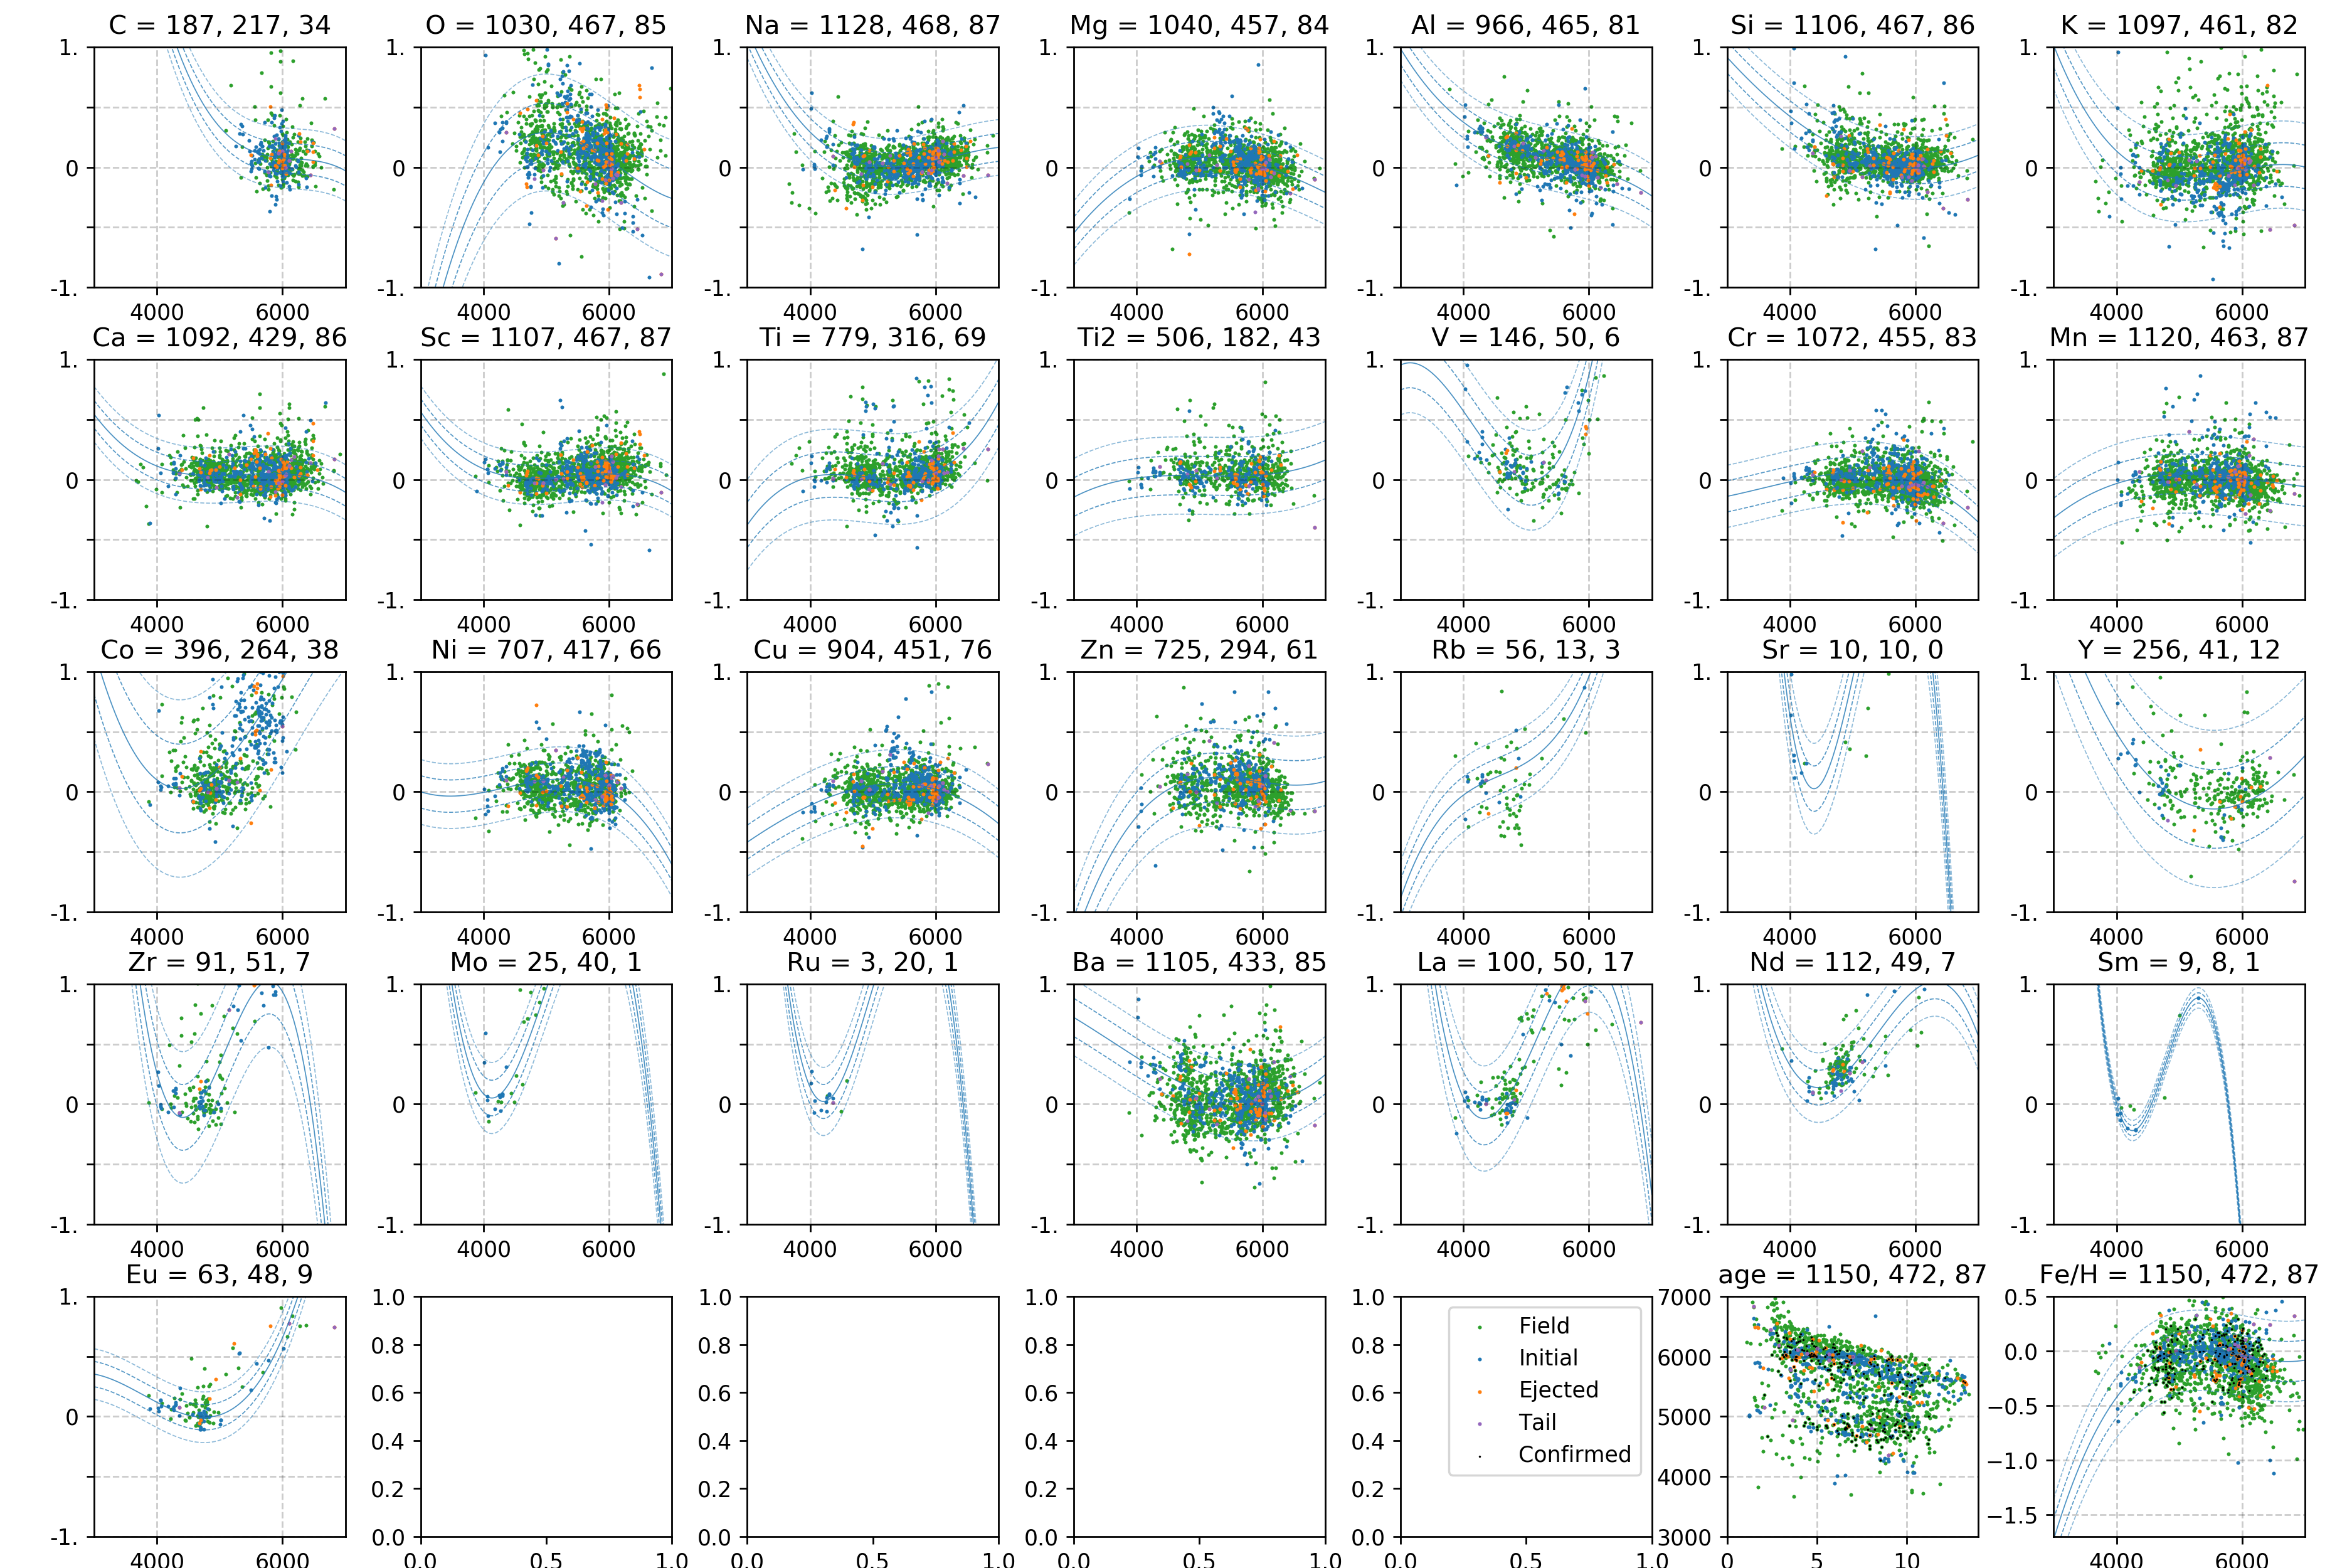
\includegraphics[width=\textwidth]{p_teff_abundances_NGC_2682_orbits_DR3_new_flag0.png}
	\caption{NGC 2632 abundance scatter plots as a function of effective stellar temperature. The solid blue line represents the best fit on the cluster population. The 1$\sigma$ and 2$\sigma$ abundance deviations from the fit are given by dashed blue lines of decreasing intensity. Coloured dots represent field (green), members (blue), and possibly ejected (orange) stars. Their numbers are given above every panel, following the elements' name. Purple dots preset known tails (described later in Section \ref{sec:tails_chem}) of slowly evaporating stars in some clusters. The last two panels present \Teff\ of stars at different ages (in Gyr), and dependence of \Feh\ on their \Teff. The black dots in those two panels indicate possibly ejected stars whose chemistry was matched to cluster stars.}
	\label{fig:ct_cluster1}
\end{figure}

\begin{figure}
	\centering
	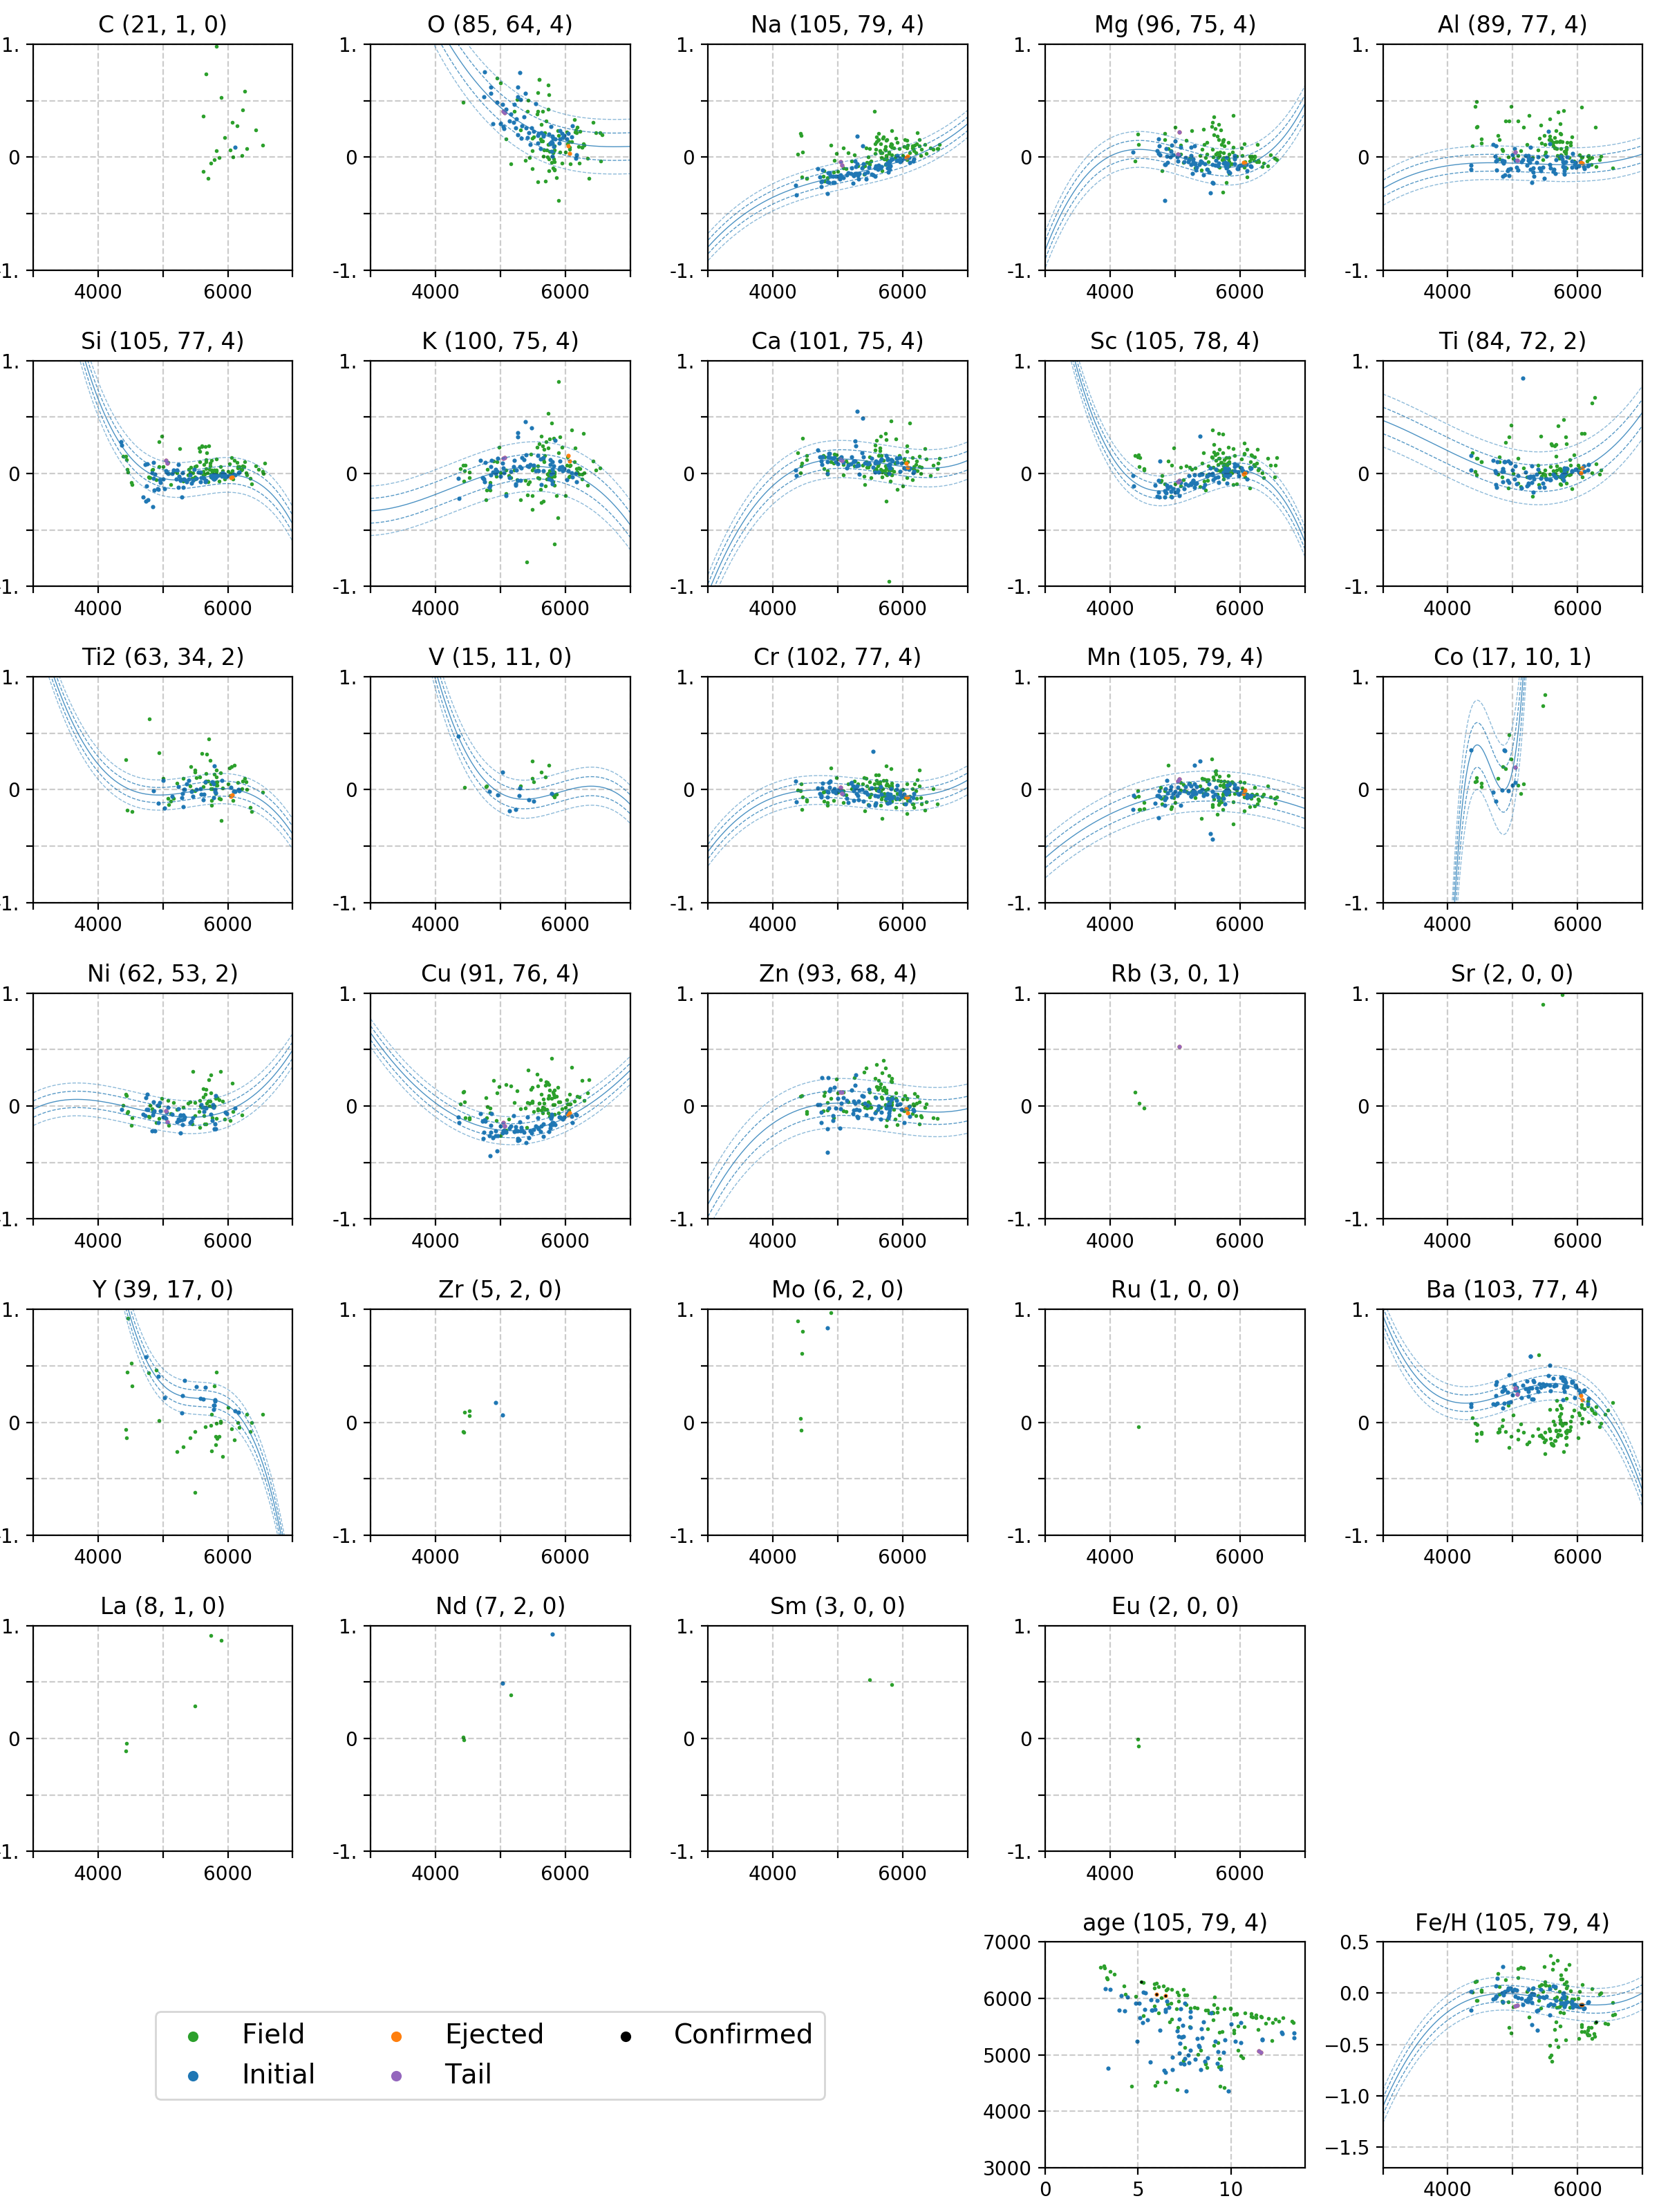
\includegraphics[width=\textwidth]{p_teff_abundances_Blanco_1_orbits_DR3_new_flag0.png}
	\caption{Same plots as in Figure \ref{fig:ct_cluster1} but for open cluster Blanco 1.}
	\label{fig:ct_cluster2}
\end{figure}

\begin{figure}
	\centering
	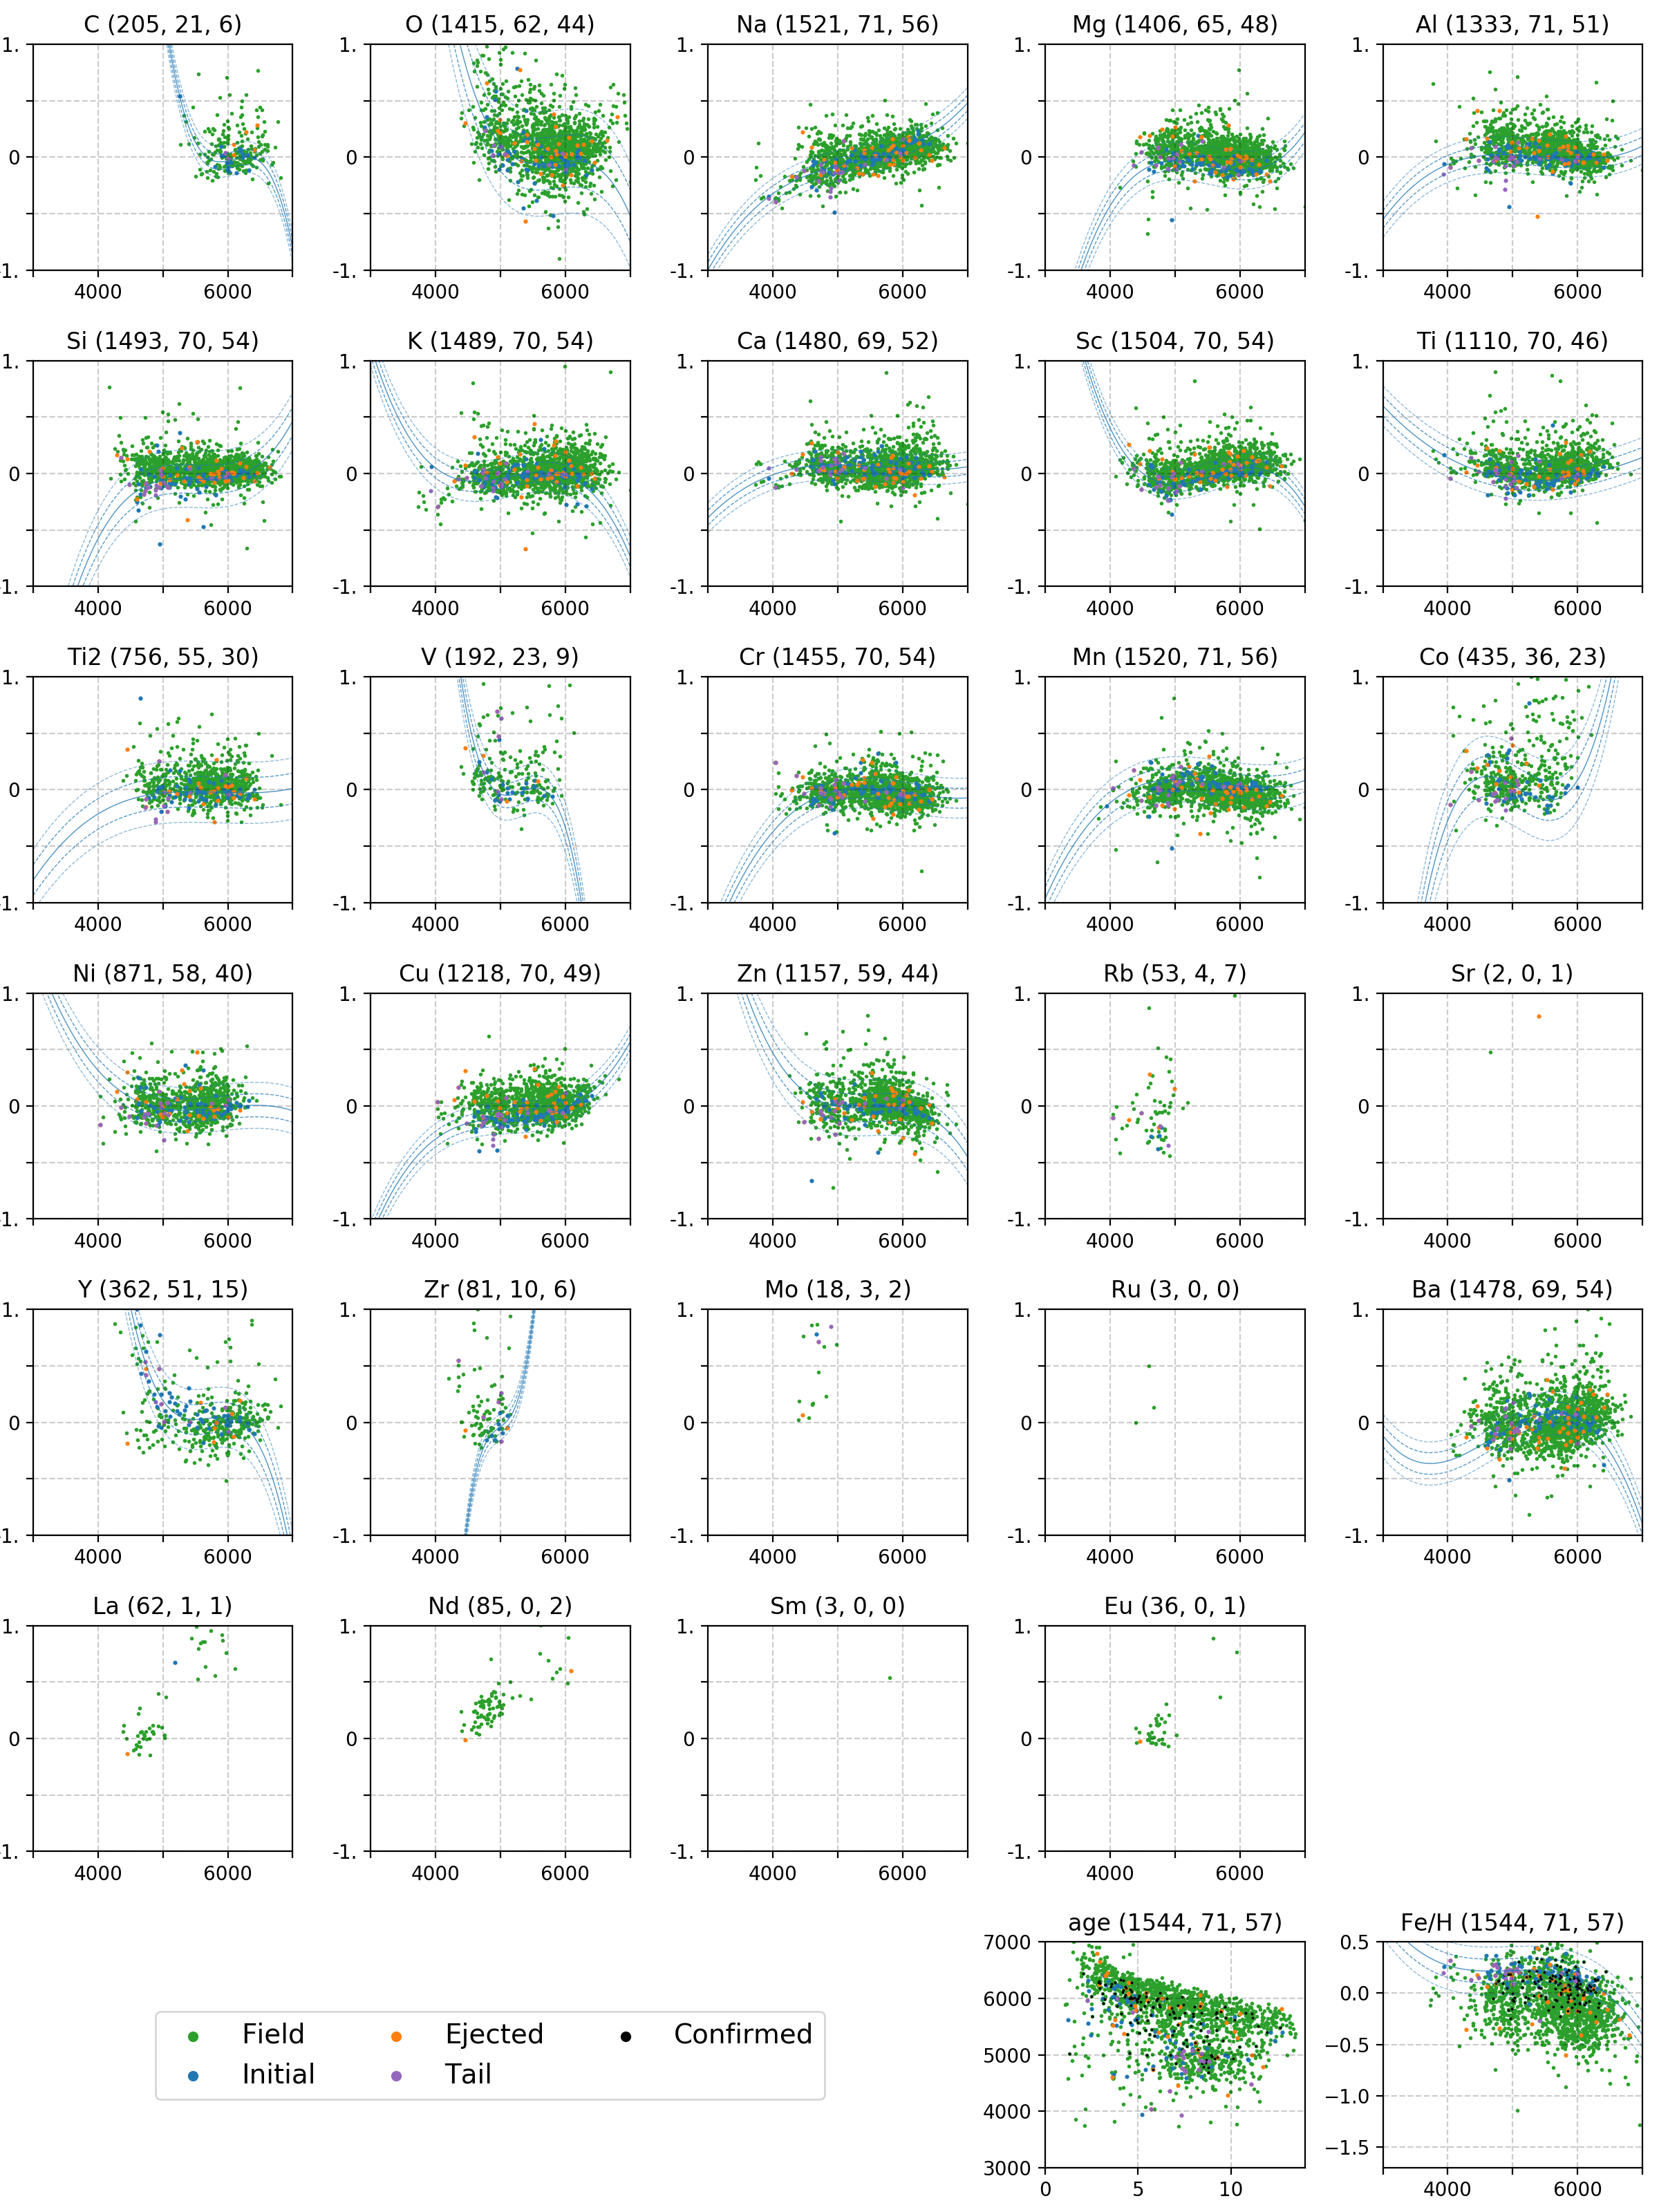
\includegraphics[width=\textwidth]{p_teff_abundances_NGC_2632_orbits_DR3_new_flag0.png}
	\caption{Same plots as in Figure \ref{fig:ct_cluster1} but for open cluster NGC 2632.}
	\label{fig:ct_cluster3}
\end{figure}

\begin{figure}
	\centering
	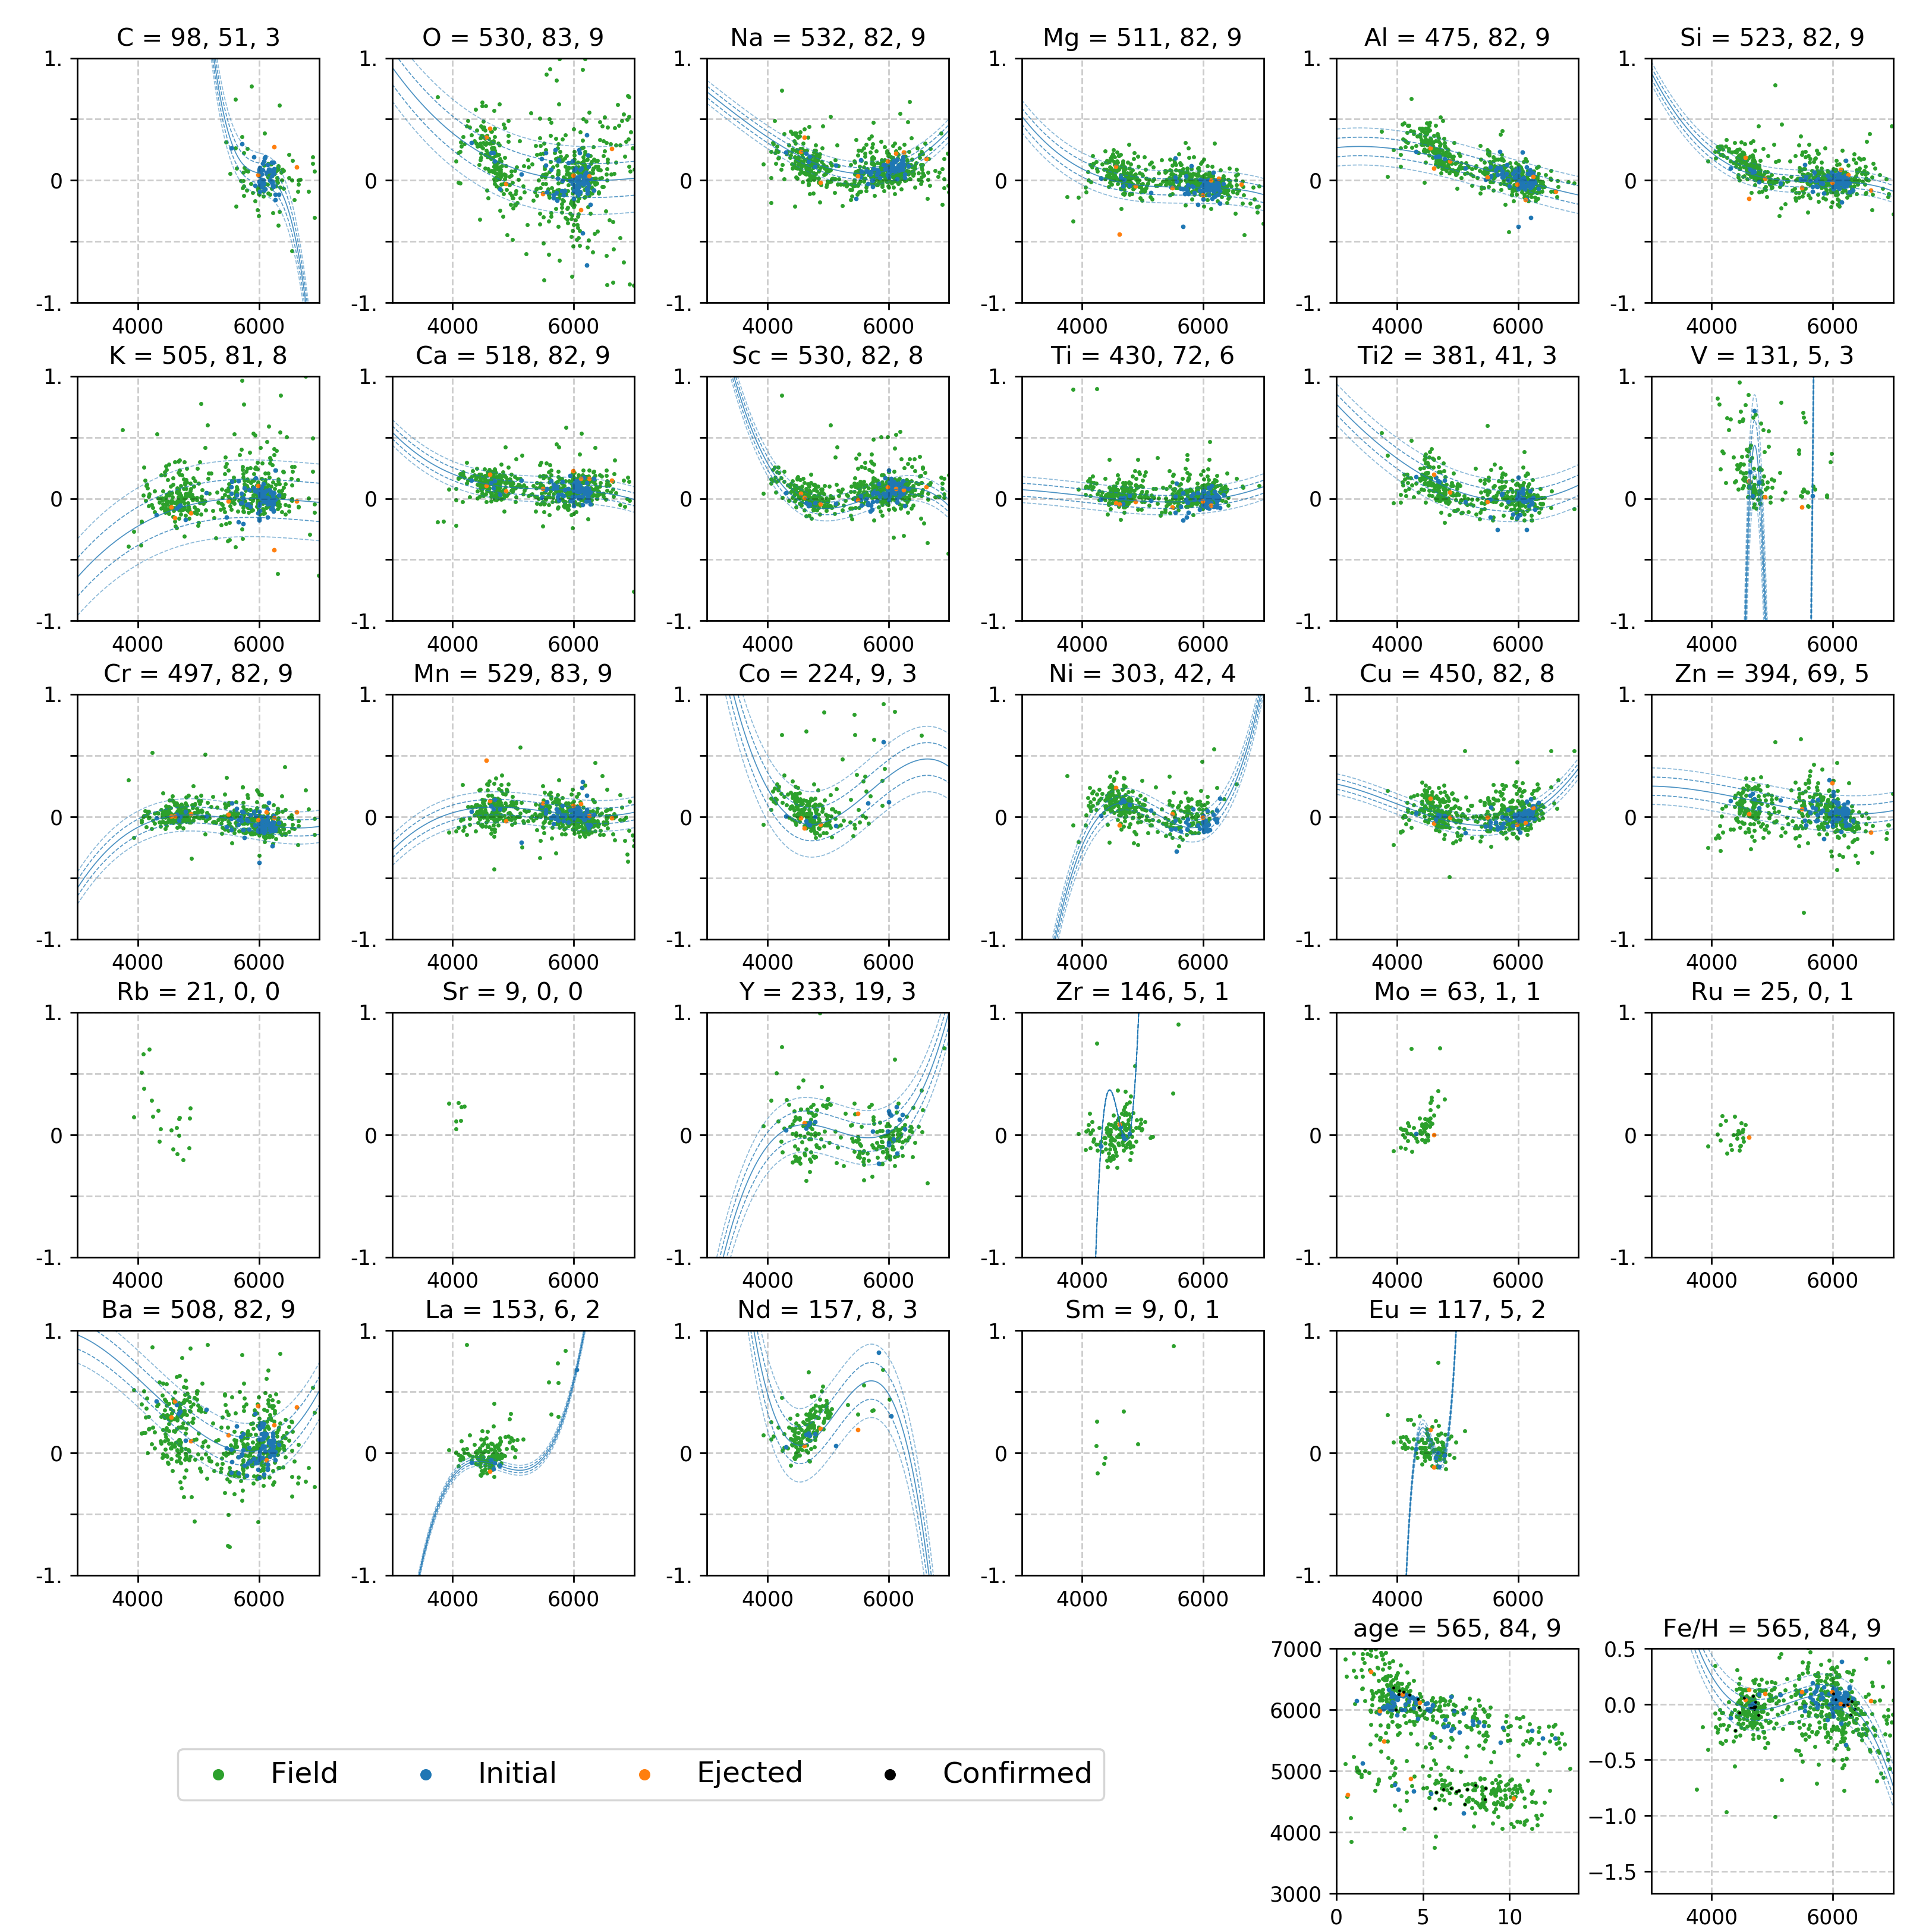
\includegraphics[width=\textwidth]{p_teff_abundances_Ruprecht_147_orbits_DR3_new_flag0.png}
	\caption{Same plots as in Figure \ref{fig:ct_cluster1} but for open cluster Ruprecht 147.}
	\label{fig:ct_cluster4}
\end{figure}

\begin{table}
	\centering
	\caption{The number of acquired \Gh\ spectra among different cluster components that were considered during the chemical comparison. No parameter or abundance flagging was yet used at this point. Stars represented by these statistics are a subset of stars given in Table \ref{tab:cluster_stats}. Because of a small percentage of repeated observations, few clusters (especially NGC 2682 that was used as the calibration and verification field) can have a higher number of spectra than the number of member stars.}
	\begin{tabular}{l c c c }
		\hline
		Cluster & Field & Ejected & Members \\
		\hline \hline
		Berkeley 32  & 42 & 2 & 36 \\ 
		Blanco 1     & 151 & 10 & 109 \\
		IC 4665      & 1114 & 6 & 26 \\
		Mamajek 4    & 2907 & 26 & 13 \\
		Melotte 22   & 1016 & 21 & 67 \\
		Melotte 25   & 653 & 27 & 64 \\
		NGC 1817     & 569 & 11 & 36 \\
		NGC 1901     & 6963 & 19 & 28 \\
		NGC 2112     & 401 & 4 & 66 \\
		NGC 2204     & 129 & 23 & 58 \\
		NGC 2516     & 4604 & 101 & 48 \\
		NGC 2548     & 767 & 6 & 18 \\
		NGC 2632     & 2266 & 77 & 116 \\
		NGC 2682     & 1710 & 147 & 1000 \\
		NGC 6253     & 825 & 34 & 86 \\
		Ruprecht 147 & 798 & 14 & 175 \\
		\hline
	\end{tabular}
	\label{tab:cluster_stats_abund}
\end{table}

\subsection{Abundance and age trends}
\label{sec:abund_trends}
%Ker vidimo in tudi drugi modeli kar mocne trende zastopanosti v odvisnosti od fizikalnih parametrov zvezd, je treba te nekako spraviti na isto raven. Najlazje diferencialno - naredimo fit na kopico in gledamo koliko ostali odstopajo od tega
One of the first things we noticed on the shown abundance scatter plots is their strong dependence on physical parameters, especially \Teff. As this is not the first or unique observation of those trends \cite{2010A&A...523A..71G, 2013ApJ...775...58B, 2016MNRAS.457.3934L, 2018A&A...619A.176B, 2019arXiv191208539C}, they are most likely products of insufficient/inaccurate stellar models and/or actual abundance patterns, and not induced solemnly by the employed \SME\ spectrum analysis pipeline that was used by \citet{buder2020} to determine stellar abundances.

If we presume that observed trends are artificially induced and considered cluster members should have a homogeneous chemical composition that is independent of stellar type, a differential chemical tagging analysis can be used \cite{2019arXiv191208539C}. Such analysis considers only comparisons among stars with a similar set of stellar parameters. To describe observed trends, we independently fitted a 3$^{rd}$ degree polynomial function using $2.5\sigma$ clipping algorithm in 2 steps to every abundance versus \Teff\ diagram. By subtracting fitted trends, we estimated degree of intracluster scatter for every element. Because of limitations of measuring certain abundances, the fit was not performed if the number of valid abundance measurements was lower or equal to a used polynomial degree $+1$.

In the ideal case, all of the trends for the same element observed in different open clusters would have the same shape and would be distinguished only by their abundance offsets that result from their distinct chemical pattern. Looking at our fitted trends, everything is not so simple and easy as the fitted curves can have significantly different shapes. For example, trends of elements Ba and Cu are in general U-shaped. Therefore the highest or lowest abundance values are present in the middle of the \Teff\ region. Those results imply that using the latest \Gh\ abundances, we can not easily find the global behaviour of measured elements. Blindly using the wrong trend line would, therefore completely change results in our case.

Additional identification that there might something be wrong with the parameters lies in the determined ages of individual stars in the clusters. The ages are determined by the best fitting isochrone with appropriate stellar \Feh\ that lies closest to the stars' position on H-R diagram (further details in \citet{buder2020}). As the procedure is run independently for every star in the survey, ages among cluster stars (see plots in Figures \ref{fig:ct_cluster1}, \ref{fig:ct_cluster2}, \ref{fig:ct_cluster3}, and \ref{fig:ct_cluster4}) are strewn over a range of 5~Gyr or more. Fortunately the abundance computation does not require information about the stellar age, but they both share the requirement for an accurate information about the basic stellar parameters.

% TODO Fino bi bilo (morda tudi na grafu) nekako označiti privzeto starost te kopice. Starost ima gotovo tudi precejšnje napake - najbrž je najbolj točna za MSTO (če jih imaš že kaj), pa morda tudi za hladne, ki se šele usedajo na MS. Komentarji tega tipa sodijo v glavni tekst, tu le omeniš, da so tam.

\subsection{Determining chemical similarity}
\label{sec:chem_ej_tag}
%Pogledamo trende in fite, ter koliko moznih izvzenih zvezd se poraja in sklada s temi kemicnimi trendi. Morda nek threshold koliko je dobrih oziroma skladnih s samo kopico, saj ima tudi ta le kar nekaj razpona v izmerjenih/izracunanih vrednostih parametrov.
Having an analytical description of an individual abundance behaviour for every cluster, we can estimate how many and how accurately do the identified ejected stars match with cluster abundance patterns and trends. The most straightforward way to perform this is to count how often does abundance value of an investigated star fall inside a $1\sigma$ (or $2\sigma$ for a more relaxed selection) region around an abundance trend. Both regions and fitted trends are visualised in Figures \ref{fig:ct_cluster1}, \ref{fig:ct_cluster2}, \ref{fig:ct_cluster3}, and \ref{fig:ct_cluster4}. Before performing such counting, we additionally omitted abundance trends of the following chemical elements: V, Rb, Sr, Y, Zr, Mo, Ru, La, and Sm. Their low number of successful measurements per cluster and uncertain trends were not beneficial to the whole chemical tagging experiment and influenced only a small fraction of stars. In general it is not advised to reduce the dimensionality of chemical space for greater differentiation between chemical signatures. As this was one of the first experiments analysing whether the latest \Gh\ DR3 abundances could be used for cluster and global blind tagging, we tried to remove as many additional systematic effects of uncertain measurements as possible. In our case, an individual star was counted as chemically similar if it matched (e.g. fell inside selected $\sigma$ region around the fitted trend line) to a cluster in at least $68$\% of the considered abundances with valid trend fit. Chemically similarity of ejected stars, given as percentage of tagged stars, is presented in Table \ref{tab:cluster_stats_abundtag}.

% TODO To je ok za tabelo 3.3. Morda pa bi v diskusiji tabele 3.3 bilo smiselno pogledati, kako se obnašajo posamezni elementi, recimo ali so še kakšni poleg V, Rb, Sr,... ki zganjajo probleme. Morda tudi, v katere skupine sodijo: a se recimo vsi slow-r elementi obnašajo podobno ali ne. Če se odločiš iti po tej poti, je potem to o različnih kanalih nastajanja elementov dati v uvodna poglavja.

\subsection{Tagging remaining field stars}
\label{sec:chem_fi_tag}
%Kaj se zgodi ce iste kemicne informacije in thresholde uporabimo se za ostale analizirane zvezde v bljizini. Dobimo sploh kaj zvezd ven iz tega in kaksen bi bil v tem primeru njihov kinematicni vektor.
The same principle can also be applied to remaining nearby field stars. As clearly evident from Figures \ref{fig:ct_cluster1}, \ref{fig:ct_cluster2}, \ref{fig:ct_cluster3}, and \ref{fig:ct_cluster4}, the cluster abundances are mostly similar to field stars and lie close to their densest regions in shown abundance scatter plots. Therefore, we were interested in the probability of a random field star being chemically similar to a nearby open cluster. In contrast, some of the investigated clusters, especially Blanco 1, show evident signs of being chemically separable from neighbouring stellar populations. Elements crucial for the populations' separation are commonly used as chemical tracers of galactic evolution and stellar age \cite{2003A&A...410..527B, 2018MNRAS.474.2580S, 2020MNRAS.491.2043L}. Therefore a young cluster, such as Blanco 1, that is located at high galactic latitudes, far from the main galactic plane, can locally be separated from its neighbouring stars. Something that is not common for typical open clusters that can currently be observed in the sky as they mainly reside close to the Galactic plane.

For the field chemical tagging procedure, we used the same selection principle as previously described in Section \ref{sec:chem_ej_tag}. The results of both tagging experiments are together presented in Table \ref{tab:cluster_stats_abundtag}. Even if the abundance distributions of cluster and field stars are intertwined, the results of the tagging experiment are encouraging, as it was more likely that kinematically tracked stars were chemically similar to open cluster than a random nearby field star. The percentage of tagged ejected stars for almost all clusters in Table \ref{tab:cluster_stats_abundtag} is higher than percentage of tagged  field stars. Clusters with zero tagging success suffer the curse of having low number statistics as they have only few possible candidates. For those clusters, if only one ejected star would be tagged, the probability would again be much higher than for the field stars. 

\begin{table}
	\centering
	\caption{Number and percentage of all considered and chemically similar (tagged) stars in the spatial neighbourhood around the analysed open clusters. Percentages indicate the number of stars in different components that are similar to cluster abundance pattern and scatter. Tagging algorithm is detailed in Section \ref{sec:chem_ej_tag}. Only spectra with unflagged stellar parameters were used to produce shown statistics.}
	\begin{tabular}{l c c c c }
		\hline
		Cluster & \multicolumn{2}{c}{Ejected stars}  & \multicolumn{2}{c}{Field stars} \\
		 & All & Tagged & All & Tagged \\
		\hline \hline
		Berkeley 32  & 2 & 0 (0.0\%) & 39 & 2 (5.1\%) \\ 
		Blanco 1     & 4 & 2 (50.0\%) & 150 & 1 (1.0\%) \\
		IC 4665      & 4 & 0 (0.0\%) & 919 & 0 (0.0\%) \\
		Mamajek 4    & 25 & 6 (24.0\%) & 2300 & 82 (3.6\%) \\
		Melotte 22   & 10 & 1 (10.0\%) & 724 & 33 (4.6\%) \\
		Melotte 25   & 15 & 3 (20.0\%) & 389 & 71 (18.3\%) \\
		NGC 1817     & 6 & 0 (0.0\%) & 432 & 4 (0.9\%) \\
		NGC 1901     & 19 & 4 (21.1\%) & 5582 & 5824 (14.8\%) \\
		NGC 2112     & 4 & 0 (0.0\%) & 268 & 7 (2.6\%) \\
		NGC 2204     & 18 & 2 (16.7\%) & 113 & 14 (12.4\%) \\
		NGC 2516     & 71 & 4 (5.6\%) & 3330 & 90 (2.7\%) \\
		NGC 2548     & 5 & 0 (0.0\%) & 605 & 5 (0.8\%) \\
		NGC 2632     & 56 & 13 (22.8\%) & 1544 & 126 (8.2\%) \\
		NGC 2682     & 87 & 33 (37.6\%) & 1150 & 218 (19.0\%) \\
		NGC 6253     & 27 & 3 (11.1\%) & 653 & 21 (3.2\%) \\
		Ruprecht 147 & 9 & 0 (0.0\%) & 565 & 19 (3.4\%) \\
		\hline
	\end{tabular}
	\label{tab:cluster_stats_abundtag}
\end{table}

\section{Comparison with known tidal structures}
\label{sec:tails_chem}
%Izvedli bi krajso primerjavo kako v luci nasih dognanj vidimo plimske repe kopic, ki so jih zaznali drugi.
In the previous section, we analysed stars whose integrated orbits indicate that they could be ejected from neighbouring open cluster sometime in the last 120~Myr. Depending on the mass of involved stars and their proximity during the slingshot mechanism, stars could be thrown out of a cluster into the interstellar space at random velocities and directions. This is true in the case when we presume that stars have no preferential way of moving inside a cluster. Such a process would therefore form a sphere of candidates around the main cluster. The density of candidates would isotropically decrease in all radial directions away from the centre of a cluster, until the effect of the stars being on different orbits in the Galactic potential became important. This effect is also visible in Figure \ref{fig:ejected_around_cluster}, where ejection candidates are scattered all around the confirmed cluster members. A bit denser population of candidates is evident alongside the cluster volume, which probably corresponds to nearby initial cluster members that were discarded due to their mismatching radial velocity as described in Section \ref{sec:membership_v2}.

\begin{figure}
	\centering
	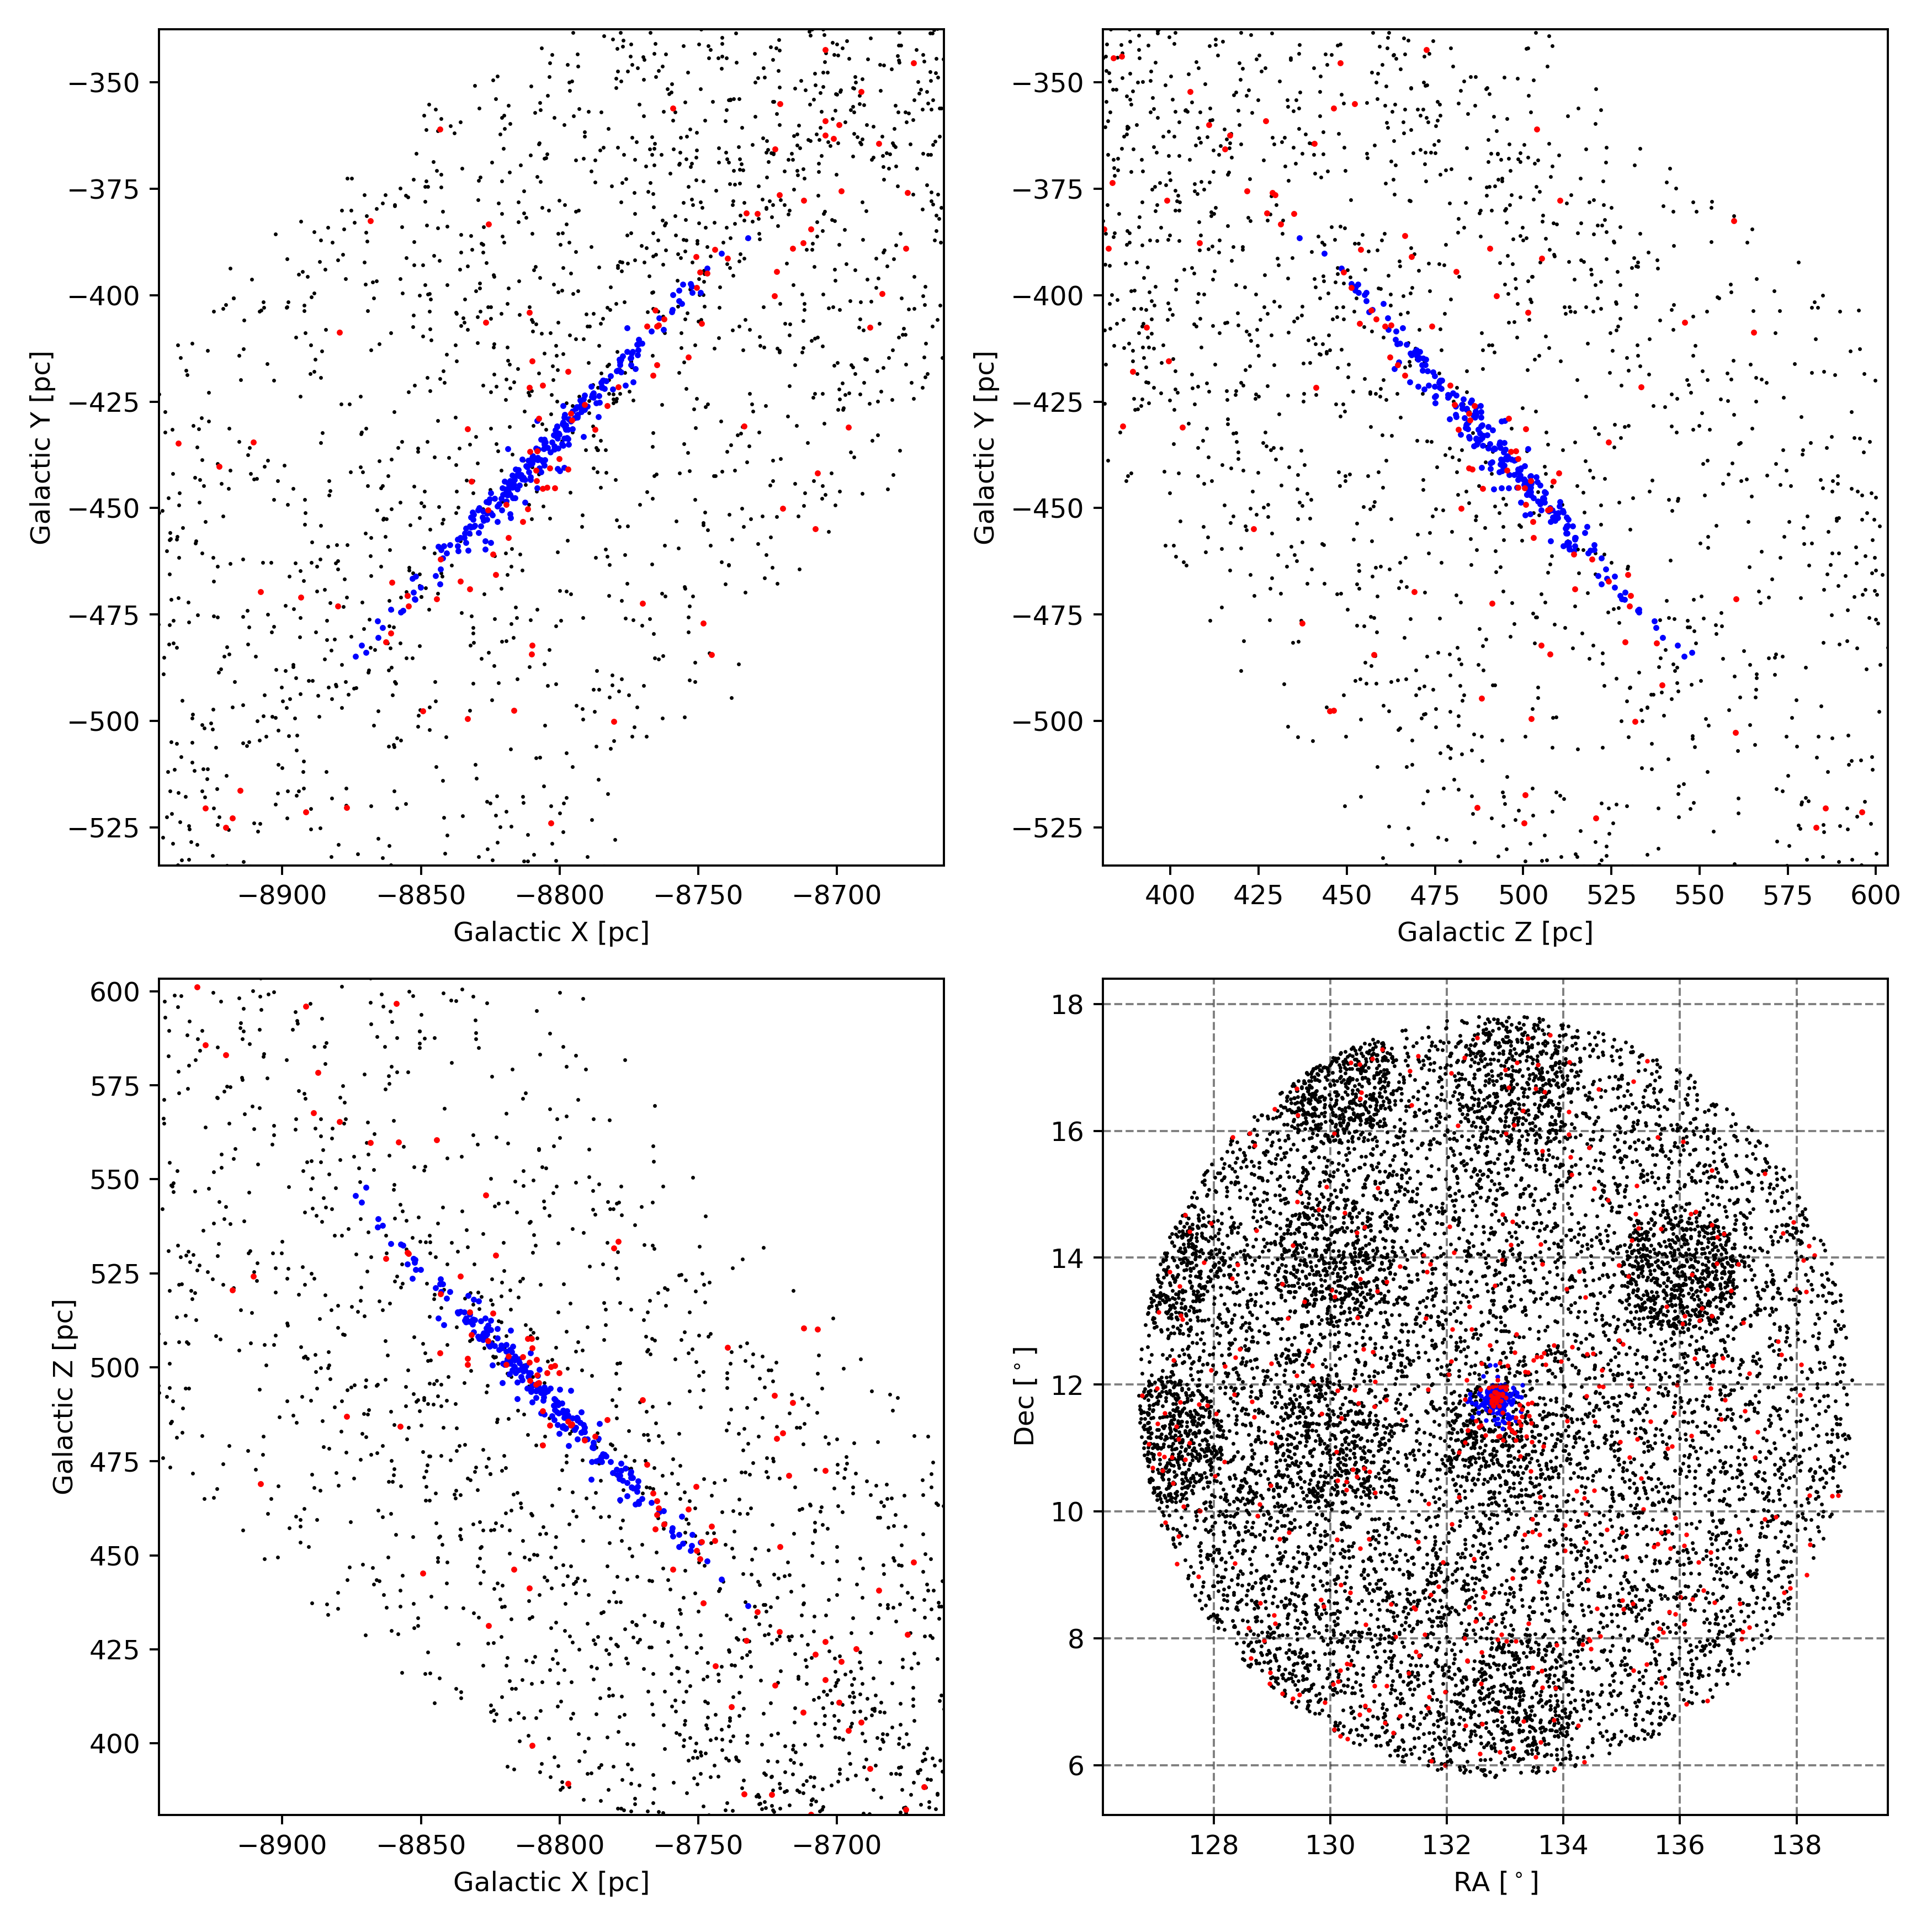
\includegraphics[width=\textwidth]{NGC_2682_possible_ejected-step1.png}
	\caption{Plots show the spatial distribution of the ejected candidates in red around the definite cluster members in blue. All other stars considered in the analysis are shown as black dots. First three panel shows the Galactic position of described cluster components. The denser circular patches of stars in the bottom right panel are not real stellar overdensities, but indicate regions where combined radial velocities of \G\ and \Gh\ are used. The example is given for the open cluster NGC 2682, which has the highest number of potentially ejected stars. Uncertainty of determined stellar distance is clearly evident as elongation of the main cluster body in the radial direction, away from the observers' position.}
	\label{fig:ejected_around_cluster}
\end{figure}

A much less energetic and more gradual mechanism that also influences the lifetime of an open cluster is tidal stripping of stars \cite{2006A&A...455L..17L}. It happens during clusters' journey through a more densely populated region such as galactic spiral arms. Tails reaching out of a cluster would, therefore, have elongated, probably slightly bent shape (not to be confused by the elongated cluster shape in Figure \ref{fig:ejected_around_cluster}), and not a spherical distribution as considered for ejection mechanism. In this section, we compare the chemical composition of known tidal structures (discovered in \Gs\ data by \citet{2019AA...627A...4R, 2019AA...627A.119C, 2019AA...621L...3M, 2019arXiv191206657Z}) of a few the \Gh\ open clusters with other previously defined and analysed structures. All of the aforementioned tidal structures were identified by different clustering methods of the same \G\ data and should, therefore, be in a sense similar to results of our orbital classification procedure. From the published tidal structures \cite{2019AA...627A...4R, 2019AA...627A.119C, 2019AA...621L...3M, 2019arXiv191206657Z}, we first removed all cluster members that were already identified by \citet{2018A&A...618A..93C} and consequently used in our procedure for the definition of clusters' chemical signature. In that way, our possibly ejected stars and tidal structures can be compared directly. Their overlap is shown in the fourth and fifth column of Table \ref{tab:cluster_stats_tails}. As the overlap between them is not zero, we can reliably say that we are all detecting similar kinematic structures using completely different approaches (but the same \G\ data). The identified structures therefore may or might not be related to neighbouring open cluster.

\begin{sidewaystable}
	\centering
	\caption{Statistics of detected stellar tidal structures around some of the clusters that were observed by the \Gh. The columns shown in the following order give information about: name of the analysed cluster, number of all stars found in the surrounding tidal structure, number of stars without cluster members, size of overlap between ejected and tail, number of unflagged \Gh\ observations among tidal structure, chemical similarity with parent open cluster, and reference source of the used data.}
	\begin{tabular}{l c c c c c r }
		\hline
		Cluster & Stars in & Without used & Common with & \Gh\ unflagged & Chemically & Membership\\
		& reference & cluster members & ejected & parameters (\% in & tagged & reference\\
		&  &  & (\% of ejected) & common with ejected) & (\% of valid) & \\
		\hline \hline
		Blanco 1   & 644 & 276 & 3 (50\%) & 7 (42.9\%) & 0 (0.0\%) & \citet{2019arXiv191206657Z} \\
		NGC 2632   & 1393 & 738 & 17 (22.1\%) & 25 (68\%) & 7 (28.0\%) & \citet{2019AA...627A...4R} \\
		NGC 2682   & 952 & 241 & 13 (14.4\%) & 18 (72.2\%) & 6 (33.3\%) & \citet{2019AA...627A.119C} \\
		Melotte 25 & 238 & 238 & 8 (30.8\%) & 57 (14.0\%) & 1 (1.8\%) & \citet{2019AA...621L...3M} \\
		\hline
	\end{tabular}
	\label{tab:cluster_stats_tails}
\end{sidewaystable}

Among randomly acquired The \Gh\ spectra, we observed some stars that where identified to belong to the kinematically discovered tidal structures around open clusters. If we consider only stars with unflagged the \Gh\ stellar parameters, the overlap between the sets is quite significant as more than 50\% of unflagged tail stars were also identified as possible ejected for every studied cluster. This significant overlap reduces probability of the tails having a completely different chemical signature than our selections, but at the same time confirms validity of our orbit tracing approach. 

For a tidal tail chemical tagging procedure, we used the same selection principle as previously described in Section \ref{sec:chem_ej_tag}. The results of the tagging experiment are presented in the last column of Table \ref{tab:cluster_stats_tails}. Majority of the tails have quite significant probability of being chemically similar to a nearby open cluster. 

\section{Summary and conclusions}
\label{sec:clusters_summary_conclusions}
Open clusters, as long known and widely studied stellar structures, still provide many opportunities for their exploration using new and improved information about their stellar components and neighbouring environment. In this chapter, we explored the latest multidimensional abundance data determined for stars observed in the scope of the \Gh\ survey, whose targets also consisted of stars in multiple open clusters. Combined with the \G\ kinematic information, a precise position, shape, and velocity of the cluster volume can be defined. We used the method of backward orbit integration to determine if any of the neighbouring stars could be kinematically traced back to the cluster and have the same chemical signature.

To verify that our orbital integration methodology gives sensible results, they were compared towards identified cluster tidal structures around the same open clusters. Given non zero overlap in all cases, we are confident that our structures are also related to the main cluster body.

Deepened analysis of field and cluster abundance patterns showed improvement in the quality of determined abundances (in comparison towards older \Gh\ releases), but at the same time revealed the pitfalls of blindly using massively determined abundances for blind chemical tagging experiments that are highly desired in the community of galactic archaeology. Identified problems can successfully be overcome by applying differential analysis, which in our case showed some encouraging success of using the \Gh\ abundance data as tracers of stellar birth signatures of individual stars. The tagging experiment showed that it was more likely that we could chemically tag a kinematically pre-selected star than a random nearby star. For a much firmer confirmation, we would require more observations as some of the cluster components were sparsely observed by the \Gh.

The explored methodology depends on the quality and correctness of the determined abundance trends. From the current data, it seems that identified abundance trends are valid only for an individual cluster as they can vary among them. This decreases possibility of preforming differential chemical tagging on larger, potentially galactic, scales.

To improve the parameters used in this chapter, we would have to analyse cluster members as a homogeneous structure that was formed at the same time. This adoption of formation time would force the use of a single isochrone and stellar age for all members, improving their determined \Logg, \Feh, and consequently also stellar surface chemical composition. Our first experiments with the mentioned analysis upgrade already show significant improvements in the stability of the trends and reduction of abundance scatter among cluster members.

\chapter{Peculiar stars}

\section{Abstract}
	Swan bands  -- characteristic molecular absorption features of the C$_2$ molecule -- are a spectroscopic signature of carbon-enhanced stars. They can also be used to identify carbon-enhanced metal-poor (CEMP) stars. The GALAH (GALactic Archaeology with Hermes) is a magnitude-limited survey of stars producing high-resolution, high signal-to-noise spectra. We used 627,708 GALAH spectra to search for carbon-enhanced stars with a supervised and unsupervised classification algorithm, relying on the imprint of the Swan bands. We identified 918 carbon-enhanced stars, including 12 already described in the literature. An unbiased selection function of the GALAH survey allows us to perform a population study of carbon-enhanced stars. Most of them are giants, out of which we find 28 CEMP candidates. A large fraction of our carbon-enhanced stars with repeated observations show variation in radial velocity, hinting that there is a large fraction of variables among them. 32 of the detected stars also show strong Lithium enhancement in their spectra.

\section{Introduction}
Chemically peculiar stars whose spectra are dominated by carbon molecular bands were first identified by \citet{1869AN.....73..129S}. Their spectra are characterised by enhanced carbon absorption bands of CH, CN, SiC$_2$, and C$_{2}$ molecules, also known as Swan bands. Possible sources of enhancement are dredge-up events in evolved stars \citep{1983ApJ...275L..65I}, enrichment by carbon-rich stellar winds from a pulsating asymptotic giant branch (AGB) star, which settles on a main sequence companion \citep{1995MNRAS.277.1443H}, or it can be the result of a primordial enrichment \citep{2016ApJ...833...20Y}. Historically, high latitude carbon stars, presumed to be giants, were used as probes to measure the Galactic rotation curve \citep{2013Ap.....56...68B}, velocity dispersion in the Galactic halo \citep{1991AJ....101.2220B}, and to trace the gravitational potential of the Galaxy.  

Because of their strong spectral features, the most prominent candidates can easily be identified from large photometric surveys \citep{2002AJ....124.1651M, 2004AJ....127.2838D}. Specific photometric systems \citep{1960MNRAS.120..287G, 1968AJ.....73..313M, 1970A&AS....1..199H} were defined in the past to discover and further classify stars with enhanced carbon features in their spectra. Specifics of those systems were catalogued, compared, and homogenised by \citet{2000A&AS..147..361M} and \citet{2003A&A...401..781F}.

Other useful data come from low-resolution spectroscopic surveys, whose classification identified from a few hundred to a few thousand of those objects \citep{2001A&A...375..366C, 2013ApJ...765...12G, 2013AJ....146..132L, 2016ApJS..226....1J, 2018ApJS..234...31L}. High-resolution spectroscopy is required to search for candidates with less pronounced molecular absorption features or to determine their stellar chemical composition. Multiple studies have been carried out to determine accurate abundances of metal-poor stars \citep{1997ApJ...488..350N, 2002ApJ...567.1166A, 2004A&A...416.1117C, 2005ESASP.560..433B, 2006AJ....132..137C, 2007ApJ...655..492A, 2007ApJ...670..774N, 2011ApJ...742...54H, 2013ApJ...762...26Y, 2014AJ....147..136R, 2015ApJ...807..173H, 2015ApJ...807..171J}. Such detailed abundance information is especially important for the analysis and classification of chemically peculiar objects \citep{2013ApJ...778...56C}.

Today, the most sought after, of all carbon-enhanced stars, are the carbon-enhanced metal-poor (CEMP) ones whose fraction, among metal-poor stars, increases with decreasing metallicity \Meh\ \citep{1992AJ....103.1987B, 1997ApJ...488..350N, 1999ASPC..165..264R, 2005ApJ...633L.109C, 2005ApJ...625..825L, 2005AJ....130.2804R, 2006ApJ...652.1585F, 2007PhDT........22M, 2012ApJ...744..195C, 2013AJ....146..132L, 2013ApJ...762...27Y,  2014ApJ...797...21P, 2018ApJ...861..146Y}. Amongst these, those near the main-sequence turn-off are expected to be of particular importance, as they may have accreted enough material from their AGB companion to produce an observable change in their atmospheric chemical composition \citep{2004ApJ...611..476S, 2014MNRAS.441.1217S, 2015ApJ...807..173H}. The accreted material could provide insight into the production efficiency of neutron capture elements in AGB stars \citep{2007ApJ...655..492A}. Multiple studies show that a peculiar observed abundance pattern and carbon enrichment in a certain type of CEMP stars could be explained by the supernova explosions of first-generation stars that enriched the interstellar medium \citep{2003Natur.422..871U, 2005ApJ...619..427U, 2014ApJ...785...98T, 2018MNRAS.tmp.2127B}. The exact origin and underlying physical processes governing multiple classes of CEMP stars are not yet fully understood and are a topic of ongoing research \citep{2014ApJ...788..180C, 2016ApJ...833...20Y, 2018MNRAS.475.4781C}. Classification into multiple sub-classes is performed using the abundance information of neutron-capture elements \citep{2005ARA&A..43..531B, 2013A&A...552A.107S, 2015ApJ...814..121H, 2016ApJ...833...20Y} that are thought to originate from different astrophysical phenomena responsible for the synthesis of those elements.

In this work, we propose a novel approach for the classification of carbon-enhanced stars using high-resolution stellar spectra covering parts of the visible domain. The goal is to identify a representative sample of carbon-enhanced stars, which can be used as an input to population studies. The paper is organised as follows; we start with a brief discussion of our spectroscopic observations and their reduction (Section \ref{sec:data}), which is followed by the description of the used algorithms for the detection of carbon-enhanced stars in Section \ref{sec:classification}. Properties of the classified objects are investigated in Section \ref{sec:analysis}, CEMP candidates are a focus of Section \ref{sec:cemp}, with Section \ref{sec:asiago} describing a follow-up study for one of them. Final remarks are given in Section \ref{sec:summary}.

\section{Data}
\label{sec:data}
The analysed set of stellar spectra was acquired by the High Efficiency and Resolution Multi-Element Spectrograph (HERMES), a fibre-fed multi-object spectrograph on the $3.9$ m Anglo-Australian Telescope (AAT) of the Australian Astronomical Observatory. The spectograph \citep{2010SPIE.7735E..09B, 2015JATIS...1c5002S} can simultaneously record spectra from up to 392 fibres distributed over a $2^\circ$ field of the night sky, with an additional 8 fibres used for the telescope guiding. The spectrograph has a resolving power of R~$\sim28,000$ and consists of four spectral arms centred at 4800, 5761, 6610, and 7740~\AA, together covering approximately 1000~\AA, including the H$\alpha$, and H$\beta$ lines. Three dichroic beam splitters are used to separate incoming light into four separated colour beams that are analysed independently. The spectrograph can typically achieve a signal to noise ratio (SNR) $\sim100$ per resolution element at magnitude V=14 in the red arm during a 1-hour long exposure. 

Spectra used in this study have been taken from multiple different observing programmes using this spectrograph: the GALactic Archaeology with HERMES (GALAH) pilot survey \citep{2018MNRAS.tmp..504D}, the main GALAH survey \citep{2015MNRAS.449.2604D}, the K2-HERMES survey \citep{2016AAS...22713816W}, and the TESS-HERMES survey \citep{2018MNRAS.473.2004S}. Most of those observing programmes exclude fields close to the Galactic plane (due to problems with high stellar density and Galactic extinction) or far away from it (not enough suitable targets to use all fibres), employ subtle different selection functions (position, limiting magnitude, crowding requirement, and photometric quality), but share the same observing procedures, reduction, and analysis pipeline \citep[internal version 5.3,][]{2017MNRAS.464.1259K}. All programmes, except the pilot survey, are magnitude-limited, with no colour cuts. This leads to an unbiased sample of stars distributed mostly across the southern sky that can be used for different population studies. Additionally, all objects from different observing programmes are analysed with the same procedure named \TC\ \citep[internal version 180325,][]{2015ApJ...808...16N, buder2018}, so their stellar parameters are determined in a consistent manner and are hence comparable across the different programmes. \TC\ algorithm employs a data-driven interpolation approach trained on a set of high-quality benchmark stars spanning the majority of the stellar parameter space \citep[for details, see][]{buder2018}. 

The spectrum synthesis code Spectroscopy Made Easy \citep[SME, ][]{1996A&AS..118..595V, 2017A&A...597A..16P} was run on the spectra in the training set to determine their stellar parameters and atmospheric chemical abundances. These values were used to train \TC\ model, which was then run on every observed spectrum to determine its stellar parameters. Every determined parameter is accompanied by a quality flag identifying its usefulness and possible problems with grid interpolation. Therefore, we can easily remove parameters that were determined for stellar spectra far away from the training set or with possible problems in any of the HERMES spectral arms. An interpolation method proved beneficial in determining stellar physical parameters and up to 23 abundances (extendable up to 31 in future versions) for every analysed star, as described in \citet{buder2018}. The parameter \Feh\ determined by \TC\ refers to an iron abundance and not overall metallicity \Meh\ as often used in the literature. As both notations are used interchangeably in the literature to describe stellar metallicity, care must be taken when comparing those two measurements.

\TC\ approach has an advantage of treating stars with a peculiar composition, such as carbon-enhanced stars, in a consistent manner with common objects, thus avoiding arbitrary jumps or offsets that would depend on a degree of peculiarity or correctness of physics of the underlying model. As a data-driven approach, it only projects the learned training set onto the whole survey based on quadratic relations to stellar parameters.

Our data set consists of 627,708 successfully reduced spectra of 576,229 stars observed between November 2013 and February 2018.

\section{Detection procedure}
\label{sec:classification}
To search for carbon-enhanced stars in the GALAH data set we focused on spectral features that can be clearly distinguished and are known markers of carbon enhancement. Instead of using one very weak atomic carbon absorption line (at 6587.61~\AA), used by \TC\ to determine \Cfe\ abundance, we focused on a region between 4718 and 4760~\AA\ observed in the blue arm that covers 4718--4903~\AA\ in its rest-frame. In this range we can, depending on the radial velocity of the star, observe at least four Swan band features \citep{1927RSPTA.226..157J} with their band heads located at approximately 4715, 4722, 4737, and 4745~\AA. 

Carbon enhancement is observable in spectra as a strong additional absorption feature (Figure \ref{fig:carbon_example}) that is the strongest at the wavelength of the band's head. After that its power gradually decreases with decreasing wavelength. The most prominent and accessible for all of the spectra is a feature located at 4737~\AA, produced by a $^{12}$C$^{12}$C molecule. If other carbon features, like the one produced by a $^{13}$C$^{12}$C molecule at 4745~\AA\ (shown in Figure \ref{fig:carbon_example2}) are present in the spectrum, the carbon isotope ratio $^{12}$C/$^{13}$C in a star can be determined. Its determination was not attempted in the scope of this paper.

Detection of spectral features was tackled using two different classification procedures. First, a supervised procedure was used to identify the most prominent spectra with carbon enhancement. It is based on the assumption that we know where in the spectra those features are located and how they behave. This was augmented with an unsupervised dimensionality reduction algorithm that had no prior knowledge about the desired outcome. The goal of a dimensionality reduction was to transform n-dimensional spectra onto a 2D plane where differences between them are easier to analyse. The unsupervised algorithm was able to discern the majority of carbon-enhanced spectra from the rest of the data set and enabled us to discover spectra with less prominent carbon enhancement features.

\begin{figure*}
	\centering
	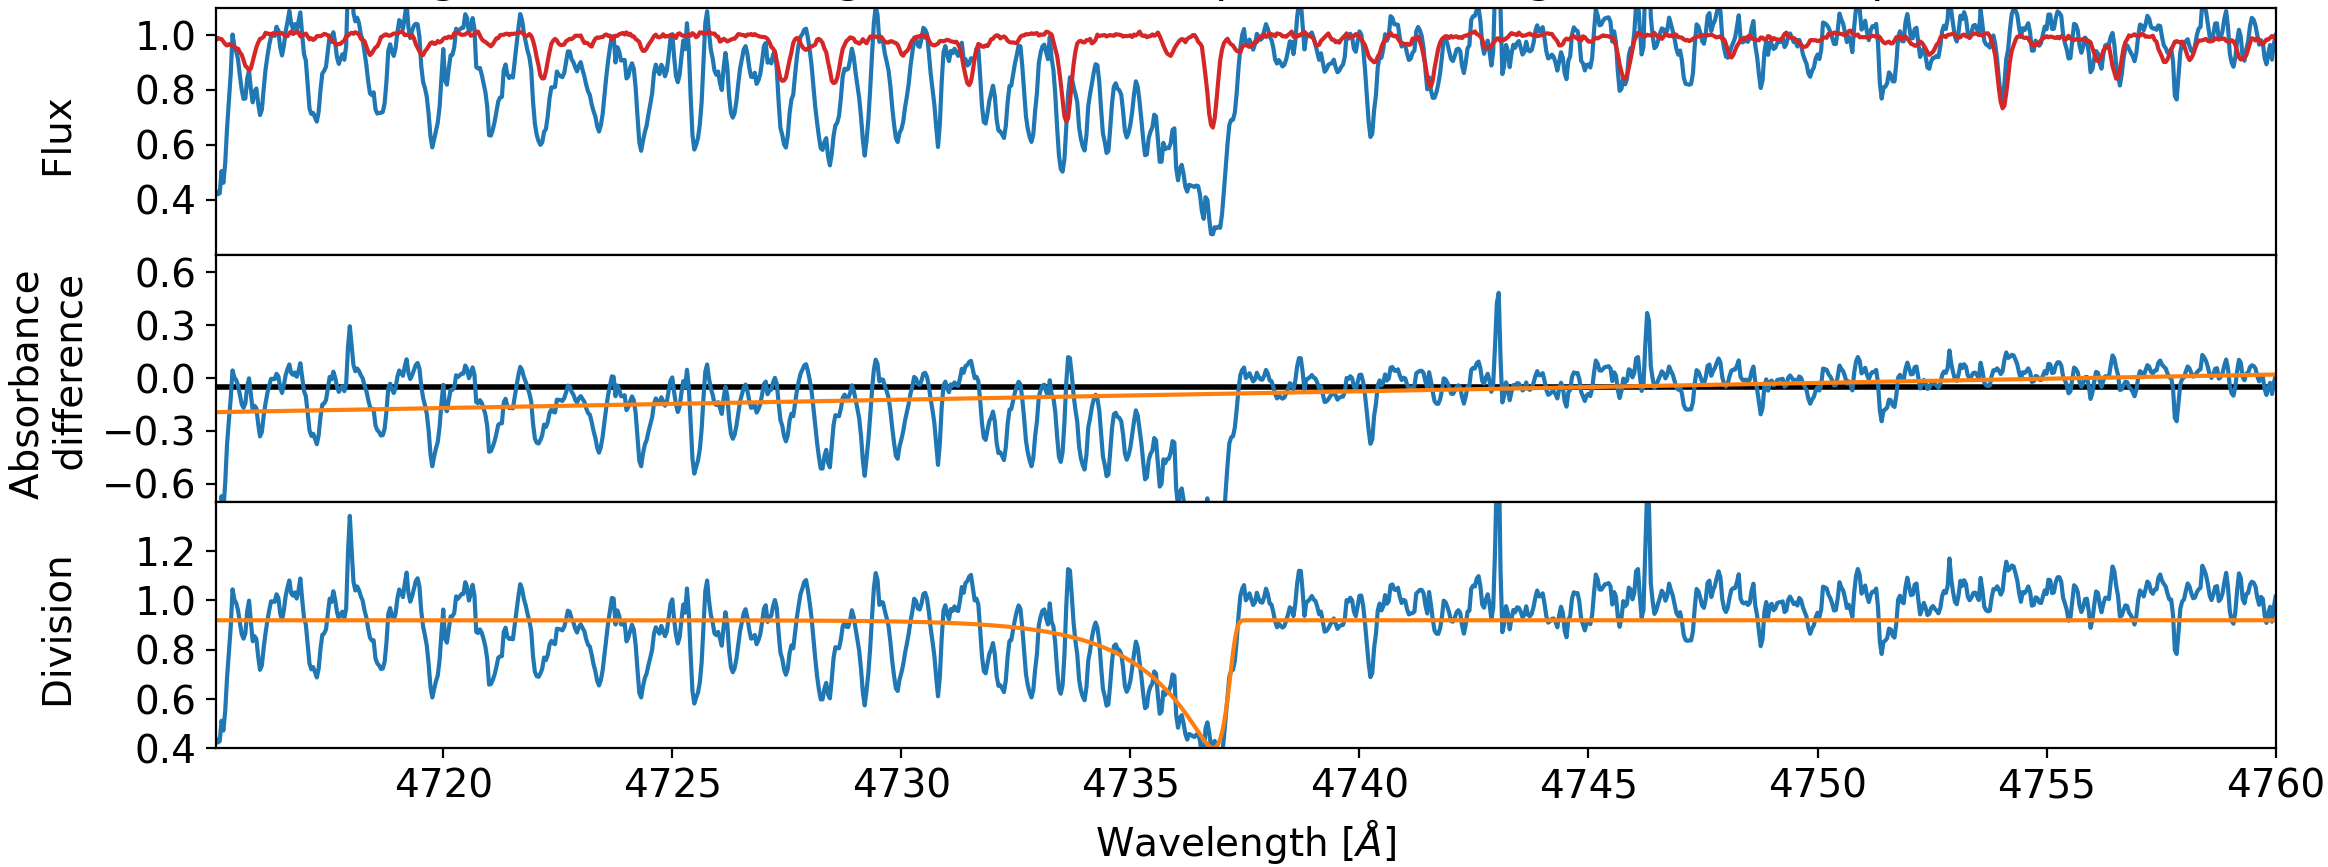
\includegraphics[width=\textwidth]{cemp_cand_150412003601009.png}
	\caption{Example of a metal-poor carbon-enhanced candidate with strong Swan absorption feature at 4737~\AA, caused by the carbon C$_2$ molecules. The first panel shows the stellar spectrum in blue and a corresponding reference median spectrum in red. The reference median spectrum was computed as the per-pixel median flux value of spectra with similar stellar parameters as the spectrum shown in blue. The spectral difference (second panel) and division (third panel) were computed from those two spectra. The middle panel shows in orange a linear fit to the spectral difference that was used to identify spectra with the reduction problems on the blue border of the spectral range. The median value of the spectral difference is given by the black horizontal line. The orange curve in the last panel shows a fit that was used to determine the strength of the observed carbon feature. The shown spectrum belongs to a star with a Two Micron All-Sky Survey (2MASS) identifier J11494247+0051023 and iron abundance \Feh\ of $-1.17$, as determined by \TC.}
	\label{fig:carbon_example}
\end{figure*}

\subsection{Supervised classification}
\label{sec:supervised}
To search for additional absorption features that are usually not found in spectra of chemically normal stars, we first built a spectral library of median spectra based on a rough estimates of stellar physical parameters derived by the automatic reduction pipeline, described in detail by \citet{2017MNRAS.464.1259K}. The median spectrum for every observed spectrum in our data set was computed from physically similar spectra with stellar parameters in the range of $\Delta$\Teff=$\pm75$~K, $\Delta$\Logg=$\pm0.125$~dex and $\Delta$\Feh=$\pm0.05$~dex around the stellar parameters of the investigated spectrum. The median spectrum was calculated only for observed targets with at least 5 similar spectra in the defined parameter range and with minimal SNR=15 per resolution element, as determined for the blue spectral arm. All considered spectra were resampled to a common wavelength grid with 0.04~\AA\ wide bins and then median combined. The normalisation of the spectra along with the radial velocity determination and the corresponding shift to the rest frame was performed by the automatic reduction pipeline \citep{2017MNRAS.464.1259K}. We checked that spectral normalisation and radial velocity determination are adequate also for carbon-enhanced stars. The normalisation procedure is done using a polynomial of low-order that is not strongly affected by the Swan band features or similar spectral structures. The radial velocity of a star is determined as an average of radial velocities that were independently determined for the blue, green, and red spectral arm. If one of the arms has a radial velocity deviating for more than two times the difference between the other two, it is excluded from the average \citep[further details in][]{2017MNRAS.464.1259K}. Therefore the final velocity should be correct even if one of those arms contains features that are not found in the set of reference spectra used in the cross-correlation procedure.

With the limitation of at least 5 spectra used for the computation of the median spectrum, some possibly carbon-enhanced stars, could be excluded from the supervised classification. The final number of spectra analysed by this method was 558,053.

Spectra, for which we were able to determine the median spectrum of physically similar objects, were analysed further. In the next step, we tried to determine possible carbon enhancement by calculating a flux difference and flux division between the observed stellar and median spectra, as shown in Figure \ref{fig:carbon_example}.

In order to describe the position, shape, and amplitude of the Swan feature with its head at 4737~\AA, we fitted a function that is based on a Log Gamma ($\log{}\Gamma$) distribution. The distribution, with three free parameters, was fitted to the division curve, where the Swan feature is most pronounced. Division curve, shown in the bottom panel of Figure \ref{fig:carbon_example}, was computed by dividing observed spectrum with its corresponding median spectrum. The fitted function $f$ can be written as:
\begin{equation}
\centering
f(\lambda) = f_0 - \log{}\Gamma(\lambda, S, \lambda_0, A).
\label{equ:loggamma}
\end{equation}
The shape of the curve is defined by an offset $f_0$, shape parameter $S$, centre wavelength $\lambda_0$, and amplitude $A$ of $\log{}\Gamma$ distribution, where $\lambda$ represents rest wavelengths of the observed spectrum. This function was selected because of its sharp rise followed by the gradual descent that matches well with the shape of a residual absorption observed in the Swan regions. The steepness of the rising part is determined by the parameter $S$ (lower value indicates steeper raise) and its vertical scaling by the parameter $A$. We are not aware of any other profile shapes used for fitting Swan bands in the literature.

To narrow down possible solutions for the best fitting curve, we used the following priors and limits. The initial value for the parameter $f_0$ was set to a median of all pixel values in the division curve and allowed to vary between $0.5$ and $1.5$. The limiting values are however newer reached. The centre of the $\log{}\Gamma$ distribution $\lambda_0$ was set to $4737$~\AA\ and was allowed to vary by $2$~\AA. Wavelength limits were set to minimise the number of mis-fitted solutions, where the best fit would describe the nearby spectral absorption lines not present in the median spectra or problematic spectral feature caused by the spectral data reduction as shown by Figure \ref{fig:bad_fit1}. We did not set any limits on parameters $A$ and $S$ in order to catch fitted solutions describing a spectrum difference that is different from the expected shape of the molecular absorption band.

\begin{figure*}
	\centering
	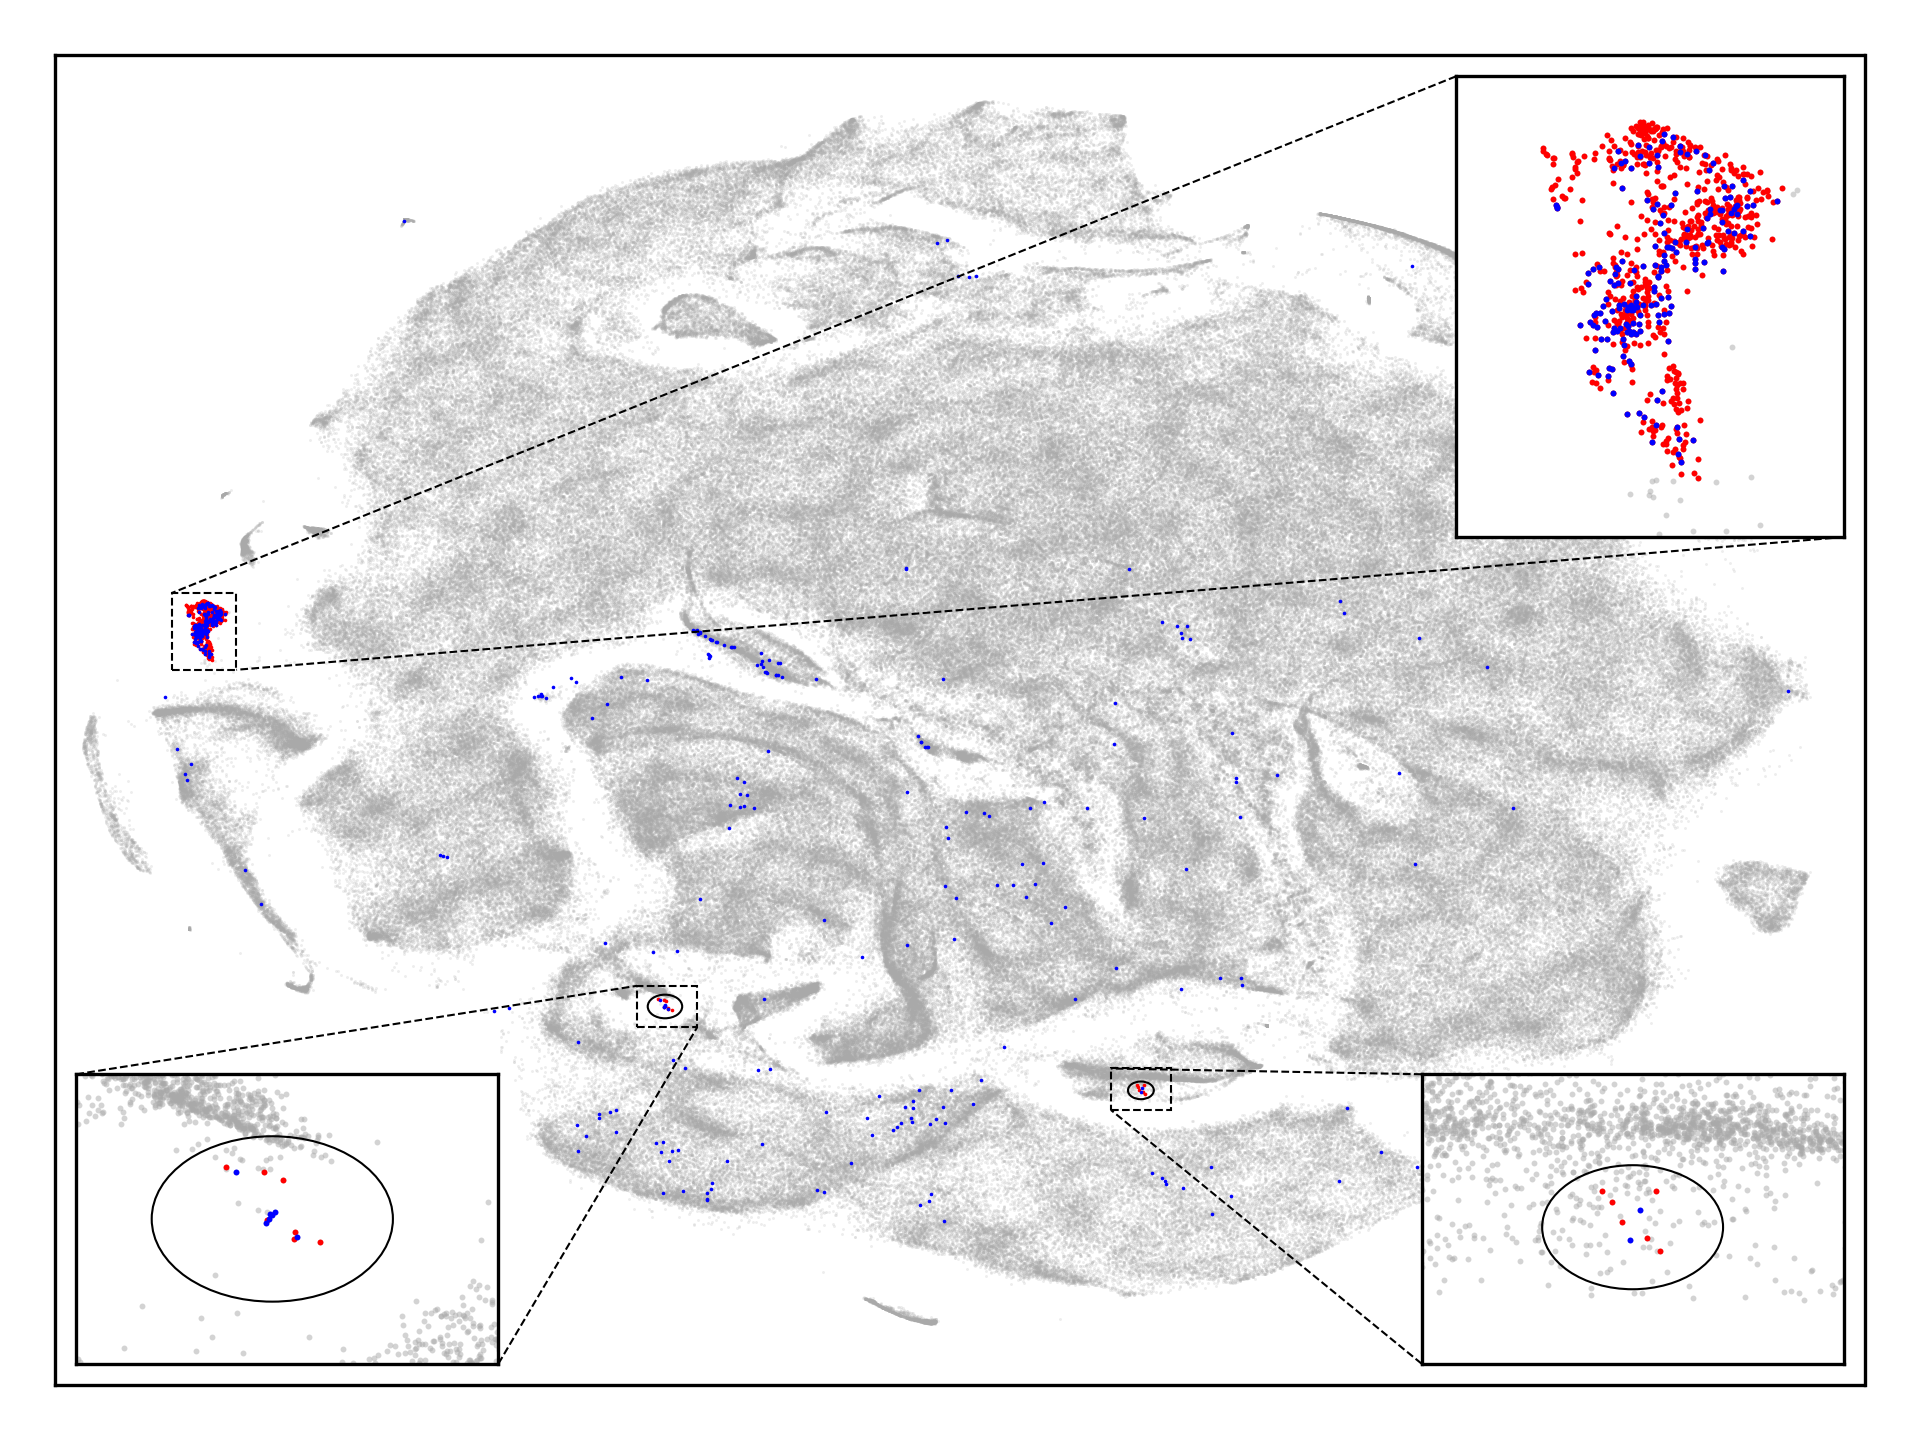
\includegraphics[width=\textwidth]{tsne_circles.png}
	\caption{t-SNE projection of 588,681 observed spectra ranging between 4720 and 4890~\AA. Red dots (756 spectra) mark a clump in the projection that was manually selected to contain carbon-enhanced spectra. Superimposed blue dots represent carbon-enhanced spectra determined by the supervised algorithm. Outside the t-SNE selected clump, we have 224 spectra that were determined to be carbon-enhanced only by the supervised method. All other analysed spectra are shown in grey shades, depending on their density in the 2D projection. Two ellipses indicate regions where the majority of CEMP candidates is located in the projection.}
	\label{fig:tsne_plot}
\end{figure*}

By integrating the surface between the offset $f_0$ and the fitted curve we calculated the strength of the Swan band. The integral (\texttt{swan\_integ} in Table \ref{tab:out_table}) is derived between 4730 and 4738~\AA. It should not be used as a substitute for a carbon abundance measurement, but only to sort the detections of carbon-enhanced stars by their perceivable strength of the Swan band.

With so many spectra in our data set, unexpected reduction and analysis problems can hinder the selection of carbon-enhanced stars. In the first iteration, the results were ordered only by the value of the integrated Swan band region, but this proved to select too many spectra with reduction problems. Most of the problematic detections were caused by the incorrect normalisation of spectra with strong, non-carbon molecular bands. This is best observable at the border of a spectral range, where Swan bands are located in the case of HERMES spectra. There, normalisation can be poorly defined in the case of numerous nearby absorption lines. In order to prevent miss-detections, additional limits on the shape ($S <= 1$) and amplitude ($A <= 1$) of the $\log{}\Gamma$ distribution were used to filter out faulty fitting solutions. Figure \ref{fig:bad_fit2} represents one such example where the function $f(\lambda)$ was fitted to the absorption lines of a double-lined spectroscopic binary, producing a shape of the function that is not characteristic for the analysed molecular band head. To remove spectra with reduction problems or peculiarity that would result in wrongly determined strength of the Swan band, we are also analysing the slope of the spectral difference and its integral in the limits of the Swan bands. One of the spectral trends that we are trying to catch with those indicators is shown in Figure \ref{fig:bad_fit2}, where spectral difference and its linear fit are steeply rising at the border of the spectrum.

By visual inspection of the algorithm diagnostic plots shown in Figure \ref{fig:carbon_example}, we limited a final selection to 400 spectra with the strongest carbon enhancement that was still visually recognisable. The last selected spectrum is shown in the Figure \ref{fig:carbon_last_supervised}. Selection of spectra with lower enhancement, would introduce possibly wrong classification of stars whose enhancement is driven by spectral noise levels, data reduction or any other process that has subtle effect on the spectral shape.

\subsection{Unsupervised classification}
\label{sec:unsupervised}
With numerous spectra of different stellar types, chemical composition, and degree of carbon enhancement, some of them might show different carbon features or be insufficiently distinctive to be picked out by the above supervised algorithm.

Another analysis technique, which is becoming increasingly popular is a dimensionality reduction procedure named t-distributed Stochastic Neighbor Embedding \citep[t-SNE,][]{van2008visualizing}, that has already proved to be beneficial in comparison and sorting of unknown spectral features of the same data set \citep{2017ApJS..228...24T}. This is done by projecting the complete spectra onto a 2D plane by computation of similarities between all pairs of investigated spectra. It has been shown that the algorithm can cluster and distinguish spectra with absorption or emission features. The algorithm arranges spectra in a 2D plane, such that it clusters similar spectra together based on their similarity measure. As the transformation is variable and non-linear, the actual distance between two objects in a final 2D plane does not linearly depend on the spectral similarity measure. This property of the t-SNE algorithm ensures more homogeneous coverage of the 2D plane in comparison to other dimensionality reduction methods.

The t-SNE projection shown in Figure \ref{fig:tsne_plot} was computed from normalised spectra between 4720 and 4890~\AA. To maximise the number of analysed spectra, no other limiting cuts than the validity of the wavelength solution \citep[bit 1 in \texttt{red\_flag} set to 0 by reduction pipeline, ][]{2017MNRAS.464.1259K} in this arm was used. This resulted in 588,681 individual spectra being analysed by the automatic unsupervised algorithm. This is $\sim30$k more spectra than in the case of supervised classification, where we applied more strict criteria for the selection of analysed spectra (Section \ref{sec:supervised}). 

Without any prior knowledge about the location of objects of interest in the obtained projection, we would have to visually analyse every significant clump of stars in order to discover whether the carbon-enhanced population is located in one of them. This can be simplified by adding the results of the supervised classification into this new projection. In Figure \ref{fig:tsne_plot}, the stars identified by the supervised classification are shown as blue dots plotted over grey dots representing all spectra that went into the analysis. The majority of blue dots are located in a clump on the left side of the projection. A high concentration of objects detected by a supervised method leads us to believe, that this isolated clump represents carbon-enhanced objects in the t-SNE projection. To select stars inside the clump, we manually drewn a polygon around it.

Inspection of other blue labelled spectra outside the main clump revealed that their slight carbon enhancement could not be identified by the t-SNE similarity metric as the spectra comparison might have been dominated by another spectral feature.

Additional exploration of the t-SNE projection revealed two smaller groups of metal-poor carbon-enhanced spectra located inside ellipses shown in Figure \ref{fig:tsne_plot}. A confirmation that those regions are populated with metal-poor stars can be found in Figure \ref{fig:tsne_teff_feh} where the dots representing spectra in the projection are colour coded by \Feh\ and \Teff. To maximise the number of those objects in the published catalogue, we manually checked all undetected spectra in the vicinity of the detected ones. This produced additional 13 CEMP detections.

\subsubsection{t-SNE limitation}
\begin{figure}
	\centering
	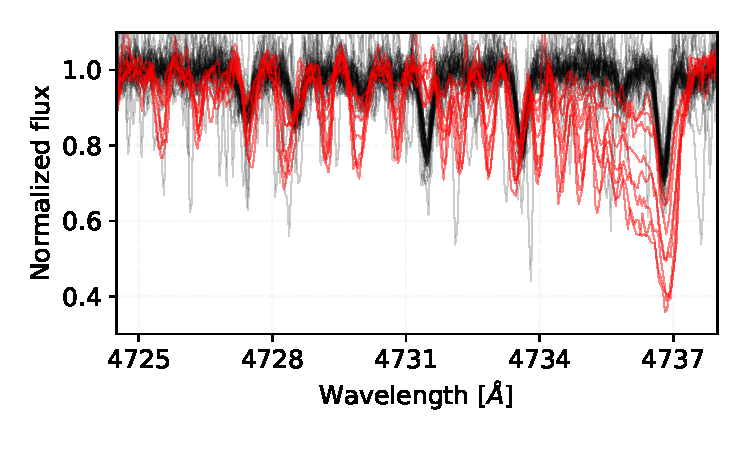
\includegraphics[width=\columnwidth]{tsne_cemp.pdf}
	\caption{A collection of spectra that were determined to be mutually very similar by the t-SNE algorithm. Out of 46 spectra inside the right black ellipse in Figure \ref{fig:tsne_plot} we identified 8 carbon-enhanced spectra with visually very different and distinctive spectrum in the region from 4734 to 4737~\AA\ that is also depicted in this figure. For easier visual recognizability, they are coloured in red.}
	\label{fig:tsne_cemps}
\end{figure}
While checking the local neighbourhood of some of the blue dots in Figure \ref{fig:tsne_plot} that are strewn across the t-SNE projection we identified a possible limitation of our approach for the automatic detection of specific peculiar spectra if their number is very small compared to the complete data set. Figure \ref{fig:tsne_cemps} shows a collection of a few carbon-enhanced spectra embedded between other normal spectra that were taken out of the right ellipsoidal region in Figure \ref{fig:tsne_plot}. As they are quite different from the others they were pushed against the edge of a larger cluster in the projection, but their number is not sufficient to form a distinctive group of points in the projection. Therefore any automatic algorithm that would try to distinguish those objects based solely on a local density of points would most probably fail.

Another specific of the t-SNE projection that we must be aware of is how it computes the similarity between analysed spectra. Combined similarity, which is computed as a sum of per pixel differences, has zero knowledge about the location where in the spectrum those differences occur. The red spectrum in Figure \ref{fig:tsne_30close} with a slight signature of carbon enhancement in the range between 4734 and 4737~\AA\ has been placed among spectra with similar physical properties. Its slight carbon enhancement and comparable spectral noise to other spectra in its vicinity are probably the reason why it was placed in such a region of the t-SNE projection. This could be solved by using a smaller portion of the spectrum in a dimensionality reduction, which could at the same time lead to a loose of other vital information about a star.

\begin{figure}
	\centering
	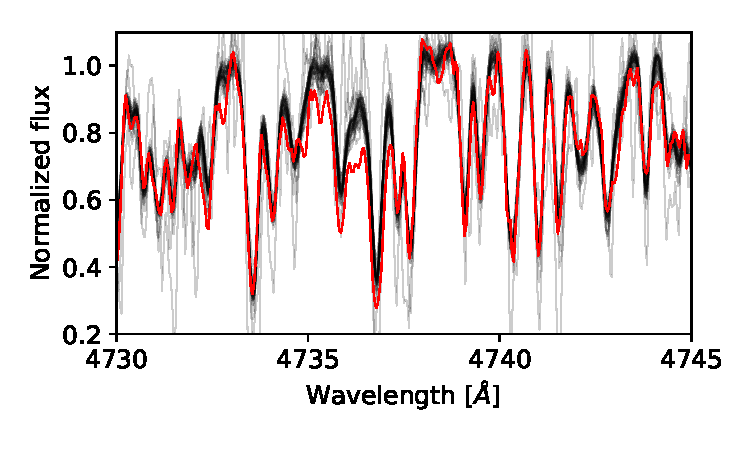
\includegraphics[width=\columnwidth]{150206004301057_tsne_close30.pdf}
	\caption{Spectral comparison between one of the detected carbon-enhanced stars in red and its 30 closest neighbours in the t-SNE projection shown as black curves. Enhancement in the spectrum was probably not sufficiently distinct and was dominated by the spectral noise. Therefore the spectrum was placed among other physically similar spectra without visible enhancement.}
	\label{fig:tsne_30close}
\end{figure}

\section{Candidate characteristics}
\label{sec:analysis}
The final list of detected carbon-enhanced stars consists of 918 stars, corresponding to 993 spectra detected by at least one of the described methods. Among them, 63 stars were observed and identified at least twice and up to a maximum of four times. Those identifications belong to repeated observations that were performed at different epochs. Because not all of the observed spectra were considered in the classification procedure (due to the limitations described in Section \ref{sec:classification}) this is not the final number of stars with repeated observations. By searching among the complete observational data set, the number of carbon-enhanced stars with repeated observations increases to 90.

Out of those 90 stars, every repeated observation of 56 stars was classified as being carbon-enhanced. In total, we detected $76.5$~\% of the carbon-enhanced spectra among repeated observations where at least one of the repeats have been classified as having enhanced carbon features in its spectrum. The unclassified instances usually have a low SNR value that could decrease their similarity value towards other carbon-enhanced stars in the t-SNE analysis or have incorrect stellar parameters and were therefore compared to an incorrect median spectra during the supervised analysis.

\subsection{Radial velocity variations}
\label{sec:binaries}
With repeated observations in the complete observational data set, we can look into measured radial velocities and investigate a number of possible variables that should be high for certain types of carbon-enhanced objects \citep{2016ApJ...826...85S}. Taking into account all of the repeated observations in our data set and not just the repeats among the identified spectra, 52 out of 90 stars show a minimum velocity change of $0.5$~\kms (70 stars with minimum change of $0.25$ \kms) and a maximum of $45$~\kms in different time spans ranging from days to years. The detailed distribution is presented by Figure \ref{fig:rv_rep_dist}. That kind of change can hint at the presence of a secondary member or at intrinsic stellar pulsation \citep{2002AA...390..987B, 2010JApA...31..177L, 2012A&A...544A..10B}, as carbon-enhanced stars are found among all long period variable classes \citep[Mira, SRa, and SRb, ][]{2013A&A...553A..93B, 2014A&A...568A.100B}. Follow-up observations are needed to determine their carbon sub-class and subsequently the reason behind variations of radial velocity.

\begin{figure}
	\centering
	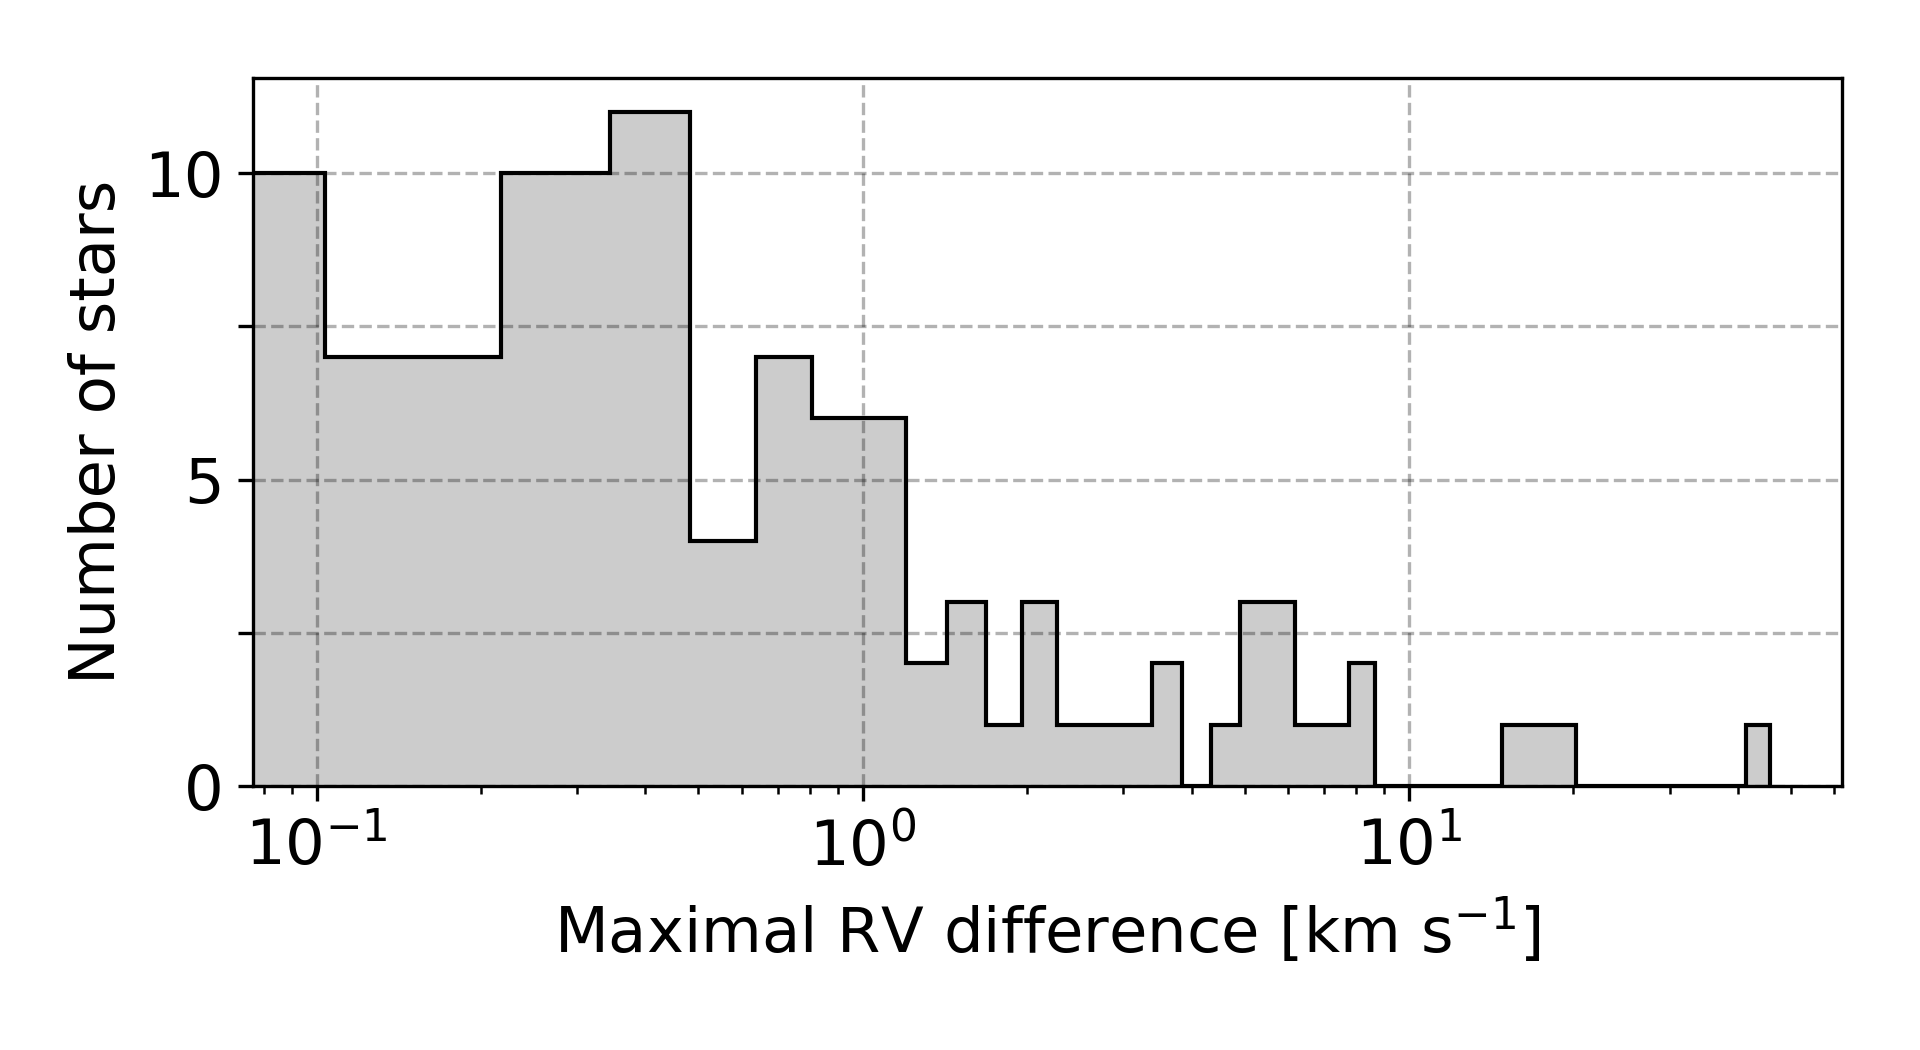
\includegraphics[width=\columnwidth]{rv_rep_dist.png}
	\caption{Distribution of maximal velocity change between repeated observations of the stars that were classified as carbon-enhanced.}
	\label{fig:rv_rep_dist}
\end{figure}

Visual inspection of variable candidates revealed that none of them shows obvious multiplications of absorption spectral lines, a characteristic of a double-lined binary system. Therefore we can conclude that none of them is a binary member in which both components are of comparable luminosity and a difference between their projected radial velocities is high enough to form a double-lined spectrum. From our simulations with median spectra, such line splitting becomes visually evident at the velocity difference of $\sim$14~\kms. If the components do not contribute the same amount of flux, the minimal difference increases to $\sim$20~\kms.

Chemical peculiarity of a dwarf carbon-enhanced star (dC) that exhibits enhancement of C$_2$ in its spectra could be explained by its interaction with a primary star in a binary system \citep{2018ApJ...856L...2M}. Chemically enhanced material is thought to be accreated from the evolved AGB companion. Less than thirty of such systems, that show signs of the existence of an invisible evolved companion who might have enriched a dC by the carbon, have been identified spectroscopically to date \citep{1986ApJ...300..314D, 2018ApJ...856L...2M, 2018MNRAS.479.3873W}, giving us the possibility to greatly increase the list with every additional confirmed object. The only detected dC star (for criteria see Section \ref{sec:cannon_params}) with repeated observations shows that its radial velocity is unchanged on the order of $0.1$~\kms\ during the 2 years between consecutive observations. Hence, it cannot be classified as a possible binary system from those two observations alone. The lack of a clear evidence for binarity among dC stars, especially among the most metal-poor, can also be explained by another enrichment mechanism. \citet{2018MNRAS.477.3801F} showed that a substantial fraction of those stars belongs to the halo population based on their kinematics information. Combined with the results of \citet{2016ApJ...833...20Y} that classified the prototype dC star \mbox{G 77-61} as a CEMP-no star, that are known to have intrinsically low binarity fraction \citep{2014MNRAS.441.1217S, 2016A&A...586A.160H}, their carbon-enhancement may be of a primordial origin.

\begin{figure}
	\centering
	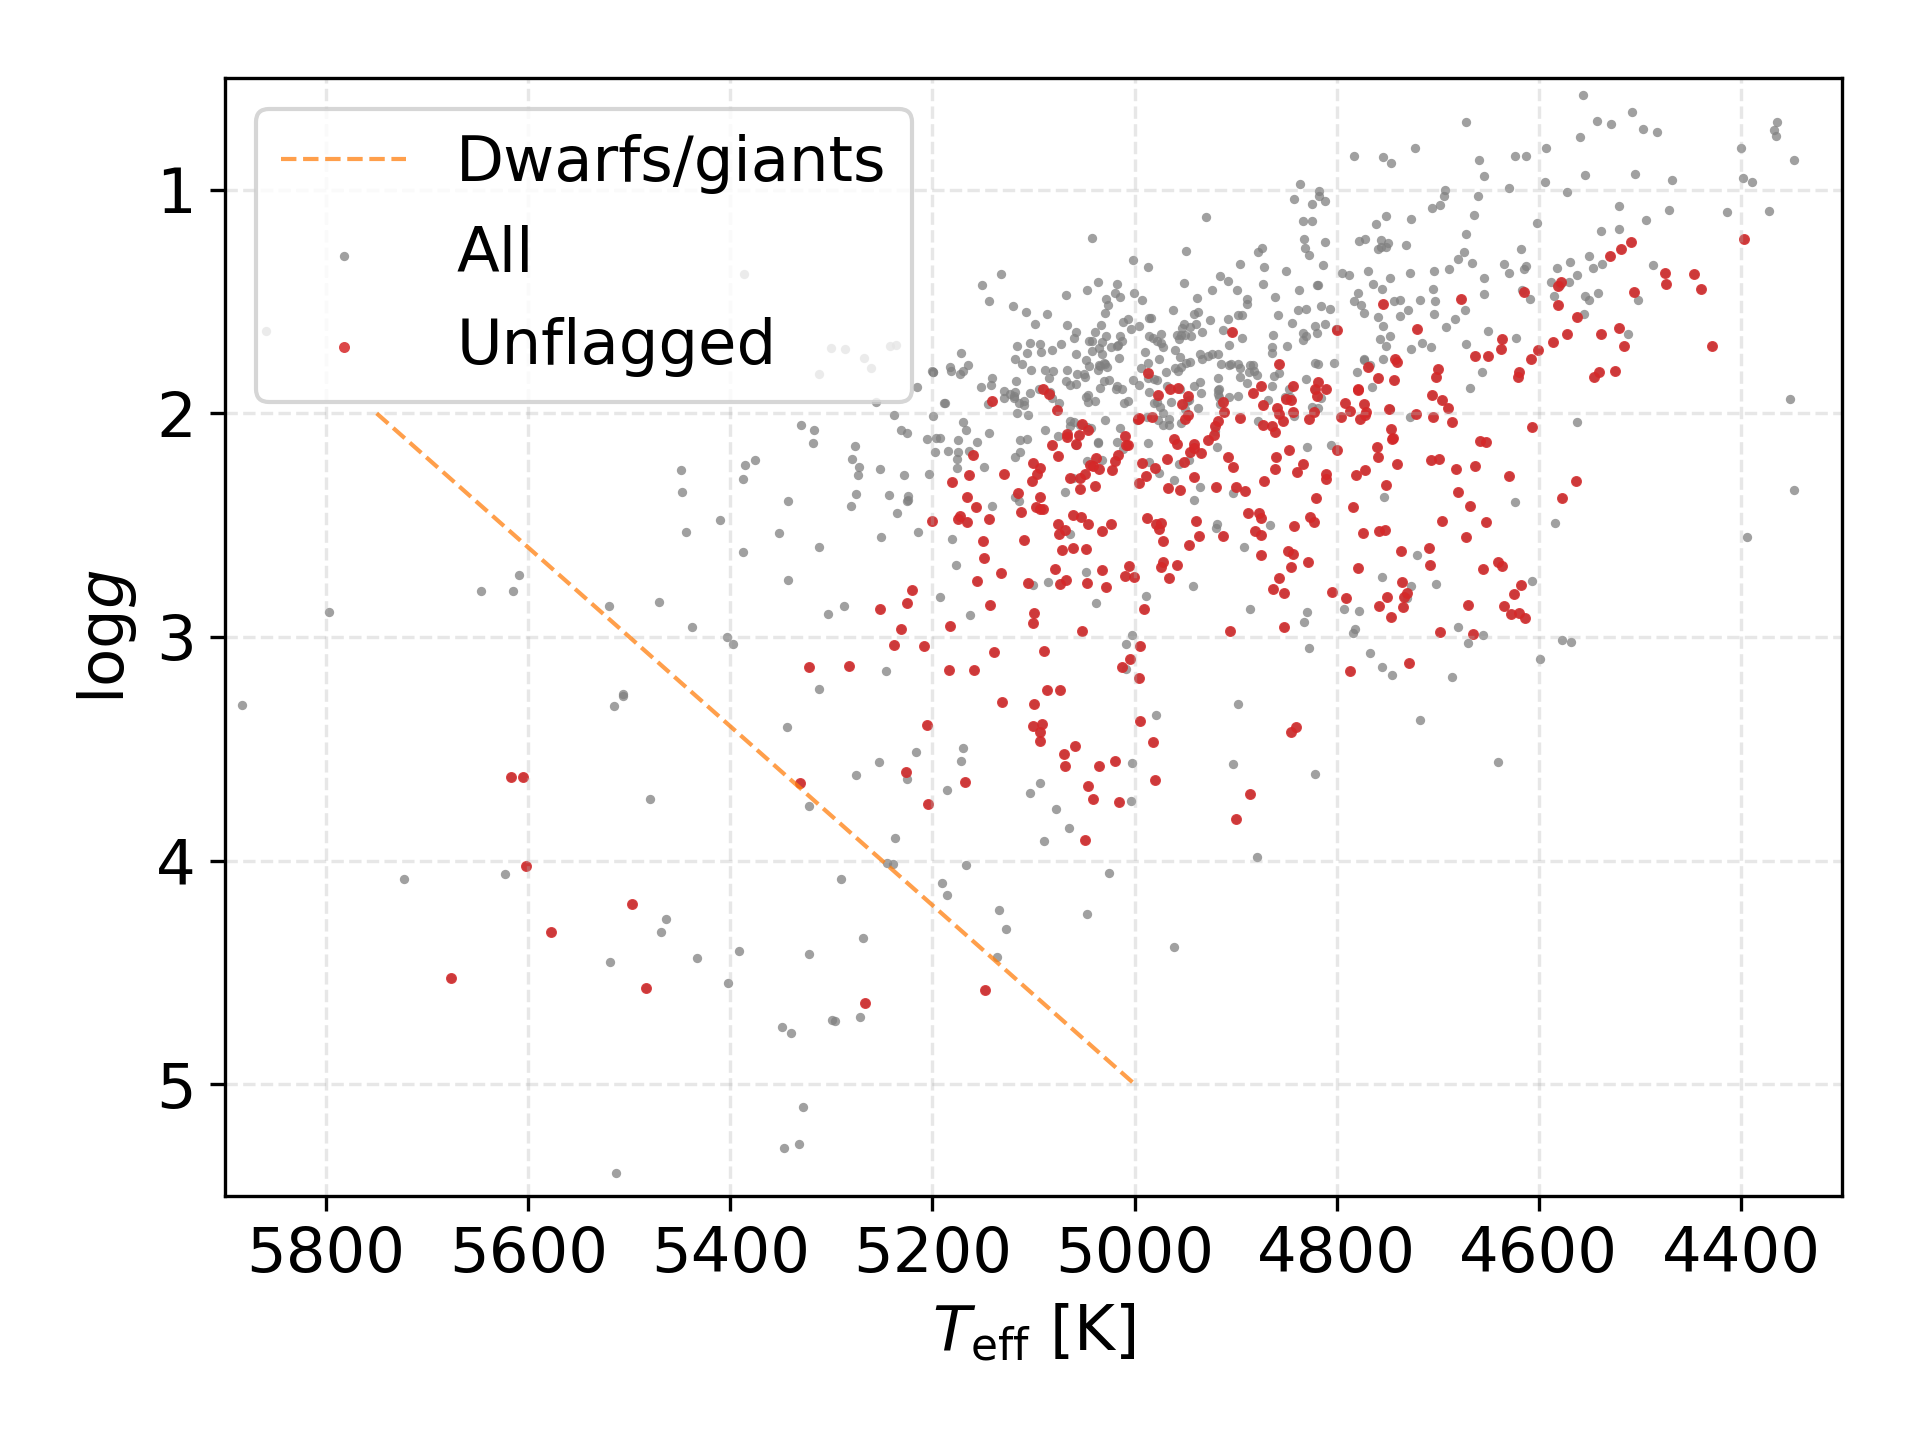
\includegraphics[width=\columnwidth]{Kiel_diagram.png}
	\caption{Kiel diagram for a subset of 338 detected carbon-enhanced stars with valid stellar parameters in red. Uncertain positions of flagged stars are shown with grey dots. Dashed orange line illustrates the border between giants and dwarfs.}
	\label{fig:kiel_plot}
\end{figure}

\subsection{Stellar parameters}
\label{sec:cannon_params}
For the analysis of stellar parameters, we used values determined by \TC\ data interpolation method that was trained on actual observed HERMES spectra. To exclude any potentially erroneous parameter, we applied a strict flagging rule of \texttt{flag\_cannon}=0 \citep[an extensive description of flagging procedure can be found in][]{buder2018}, thus obtaining a set of 347 objects with trustworthy stellar parameters. Such a large percentage of flagged objects could be attributed to their nature as an additional elemental enhancement that we are looking for might not be a part of the training set. A raised quality flag would hint that the spectrum is different from any other in the training set or that the fit is uncertain and has a large $\chi^2$. Therefore flagged parameters have to be used with care, especially on the border of, and outside the training set.

The majority (338) of the unflagged detected objects are giants and only 9 are confirmed to be dwarf stars based on their spectroscopic stellar parameters (Figure \ref{fig:kiel_plot}).

\begin{figure*}
	\centering
	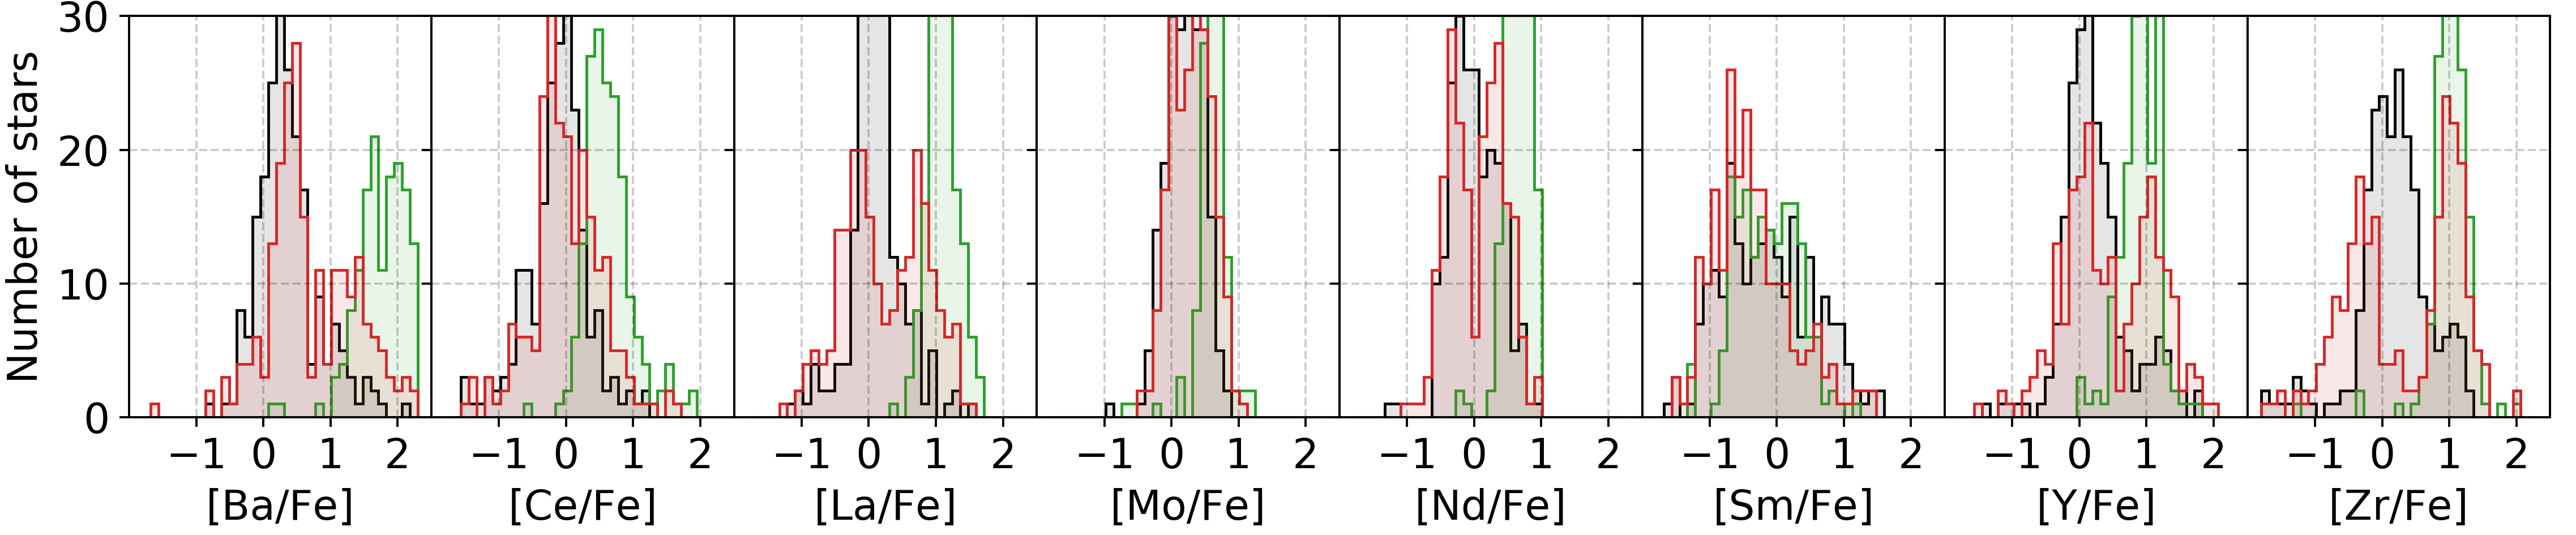
\includegraphics[width=\textwidth]{sprocess_hist.png}
	\caption{Distribution of s-process element abundances for stars in three different groups. The most enhanced group in green represent carbon-enhanced stars located in the t-SNE selected clump of stars. The red distribution presents all other detections that are placed around the projection, and outside the clump. As a control group, the same distribution in black is shown for their closest t-SNE neighbours, therefore the black and red distribution contain an equal number of objects. No abundance quality flags were used to limit abundance measurements.}
	\label{fig:sprocess_hist}
\end{figure*}

\subsection{S-process elements}
\label{sec:sprocess}
Focusing on a spectral signature of the detected objects inside and outside the t-SNE selected clump (Figure \ref{fig:tsne_plot}) we can further investigate which spectral feature might have contributed to their separation. The distributions of their abundances in Figure \ref{fig:sprocess_hist} and strength of spectral features corresponding to the same elements in Figure \ref{fig:sprocess_spectrum} hints to an enhancement of s-process elements among stars inside the selected clump. This additional enhancement might be another reason, besides the carbon enhancement, for the algorithm to cluster all of those stars as being different from the majority of spectra. 

\begin{figure}
	\centering
	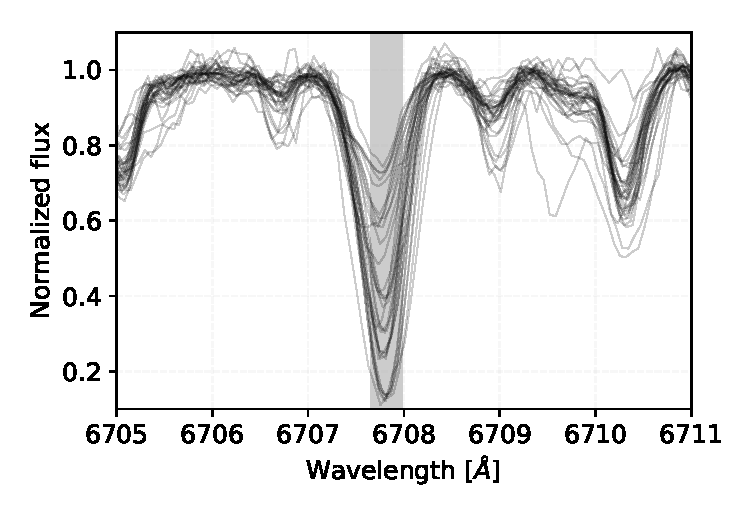
\includegraphics[width=\columnwidth]{li_string_ch.pdf}
	\caption{Spectral subset of 32 lithium-rich carbon-enhanced stars among the identified stars. The highlighted wavelength region is used by \TC\ to determine the lithium abundance of a star.}
	\label{fig:li_abund}
\end{figure}	

\subsection{Lithium abundance}
\label{sec:lithium}
The derivation of elemental abundances for known carbon-enhanced stars has shown that some of them can exhibit strongly enhanced levels of Li in their atmosphere \citep{1991A&A...245L...1A}. Lithium is thought to be produced by hot-bottom burning \citep{1974ApJ...187..555S} and brought to the surface from the stellar interior. Investigation of the Li line at 6707~\AA\ revealed 32 of such stars. Their spectra, centred around the Li feature, show a greatly varying degree of absorption in Figure \ref{fig:li_abund}.

\subsection{Sub-classes}
\label{sec:subclasses}
Following a revision of the original MK classification \citep{1941ApJ....94..501K} introduced by \citet{1996ApJS..105..419B}, carbon stars are separated into five different classes named \mbox{C-H}, \mbox{C-R}, \mbox{C-J}, \mbox{C-N}, and Barium stars. Of all the spectral indices proposed for the spectral classification, we are only able to measure a small part of Swan C$_2$ bands and Ba II line at 6496~\AA. For a more detailed classification of detected objects into proposed classes, we would need to carry out additional observations with a different spectroscopic setup to cover all the significant features. 

Additionally, the features caused by the $^{13}$C$^{12}$C molecule are strongly enhanced only for a handful of spectra in our data set, therefore we did not perform any isotopic ratio analysis or identification of possible C-J objects, which are characterised by strong Swan bands produced by the heavier isotopes.

According to the abundance trends presented in Section \ref{sec:sprocess} and the classification criteria defined by \citet{1996ApJS..105..419B}, we could argue that the stars selected from the t-SNE projection belong to the C-N sub-class. Their s-process elements are clearly enhanced over Solar values (Figure \ref{fig:sprocess_hist}), but the actual values should be treated with care as they are mostly flagged by \TC. This uncertainty might come from the fact that the training set does not cover carbon-enhanced stars and/or stars with such enhancement of s-process elements.

\subsection{Match with other catalogues}
In the literature we can find numerous published catalogues of carbon-enhanced (CH) stars \citep{2001A&A...375..366C, 2001BaltA..10....1A,2016ApJS..226....1J} and CEMP stars \citep{2007ApJ...658..367K, 2010A&A...509A..93M, 2010AJ....139.1051P, 2014ApJ...797...21P, 2015A&A...581A..22A, 2017yCat..18330020Y} observed by different telescopes and analysed in inhomogeneous ways. Most of those analyses were also performed on spectra of lower resolving power than the HERMES, therefore some visual differences are expected for wide molecular bands. By matching published catalogues with the GALAH observations that were analysed by our procedures, we identified 44 stars that matched with at least one of the catalogues. Of these, 28 were found in CH catalogues and 16 in CEMP catalogues.

From the stars recognised as CEMPs in the literature, we were able to recover only 1 of them. Visual assessment of the diagnostic plots provided by our analysis pipeline proved that the remaining 15 CEMP matches do not expresses any observable carbon enhancement in Swan bands and were therefore impossible to detect with the combination of our algorithms. The reason for this difference between our and literature results might be in the CEMP selection procedure employed by the aforementioned literature. Every considered study selects their set of interesting stars from one or multiple literature sources based on values of \Meh\ and \Cfe\ that were measured from the atomic spectral lines and not molecular lines. 

The match is larger in the case of CH matches, where we were able to confirm 11 out of 33 possible matched carbon-enhanced stars. As the observed molecular bands are prominent features in the spectra, we explored possible reasons for our low detection rate. Visual inspection of spectra for the remaining undetected matched stars proved that they also show no or barely noticeable carbon enhancement in the spectral region of Swan bands, therefore reason must lie in the detection procedures used in the cited literature. \citet{2001A&A...375..366C} used low-resolution spectra to evaluate enhancement of C$_2$ and CN bands. The results are also summarised in their electronic table. In here, all of our undetected stars are marked to contain enhanced CN bands but no C$_2$ bands. Combining this with Figure \ref{fig:ch_xmatch} we speculate that those stars occupy a narrow range of parameter space where C$_2$ is not expressed and therefore undetectable in the HERMES spectra. 

Number of successfully detected stars matched between the surveys could also be influenced by different excitation temperatures of analysed carbon-rich molecules. Frequently studied photometric G-band, that is not present in our spectra, covers a spectral region rich in CH molecule features whose temperature dependence is different than for a C$_2$ molecule. Presence of those bands is identified by classifying a carbon-enhanced star into C-H sub-class (see Section \ref{sec:subclasses}). As we detected all C-H stars identified by \citet{2016ApJS..226....1J}, that are also present in the GALAH data set, we are unable to discuss about the selection effect in the \Teff\ range between $\sim$5100 and $\sim$5300~K where those three stars were found.

\begin{figure}
	\centering
	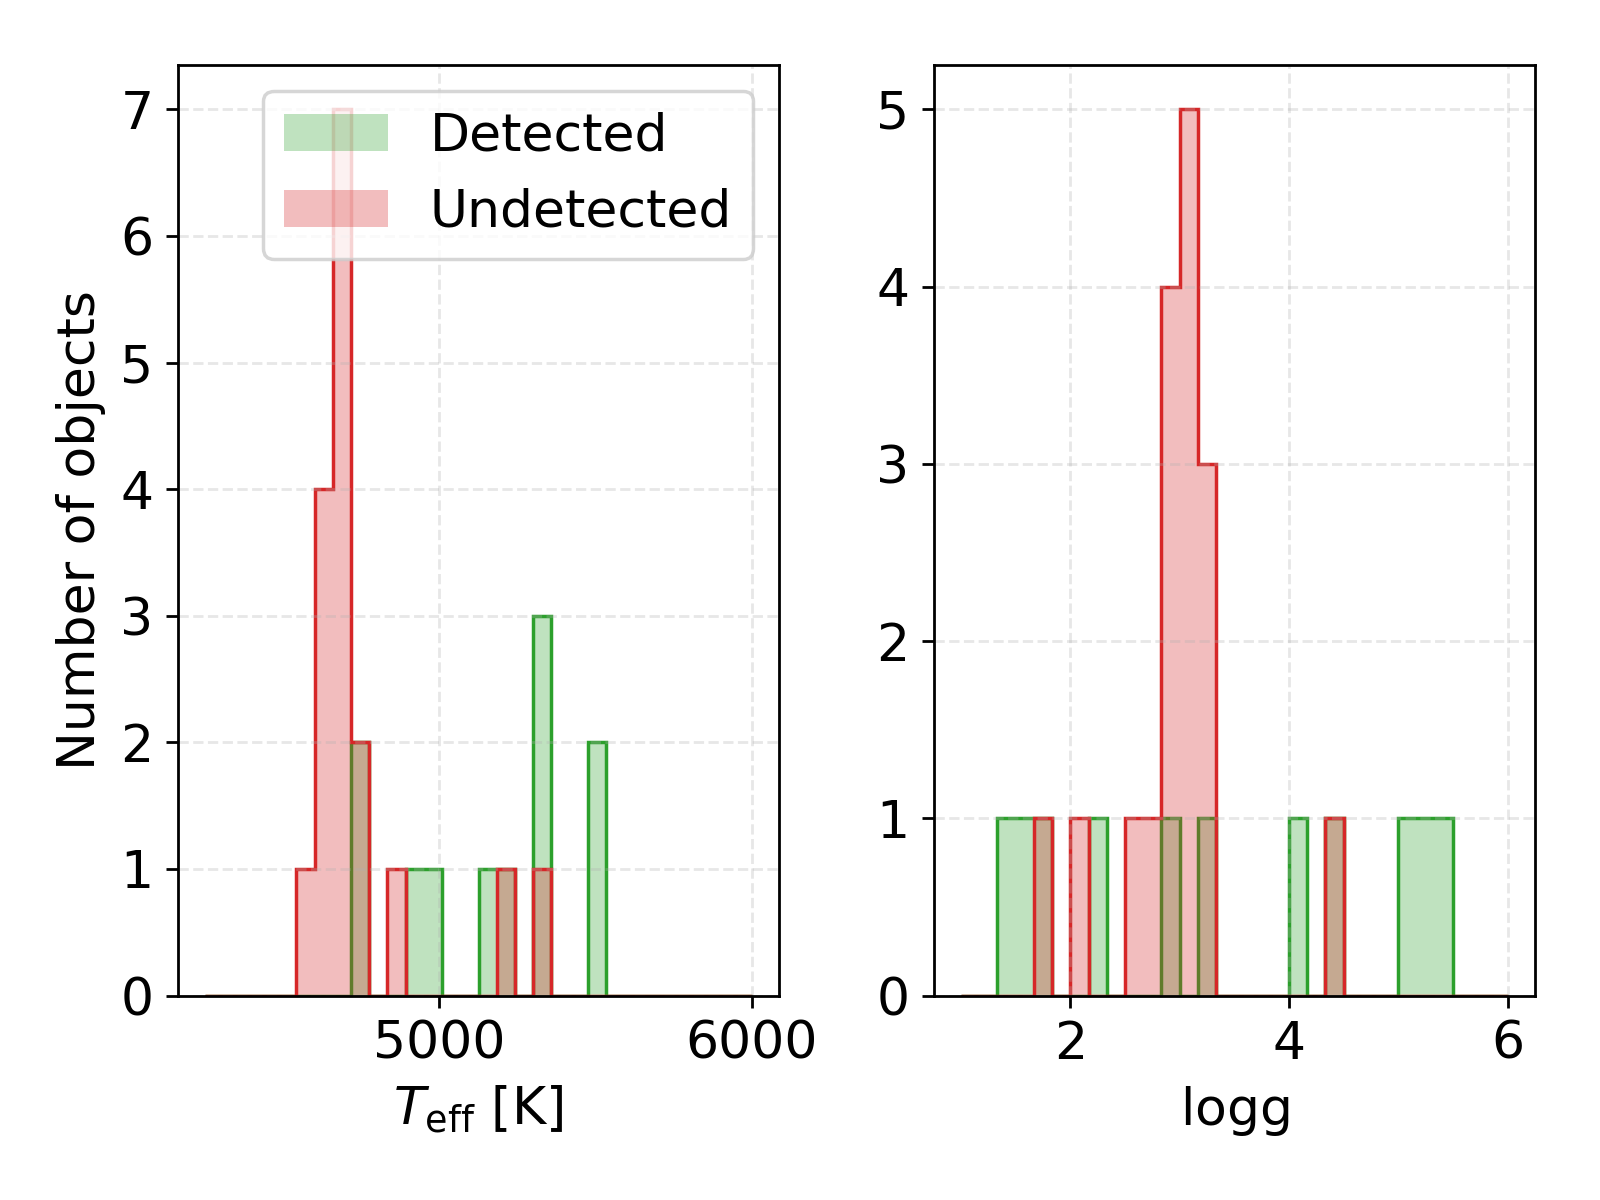
\includegraphics[width=\columnwidth]{ch_comb.png}
	\caption{Comparison between the stellar parameters of detected (green histogram) and undetected (red histogram) carbon-enhanced stars found in literature.}
	\label{fig:ch_xmatch}
\end{figure}

The position of all stars matched with the literature is also visualised on the \mbox{t-SNE} projection in Figure \ref{fig:tsne_ref_ch}, where it can be clearly seen that they lie outside the selected clump with identified carbon enhancement and are strewn across the projection. Close inspection of spectra that are spatially near the aggregation of CEMP stars from the literature, revealed no visible carbon enhancement. The enhancement is present neither in form of molecular bands nor expressed as stronger atomic carbon line. They therefore are indistinguishable from other metal-poor stars with similar physical parameters.

\begin{figure}
	\centering
	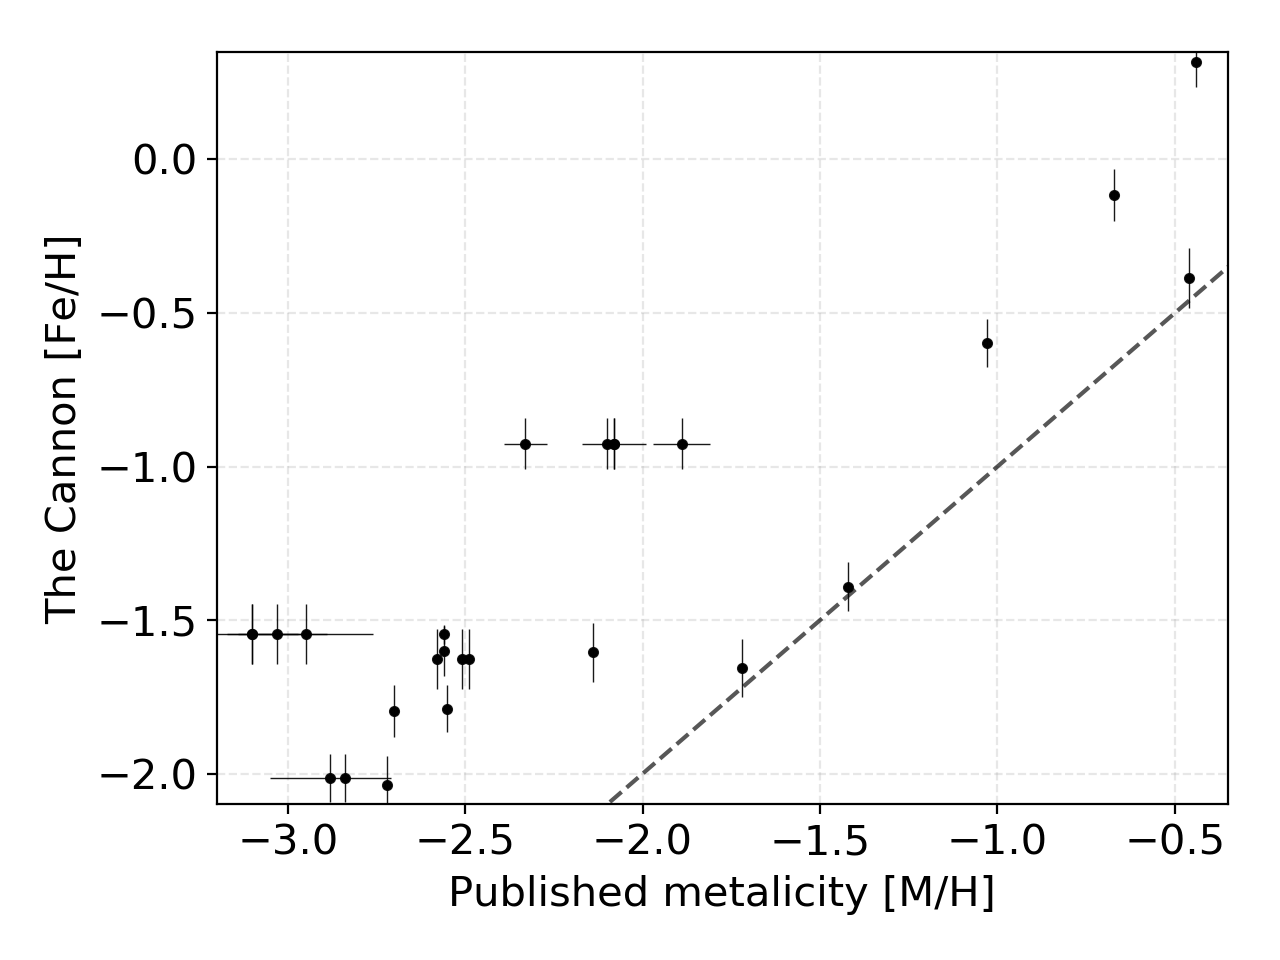
\includegraphics[width=\columnwidth]{cemps_meh_feh.png}
	\caption{Correlation between published metallicities and \TC\ iron abundance for the stars that were classified as CEMPs in the literature. As some of those stars were taken from multiple literature sources, we also have multiple determinations of \Meh\ for them. This can be identified as horizontal clusters of dots at different \Meh, but with the same \Feh. Where available, uncertainties of parameters are shown. The dashed line follows a 1:1 relation.}
	\label{fig:cemps_feh}
\end{figure}

\section{Metal-poor candidates}
\label{sec:cemp}
CEMP stars are defined in the literature as having low metallicity \Meh \textless $-1$ and strong carbon enrichment \Cfe \textgreater $+1$. In the scope of this analysis, we assume that our measurement of \Feh\ is a good approximation for the metallicity. To be sure about this we compared \Meh\ values of CEMP stars found in the literature and \Feh\ derived by \TC\ for the same stars. The relation between them is shown in Figure \ref{fig:cemps_feh}. We see that our values start deviating from the published values at metallicities bellow $-1.5$. Bellow that threshold the differences are in the range of $\sim1$ dex, but the same trend is obvious for both data sets. The uncertainty of the published \Meh, derived from multiple sources, can reach up to $0.5$. 

\begin{figure}
	\centering
	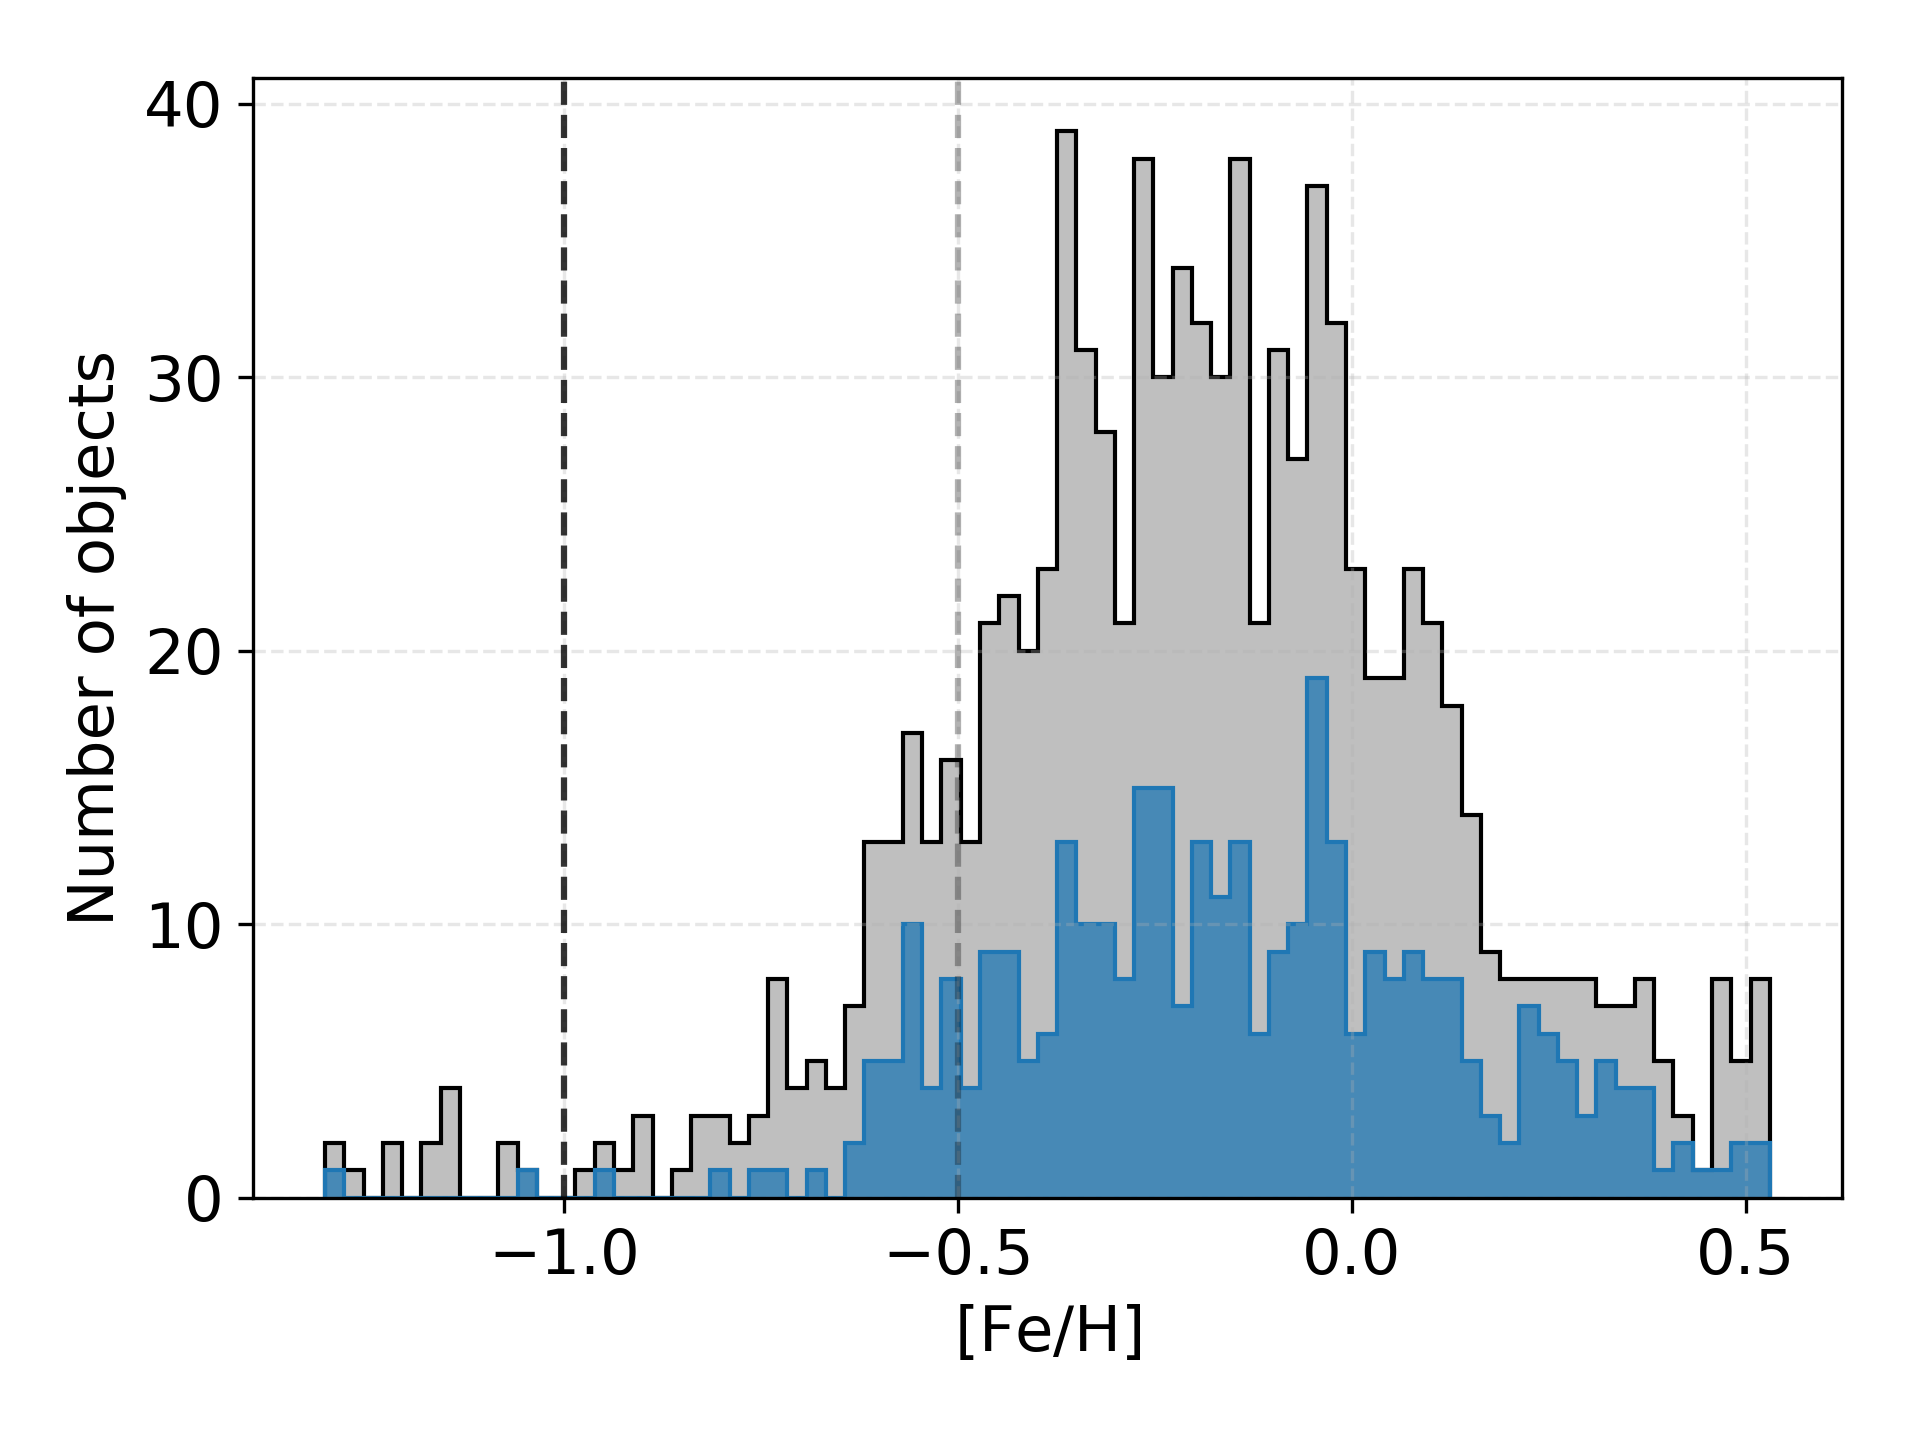
\includegraphics[width=\columnwidth]{Fe_H_cannon.png}
	\caption{Histogram of \Feh\ for detected carbon-enhanced stars with valid \TC\ stellar parameters in blue and for every detected carbon-enhanced star in grey. Two vertical lines are located at iron abundances of $-1.0$ and $-0.5$.}
	\label{fig:feh_candidates}
\end{figure}

Taking unflagged \TC\ parameters and abundances of the detected objects we can determine possible CEMP candidates among our sample. As also shown by Figure \ref{fig:feh_candidates} our set of carbon-enhanced stars consists of 41 objects with \Feh \textless $-0.5$ and 2 objects with \Feh \textless $-1.0$. If we also include potentially incorrect parameters, the number of objects with \Feh \textless $-1.0$ increases to 28, which is equal to $2.8$~\% of detected carbon-enhanced spectra. In any case, none of them has a valid determination of carbon abundance. Analysing HERMES spectra in order to determine carbon abundance is difficult because the automatic analysis is based on only one very weak atomic absorption line that is believed to be free of any blended lines. Consequently, we are also not able to measure the \CO\ abundance ratio, as a majority of determined \Cfe\ abundances is flagged as unreliable. Complementary observations are needed to determine the abundance and confirm suggested CEMP candidates.

A low number of metal-poor candidates could also be explained by the specification of the HERMES spectrograph as its spectral bands were not selected in a way to search for and confirm most metal-poor stars. With the release of {\it Gaia} DR2 data \citep{2018A&A...616A...1G}, stars low/high-metallicity could also be compared with their Galactic orbits. To determine the distribution of detected stars among different Galactic components, we performed an orbital integration in \texttt{MWPotential2014} Galactic potential using the \texttt{galpy} package \citep{2015ApJS..216...29B}. In order to construct a complete 6D kinematics information, {\it Gaia} parallax and proper motion measurements were supplemented with the GALAH radial velocities. Results shown in Figure \ref{fig:orbits_zmax} suggest that our CEMP candidates could belong to two different components of the Galaxy. Stars with maximal $z$~<~4~kpc most probably belong to the thick disk and stars with $z$~>~5~kpc to the halo population that is inherently metal-poor. This is also supported by their angular momentum in the same plot and their Galactic velocities shown in Figure \ref{fig:orbits_vxvyvz}.

When looking at the distribution of \Feh\ for the complete set of observed stars, we find a comparable distribution as for carbon-enhanced stars. Similarly, about $1.8$~\% of stars are found to be metal-poor with \Feh \textless $-1.0$.

\begin{figure}
	\centering
	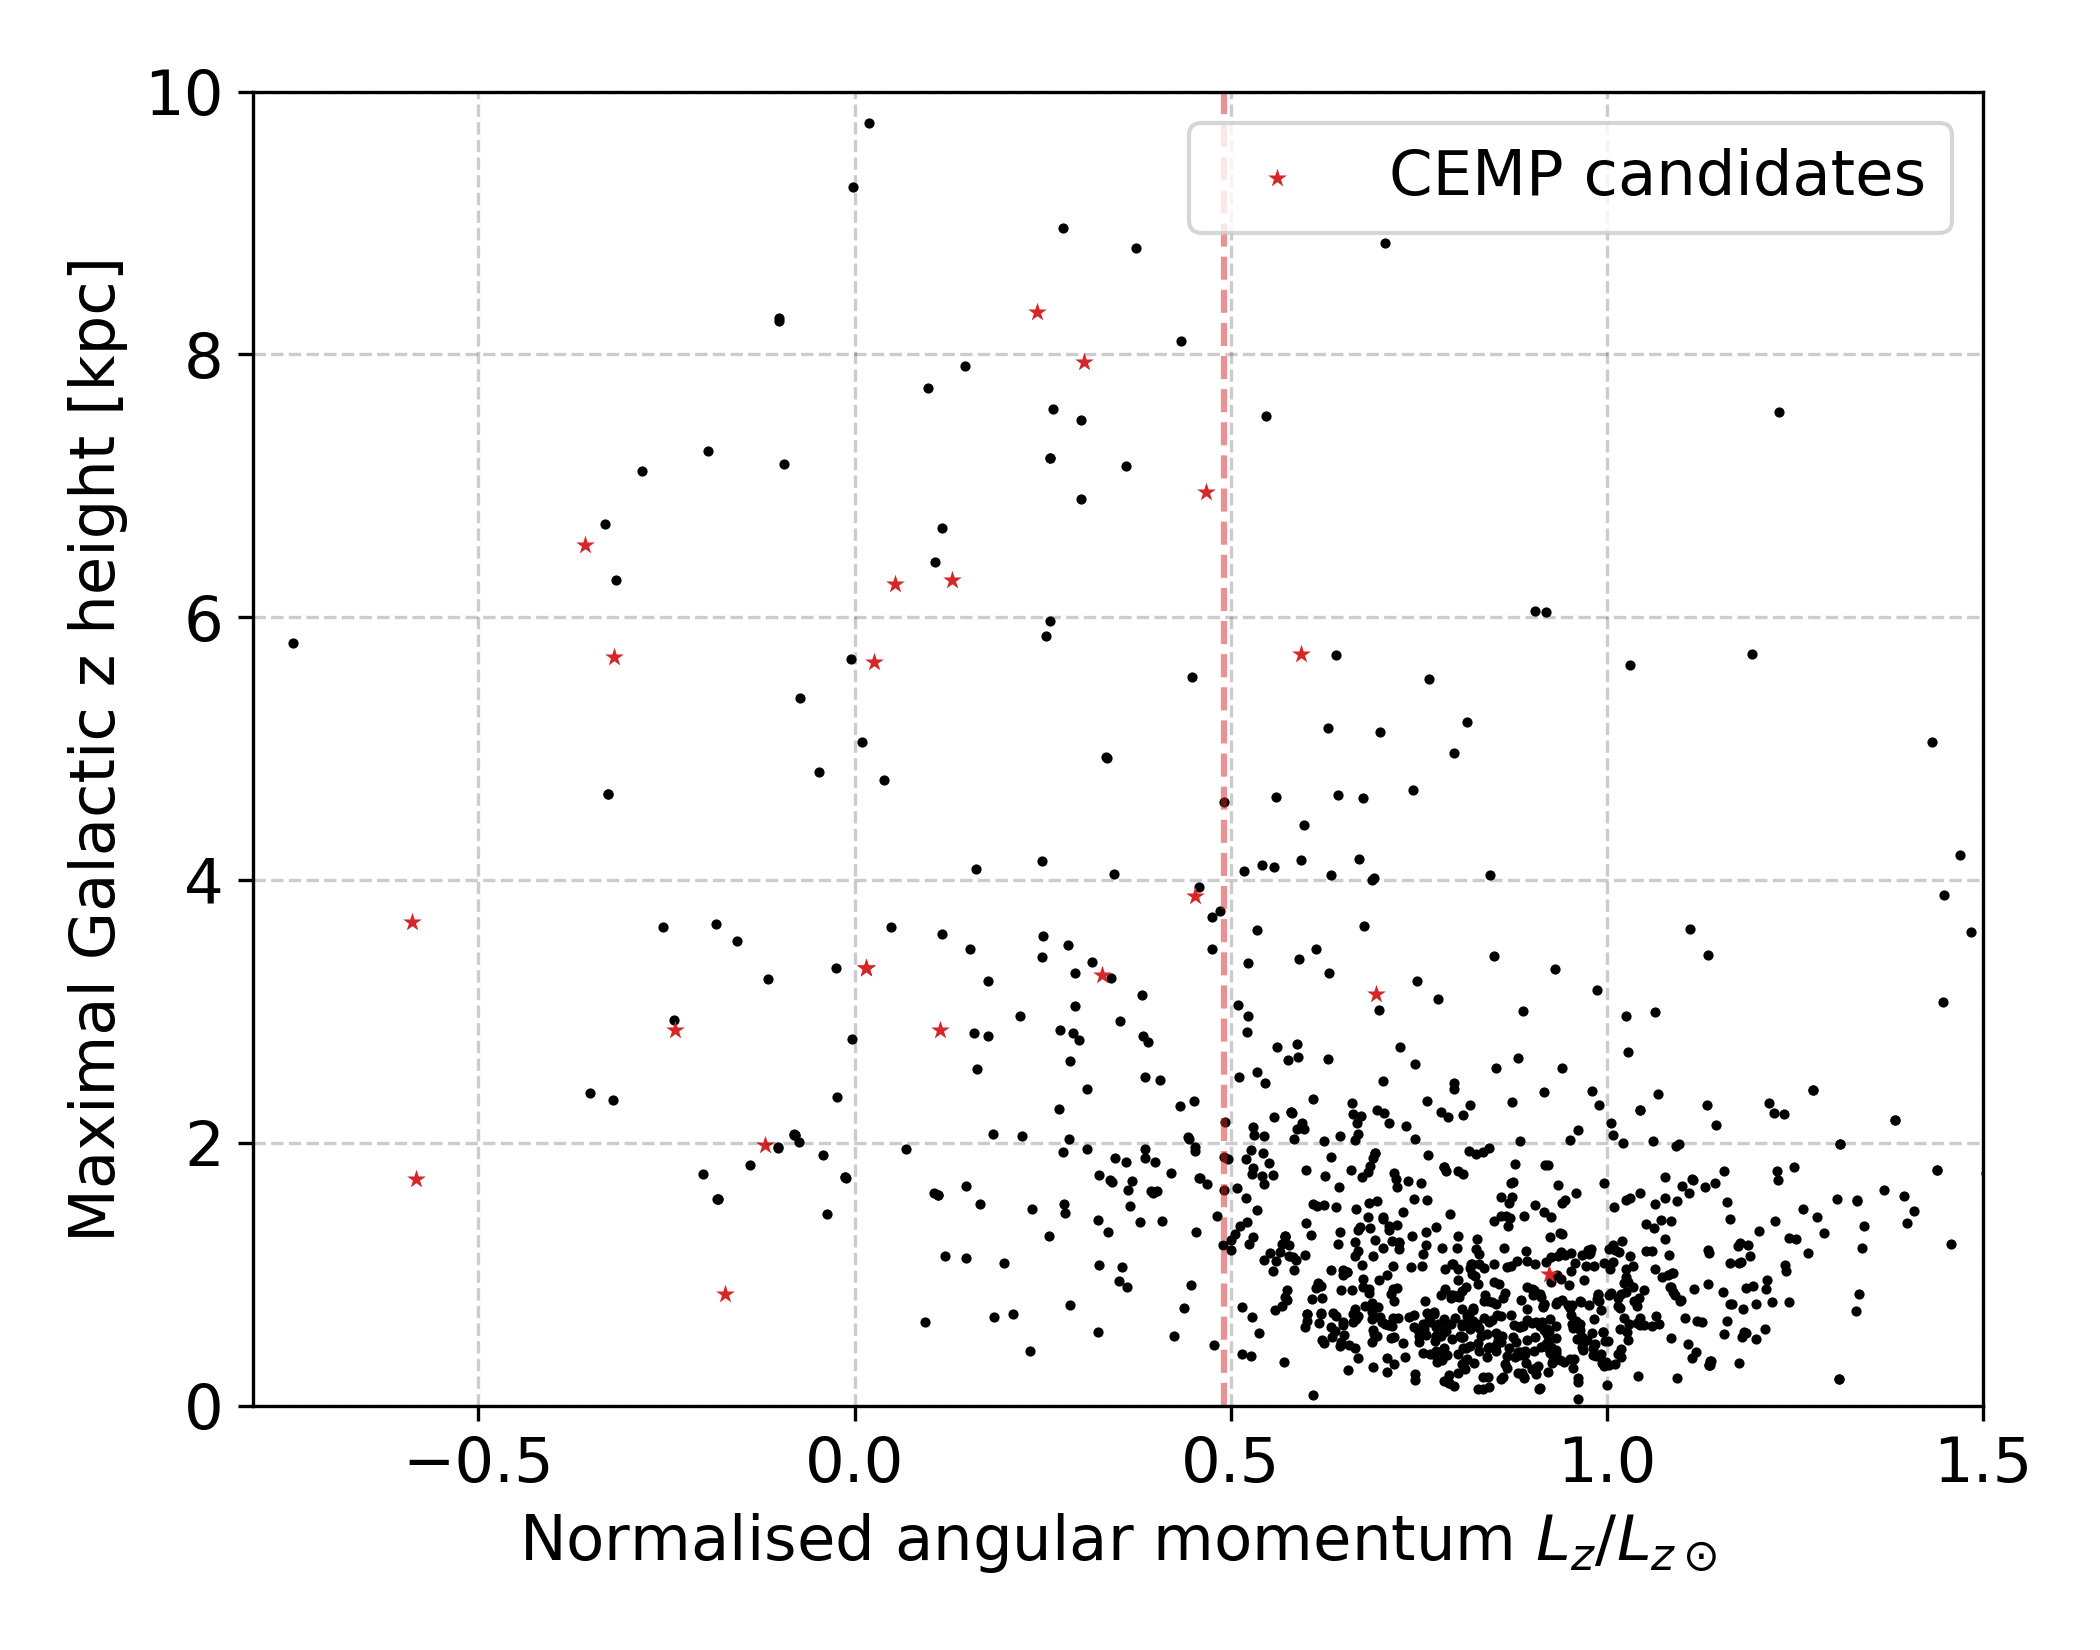
\includegraphics[width=\columnwidth]{carbon_orbits_zmax_lznorm.png}
	\caption{Distributions of maximal height above/below the Galactic plane reached by detected stars on their orbit around the centre of the Galaxy in comparison to their normalised angular momentum $L_z$. Vertical dashed line at $1000$~\kms~kpc highlights the transition from the halo to the disk population, where a majority of the halo stars is located below this threshold \citep[the threshold was visually estimated from similar plots in][]{2018ApJ...860L..11K}.  CEMP candidates are marked with star symbols.}
	\label{fig:orbits_zmax}
\end{figure}

\section{Follow-up observation}
\label{sec:asiago}

\begin{figure}
	\centering
	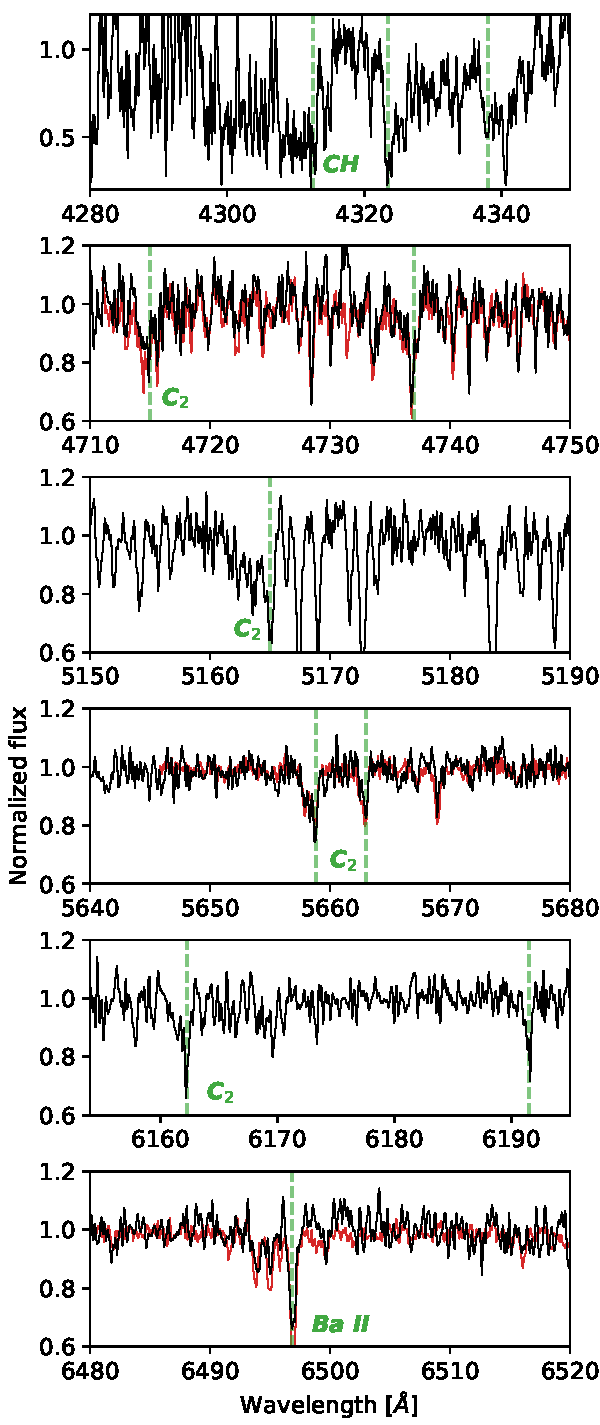
\includegraphics[width=\columnwidth]{asiago_cemp2.pdf}
	\caption{Subsets from the follow-up Asiago spectrum with resolving power comparable, but not identical, to the HERMES spectrum. It contains multiple spectral features used to evaluate carbon enhancement in a star and its carbon sub-class. Relevant spectral features are marked with vertical dashed green lines and labels that represent a molecule or element that is responsible for the features shown in the individual panel. The 2MASS identifier of the observed star is J11333341-0043060. In the wavelength ranges where it is available, the GALAH spectrum of the same star is shown in red.}
	\label{fig:asiago}
\end{figure}

To further classify and analyse one of the detected objects, a star with 2MASS identifier J11333341-0043060 was selected for a follow-up observation. We acquired its high-resolution Echelle spectrum (with the resolving power R $\sim 20,000$), using a spectrograph mounted on the $1.82$~m Copernico telescope located at Cima Ekar (Asiago, Italy). Because only a few of our detected candidates are observable from the Asiago observatory, we selected the best observable CEMP candidate, whose \Feh\ was determined by \TC\ to be $-0.96$. The selected star, with V = $12.79$, was on the dark limit of the used telescope, therefore low SNR was expected. The one-hour long exposure of the selected object was fully reduced, normalised order by order, and shifted to the rest frame.

Although the acquired spectrum covers a much wider and continuous spectral range (from 3900 to 7200~\AA) than the HERMES spectra, only subsets, relevant for the classification of carbon-enhanced stars are presented in Figure \ref{fig:asiago}. They were identified by visually matching our observed spectrum with the published moderate-resolution spectral atlas \citep{1996ApJS..105..419B} of peculiar carbon stars. Where available, the GALAH spectrum is shown alongside the Asiago spectrum. Carbon enhancement is not expected to vary over a period of several years, therefore both spectra should show similar features. The second and fourth panel in Figure \ref{fig:asiago} confirm that both observations indicate a similar degree of carbon enhancement.

Following the classification criteria of carbon stars, we determined that the star belongs to the C-H sub-class. The definitive features for this class are strong molecular CH bands, prominent secondary P-branch head near 4342~\AA\ (top panel in Figure \ref{fig:asiago}), and noticeable Ba II lines at 4554 and 6496~\AA\ \citep{2018ApJS..234...31L}, which are all present in the spectrum. The star definitely does not have a high ratio between $^{13}$C and $^{12}$C isotopes as the Swan features corresponding to $^{13}$C are clearly not present, therefore it can not be of a C-J sub-class.

Following the current state of knowledge \citep{1990ApJ...352..709M, 2016AA...586A.158J, 2016ApJ...826...85S} that most, if not all, C-H stars show clear evidence for binarity, we compared the radial velocity between both observations. They hint at the variability of the object as the follow-up radial velocity ($126.75 \pm 1.63$ \kms) deviates by more than $3$~\kms\ from the velocity ($123.43 \pm 0.08$ \kms) observed as part of the GALAH survey. The time span between the two observations is more than 2.5~years, where the exact JD of the observation is $2458090.702$ for the Asiago spectrum, and $2457122.095$ for the GALAH spectrum. Further observations along the variability period would be needed to confirm whether it is a multiple stellar system.

\section{Conclusions}
\label{sec:summary}
This work explores stellar spectra acquired by the HERMES spectrograph in order to discover peculiar carbon-enhanced stars, which were observed in the scope of multiple observing programmes conducted with the same spectrograph.

We show that the spectra of such stars are sufficiently different from other stellar types to be recognisable in high-resolution spectra with limited wavelength ranges. This can be done using a supervised procedure, where some knowledge about the effects of carbon enhancement on the observed spectra is put into the algorithm, or using an unsupervised method. The latter was used to identify observed stars solely on the basis of acquired spectra. By combining both methodologies we identified 918 unique stars with evident signs of carbon enhancement of which 12 were already reported in the literature. Out of all matched objects from the literature, we were unable to detect and confirm 16 ($57$~\%) CH and 15 ($93$~\%) CEMP stars with our procedures. As some of those objects were proven to contain carbon enhancement detectable outside the HERMES wavelength ranges, this would have to be taken into account to say more about the underlying population of carbon-enhanced stars. In addition to a detection bias imposed by the analysis of C$_2$ bands and exclusion of CN, and CH molecular bands that might be excitated in different temperature ranges, varying degree of carbon-enhancement also has to be accounted for accurate population studies. As shown by \citet{2016ApJ...833...20Y}, CEMP stars can be found within a wide range of absolute carbon abundances. When an object selection is performed with a pre-defined threshold, as in the case of our supervised methodology, this may reduce the number of objects in only one of the sub-classes. In the case of CEMP stars, this selection may influence a number CEMP-no stars that are known to have lower absolute carbon abundance \citep{2016ApJ...833...20Y}.

The identified objects were separated into dwarf and giant populations using their stellar atmospheric parameters that were also used to select possible CEMP candidates. All of the detections, with multiple observations at different epochs, were investigated for signs of variability. More than half of the repeats show signs of variability in their measured radial velocities. This could be an indicator that we are looking at a pulsating object or a multiple stellar system.

With a follow-up observation of one of the identified stars, we were able to confirm the existence of carbon-rich molecules in its atmosphere in a wider wavelength range. The acquired spectrum was also used to determine its sub-class. Variation in radial velocity points to a possible variable nature of the star or binarity that is common for C-H stars.

Follow-up observations are required to confirm variability of radial velocities observed for some of the detected carbon-enhanced stars and further investigate their nature. Careful spectral analysis, with the inclusion of carbon enhancement in models, is needed to confirm the metallicity levels of the metal-poor candidates. 

The list of detected stars presented in this paper is accessible as electronic table through the CDS. Detailed structure is presented in Table \ref{tab:out_table}. The list also includes stars from the literature, matched with our observations, for which we were unable to confirm their carbon enhancement. The list could be used to plan further observations, allowing a better understanding of these objects.


\section{Table description} 
In the Table \ref{tab:out_table} we provide a list of metadata available for every object detected using the methodology described in this paper. The complete table of detected objects and its metadata is available only in electronic form at the CDS.

\begin{table}
	\caption{List and description of the fields in the published catalogue of detected objects and objects matched with multiple literature sources.}
	\label{tab:out_table}
	\begin{tabular}{l c l}
		\hline
		Field & Unit & Description \\ 
		\hline
		\texttt{source\_id} & & {\it Gaia} DR2 source identifier \\
		\texttt{sobject\_id} & & Unique internal per-observation star ID \\
		\texttt{ra} & deg & Right ascension from 2MASS, J2000 \\
		\texttt{dec} & deg & Declination from 2MASS, J2000 \\
		\texttt{det\_sup} & bool & Detected by supervised fitting method \\
		\texttt{det\_usup} & bool & Detected by t-SNE method \\
		\texttt{swan\_integ} & & Swan band strength if determined \\
		\texttt{teff} & K & \TC\ effective temperature \Teff \\
		\texttt{e\_teff} & K & Uncertainty of determined \Teff \\
		\texttt{logg} & & \TC\ surface gravity \Logg \\
		\texttt{e\_logg} & & Uncertainty of determined \Logg \\
		\texttt{feh} & & \TC\ iron abundance \Feh \\
		\texttt{e\_feh} & & Uncertainty of determined \Feh \\
		\texttt{flag\_cannon} & int & \TC\ flags in a bit mask format \\
		\texttt{type} &  & G for giants and D for dwarfs \\
		\texttt{rv\_var} & bool & Is radial velocity variable \\
		\texttt{li\_strong} & bool & Shows strong lithium absorption \\
		\texttt{cemp\_cand} & bool & Is star CEMP candidate \\
		\texttt{bib\_code} &  & ADS bibcode of the literature match \\
		\hline
	\end{tabular}
\end{table}

\begin{figure*}
	\centering
	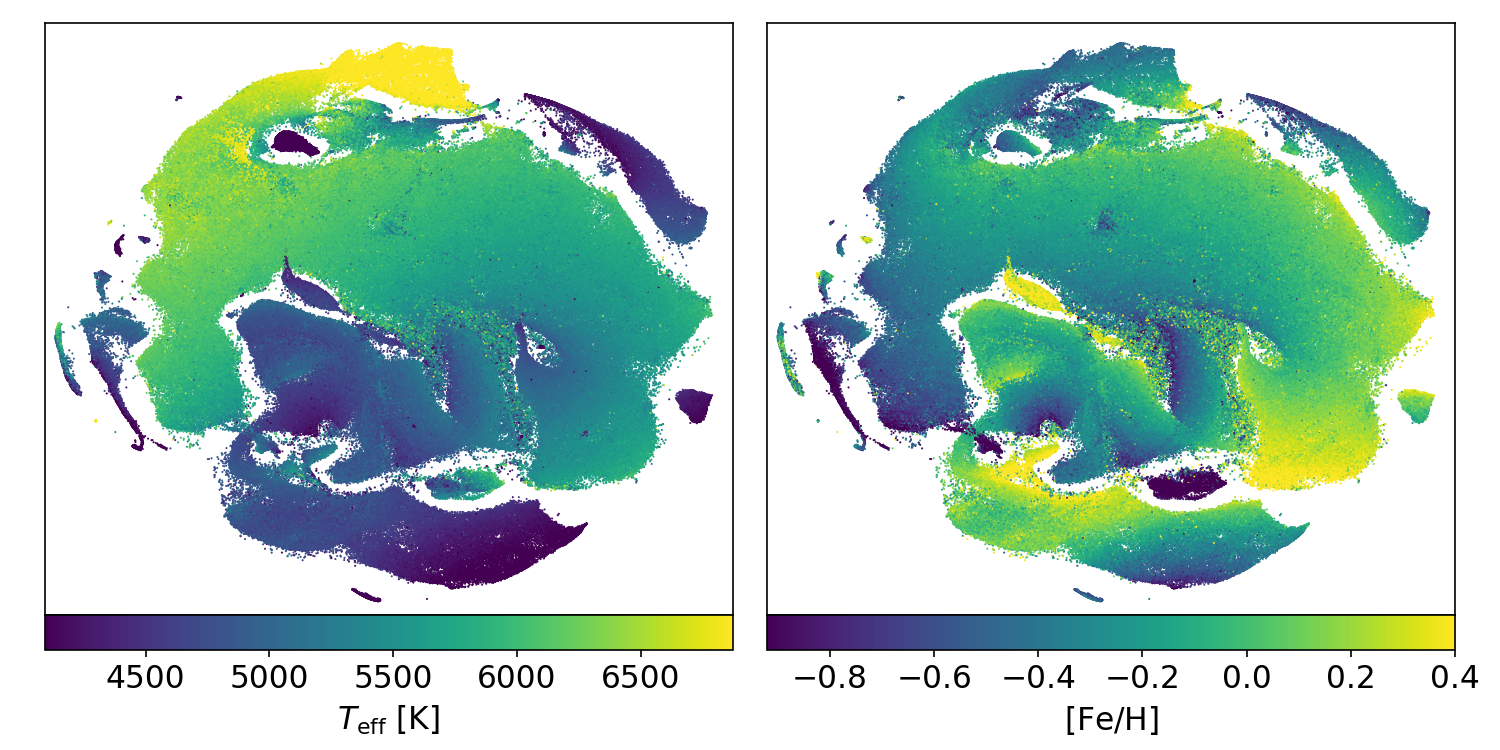
\includegraphics[width=0.95\textwidth]{tsne_params_notitle.png}
	\caption{Spatial distribution of all available measurements of \Teff\ (left panel) and \Feh\ (right panel) as determined by \TC. Dots, representing analysed spectra in the t-SNE projection, are colour coded by their parameter values. Colours and their corresponding values are explained by a colourbar under the graph.}
	\label{fig:tsne_teff_feh}
\end{figure*}

\begin{figure*}
	\centering
	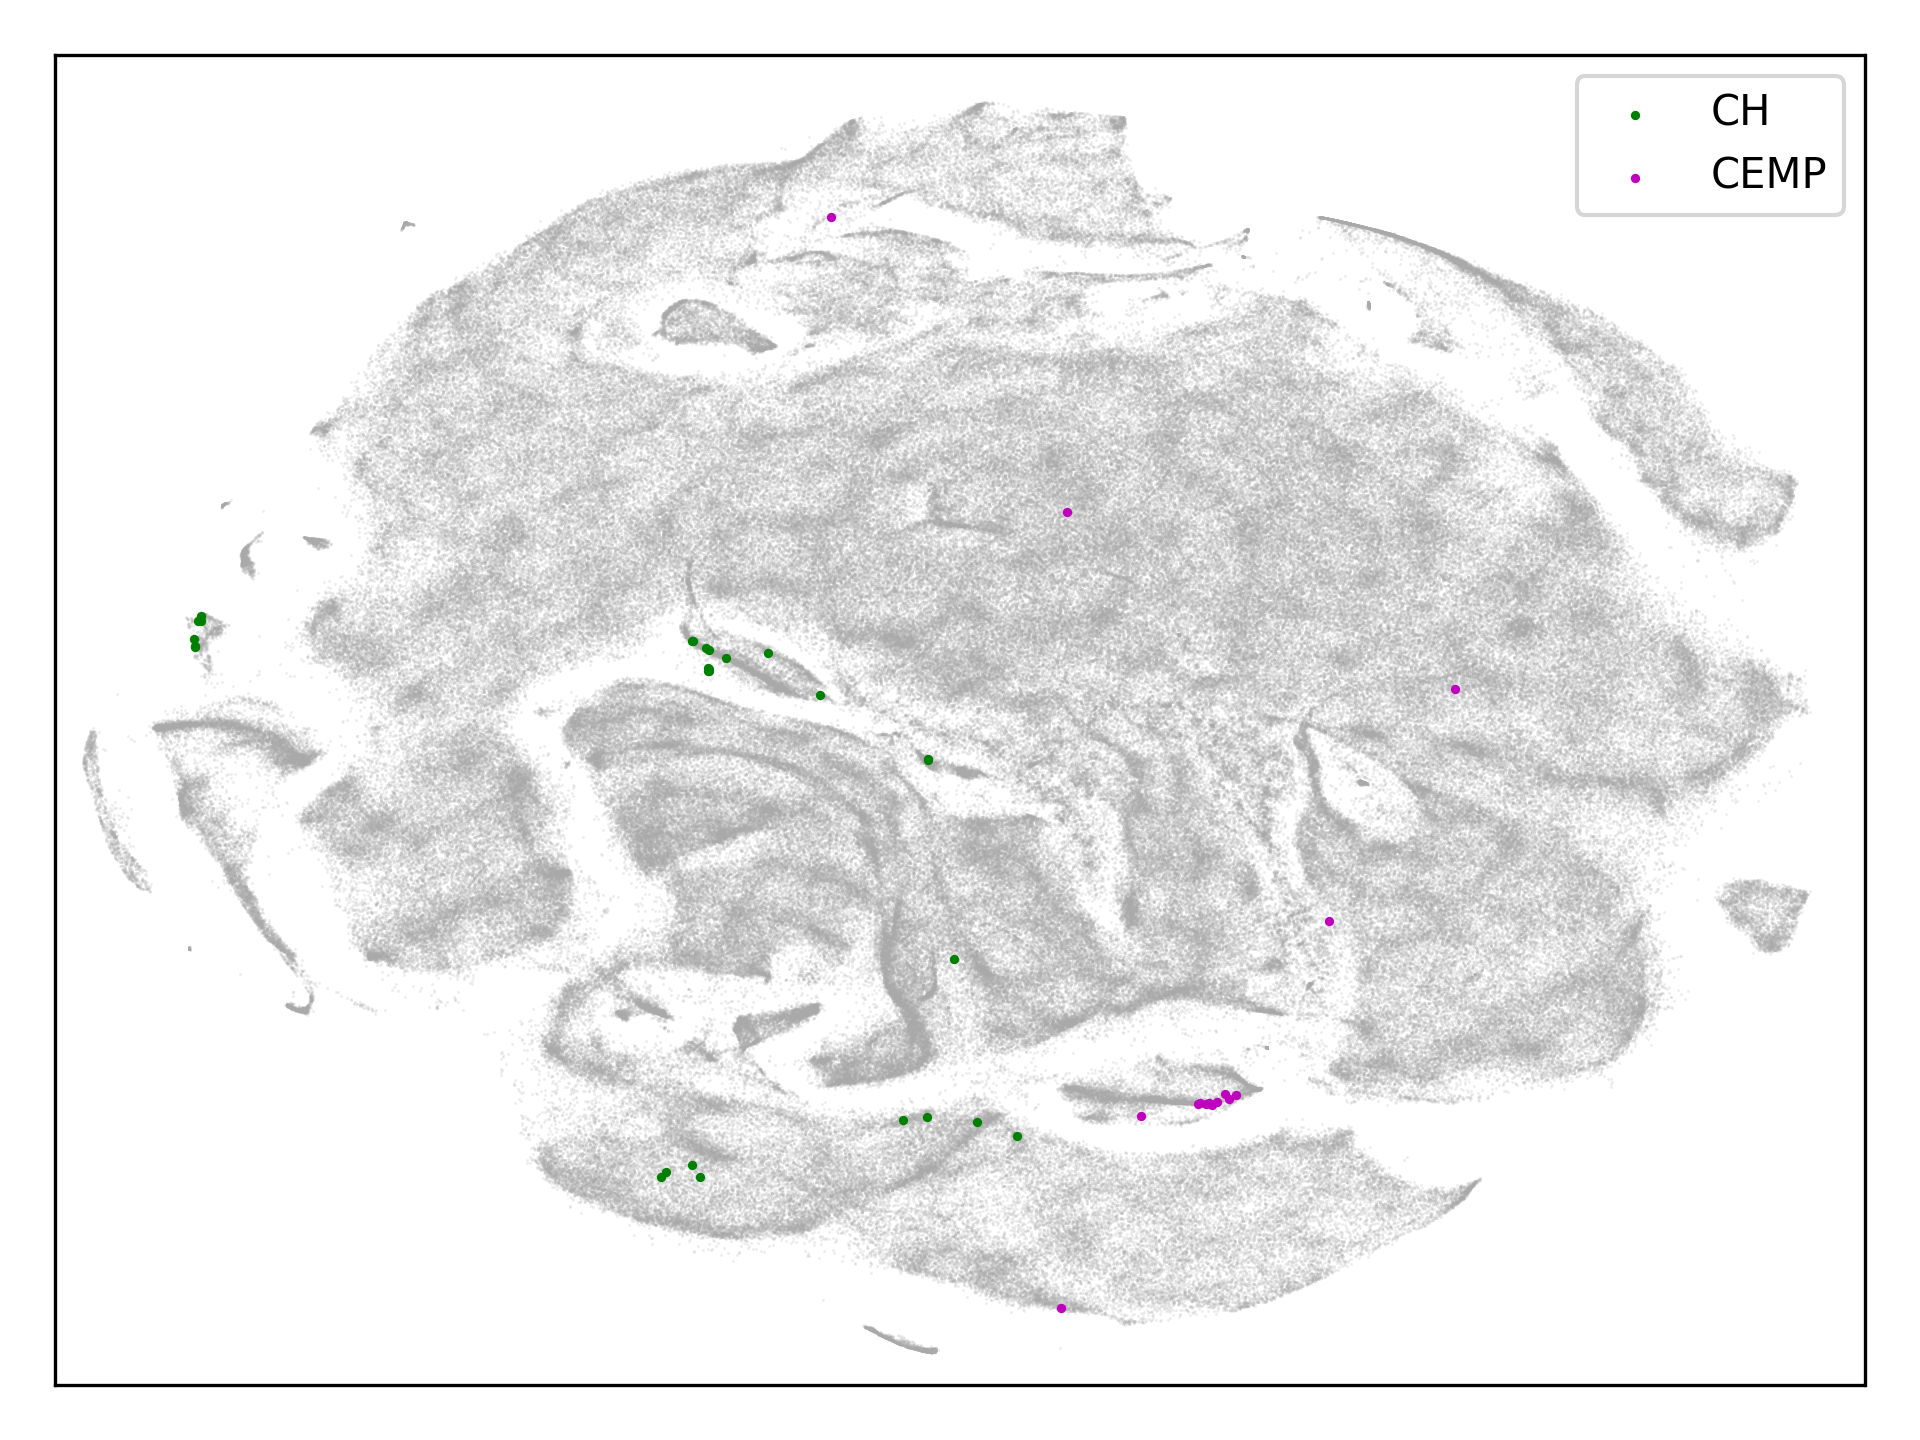
\includegraphics[width=0.95\textwidth]{tsne_refpapers.png}
	\caption{t-SNE projection with marked known carbon-enhanced and CEMP objects from multiple different catalogues found in the literature that are also part of our analysed set of spectra.}
	\label{fig:tsne_ref_ch}
\end{figure*}

\begin{figure*}
	\centering
	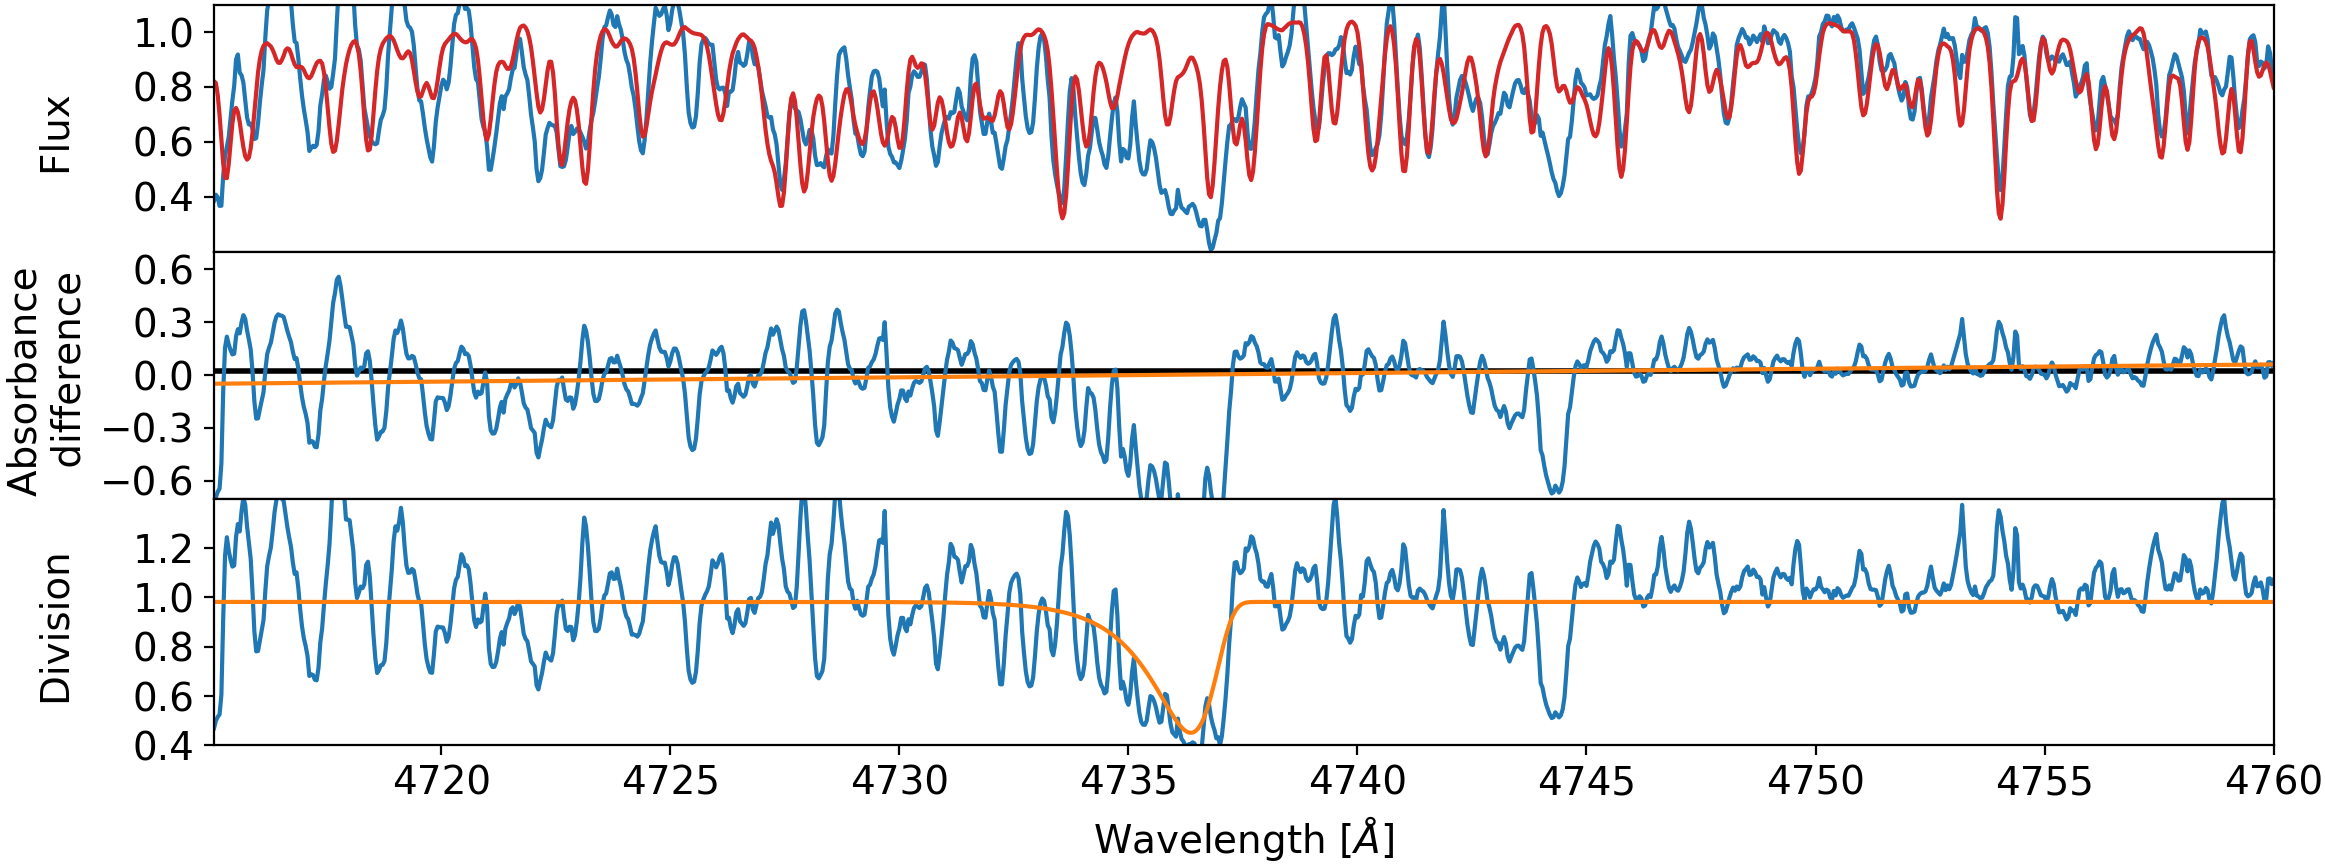
\includegraphics[width=\textwidth]{rich_160515003401143.png}
	\caption{Equivalent plot as in the Figure \ref{fig:carbon_example} but presenting an example of a metal-rich star with multiple strong Swan features around 4737 and 4745 \AA. Presented star has a 2MASS identifier J13121354-3533120 and is known Galactic carbon star \citep{2001BaltA..10....1A}.}
	\label{fig:carbon_example2}
\end{figure*}

\begin{figure*}
	\centering
	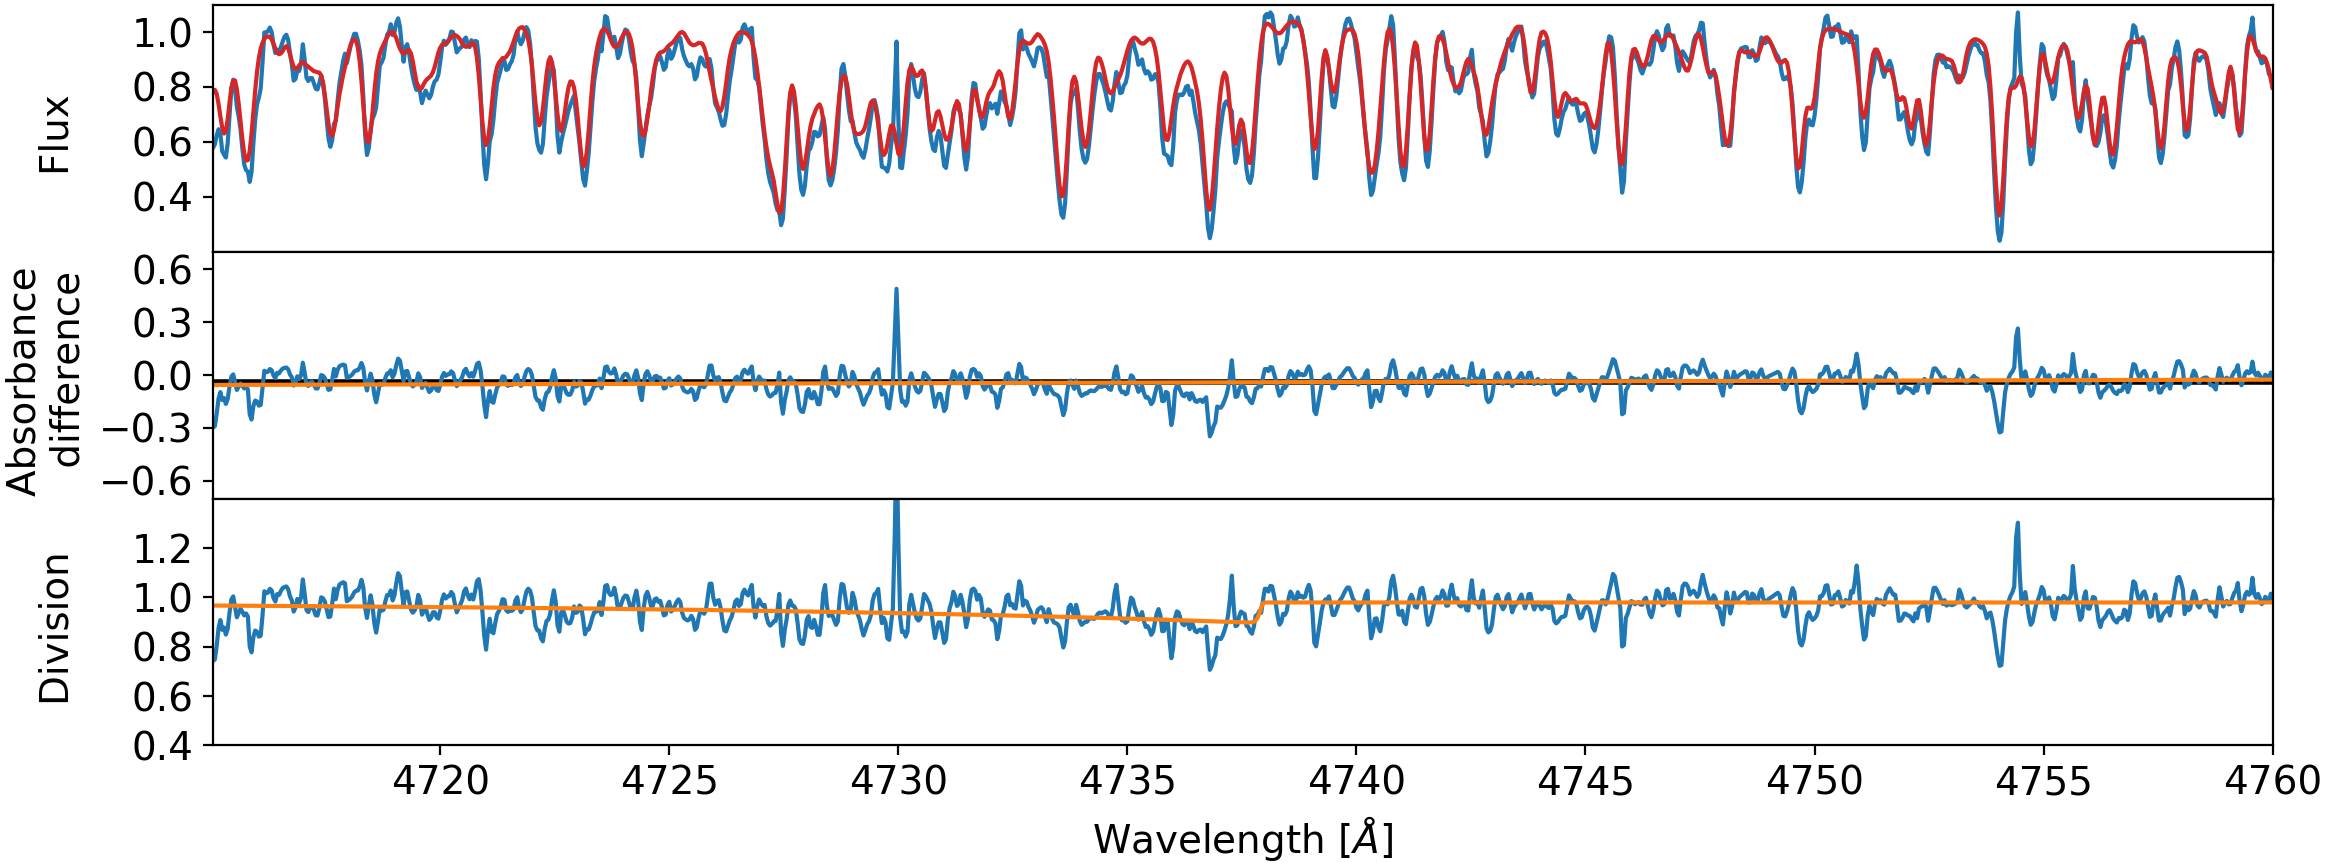
\includegraphics[width=\textwidth]{last_170515005101173.png}
	\caption{Equivalent plot as in the Figure \ref{fig:carbon_example} showing the last of 400 spectra, ordered by their degree of carbon enhancement, selected by the supervised methodology.}
	\label{fig:carbon_last_supervised}
\end{figure*}

\newpage

\begin{figure*}
	\centering
	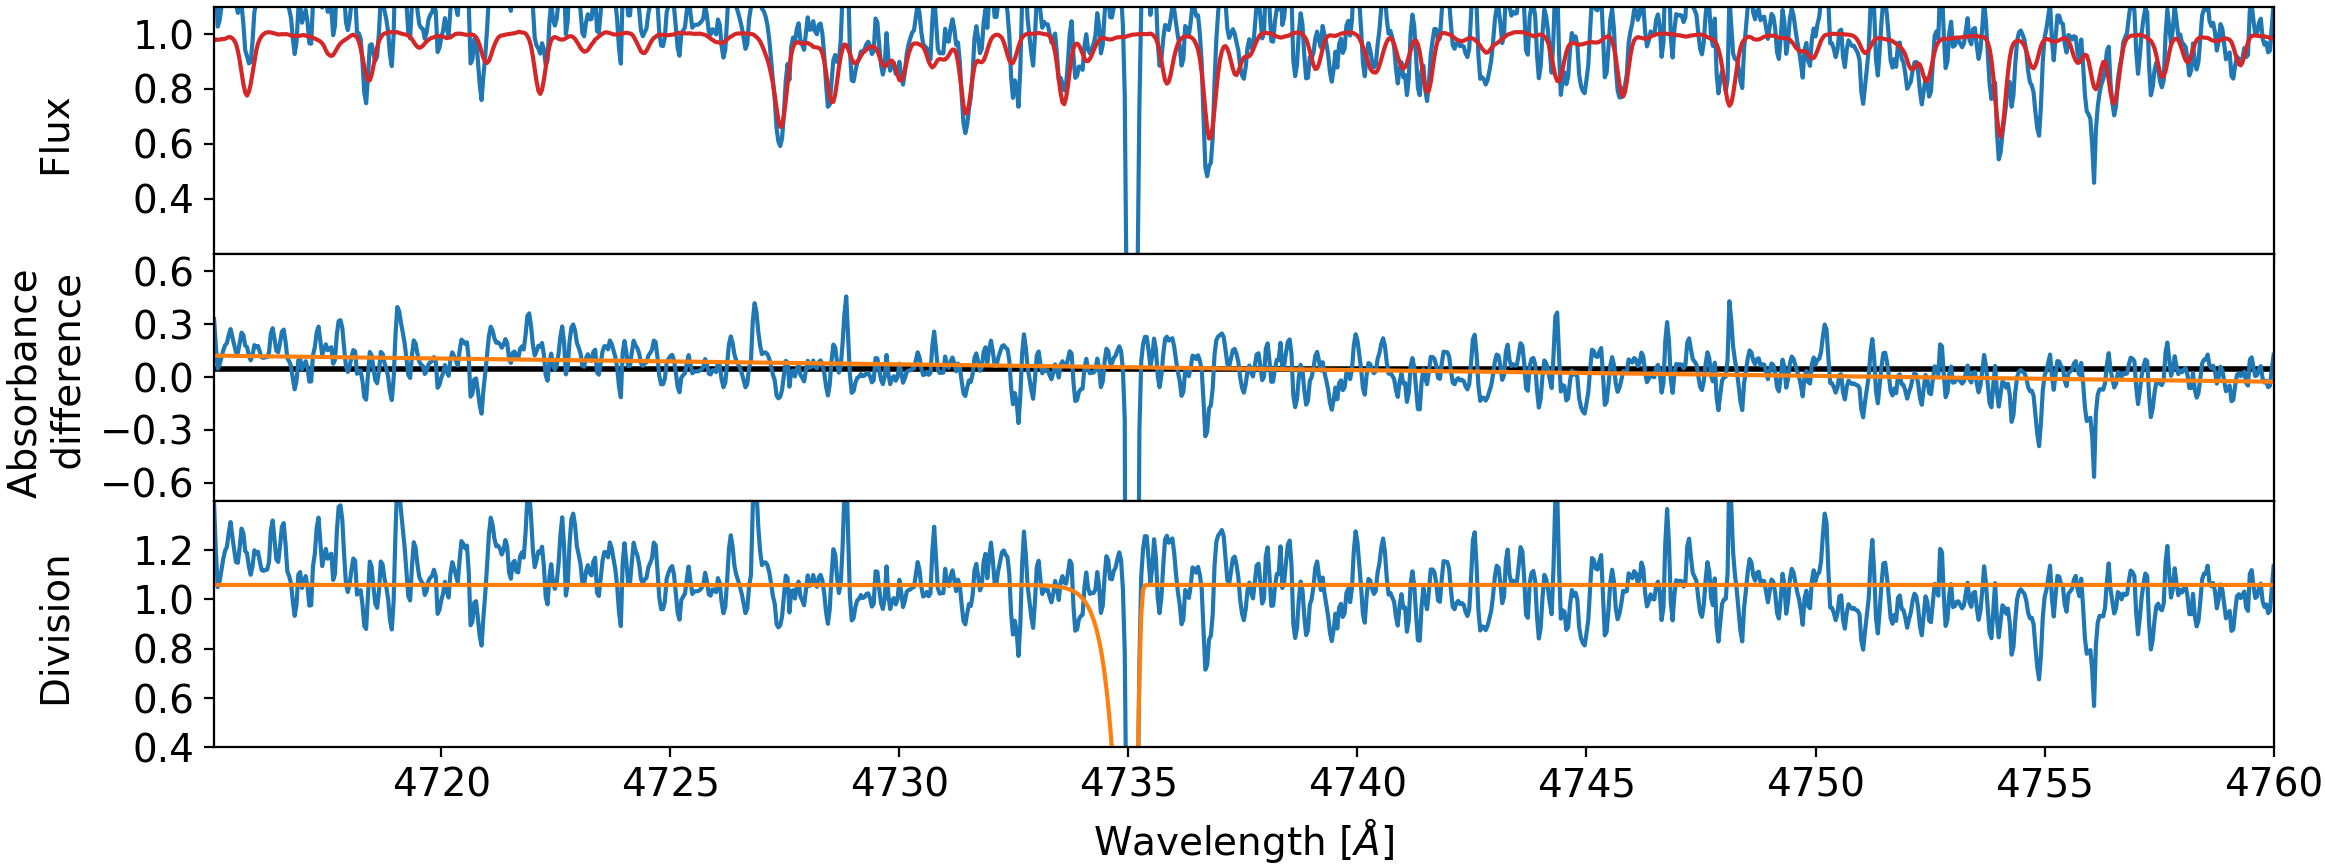
\includegraphics[width=\textwidth]{bad_fit1_150902002901051.png}
	\caption{Equivalent plot as in the Figure \ref{fig:carbon_example} but representing grossly over exaggerated carbon enhancement by a fit that describes a reduction problem (a cosmic ray in a subtracted sky spectrum).}
	\label{fig:bad_fit1}
\end{figure*}

\begin{figure*}
	\centering
	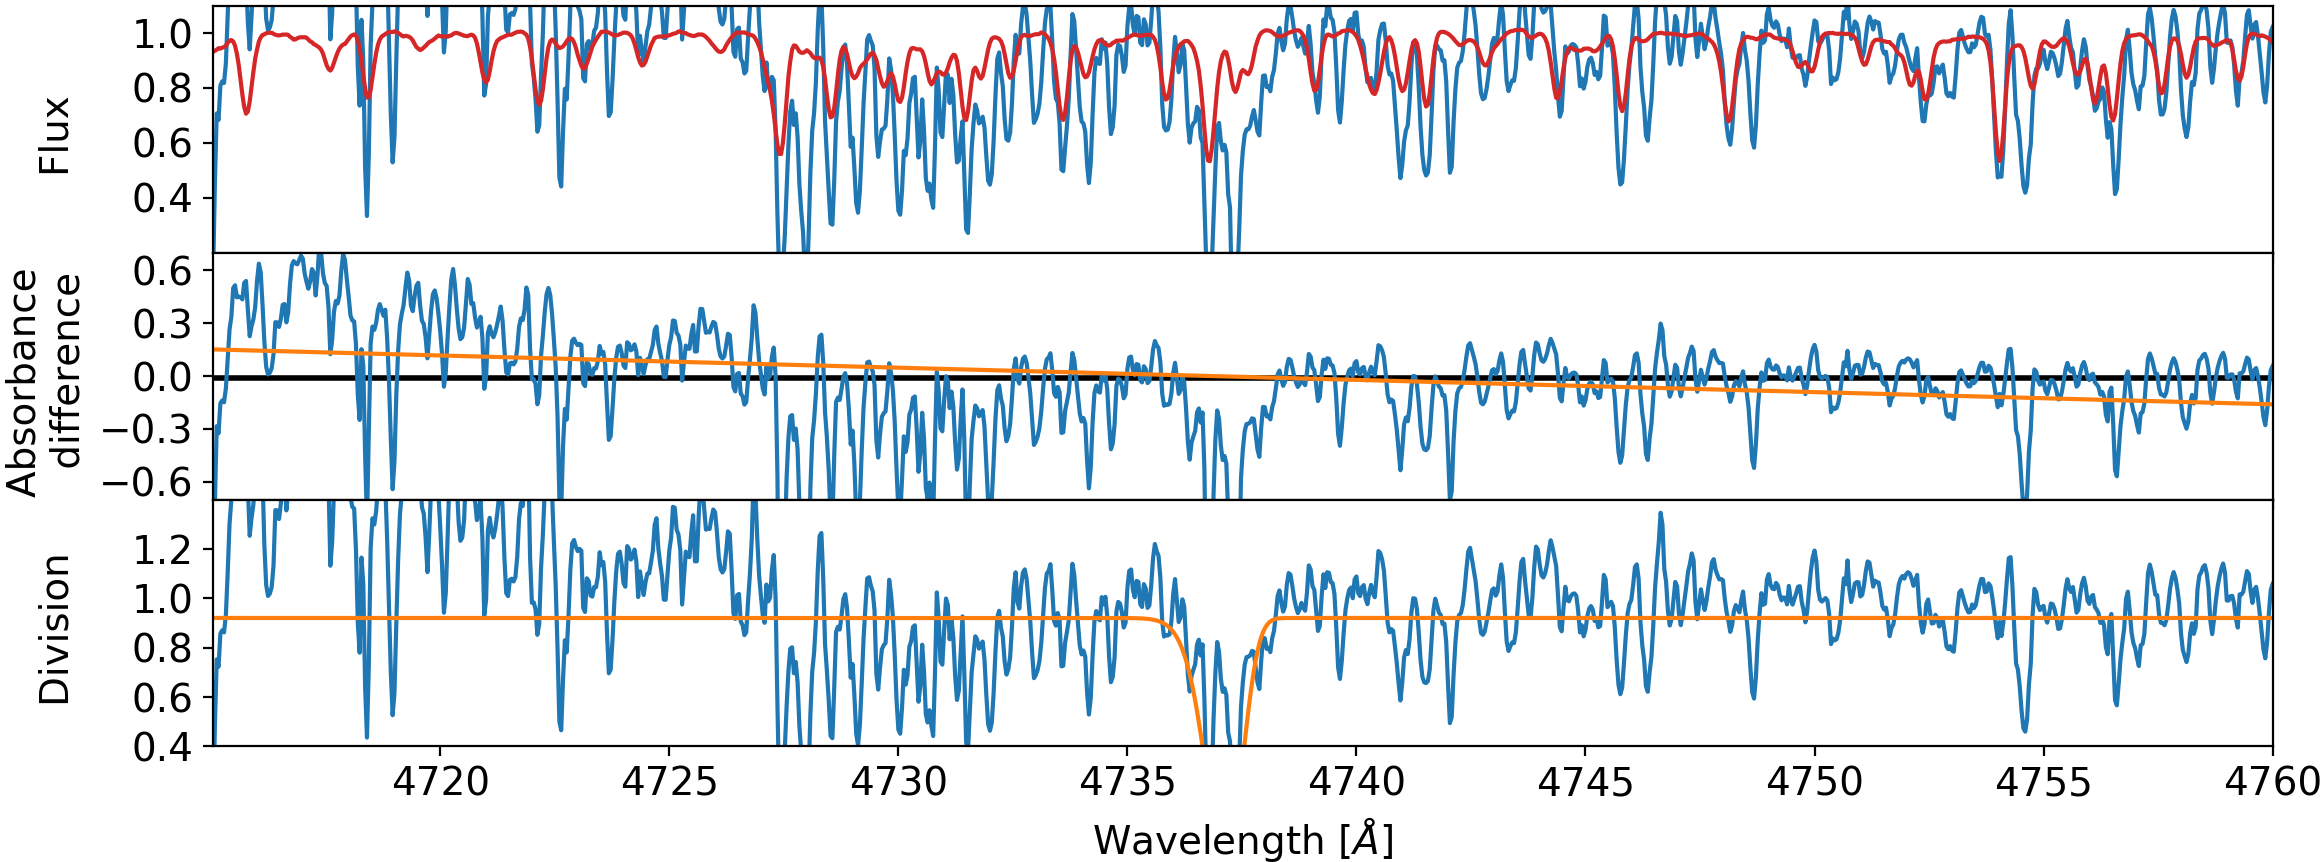
\includegraphics[width=\textwidth]{bad_fit2_150603001801056.png}
	\caption{Equivalent plot as in the Figure \ref{fig:carbon_example} but representing a fit to absorption lines of a double-lined spectroscopic binary. Final fit is not skewed as would be expected in the case of carbon enhancement.}
	\label{fig:bad_fit2}
\end{figure*}

\begin{figure*}
	\centering
	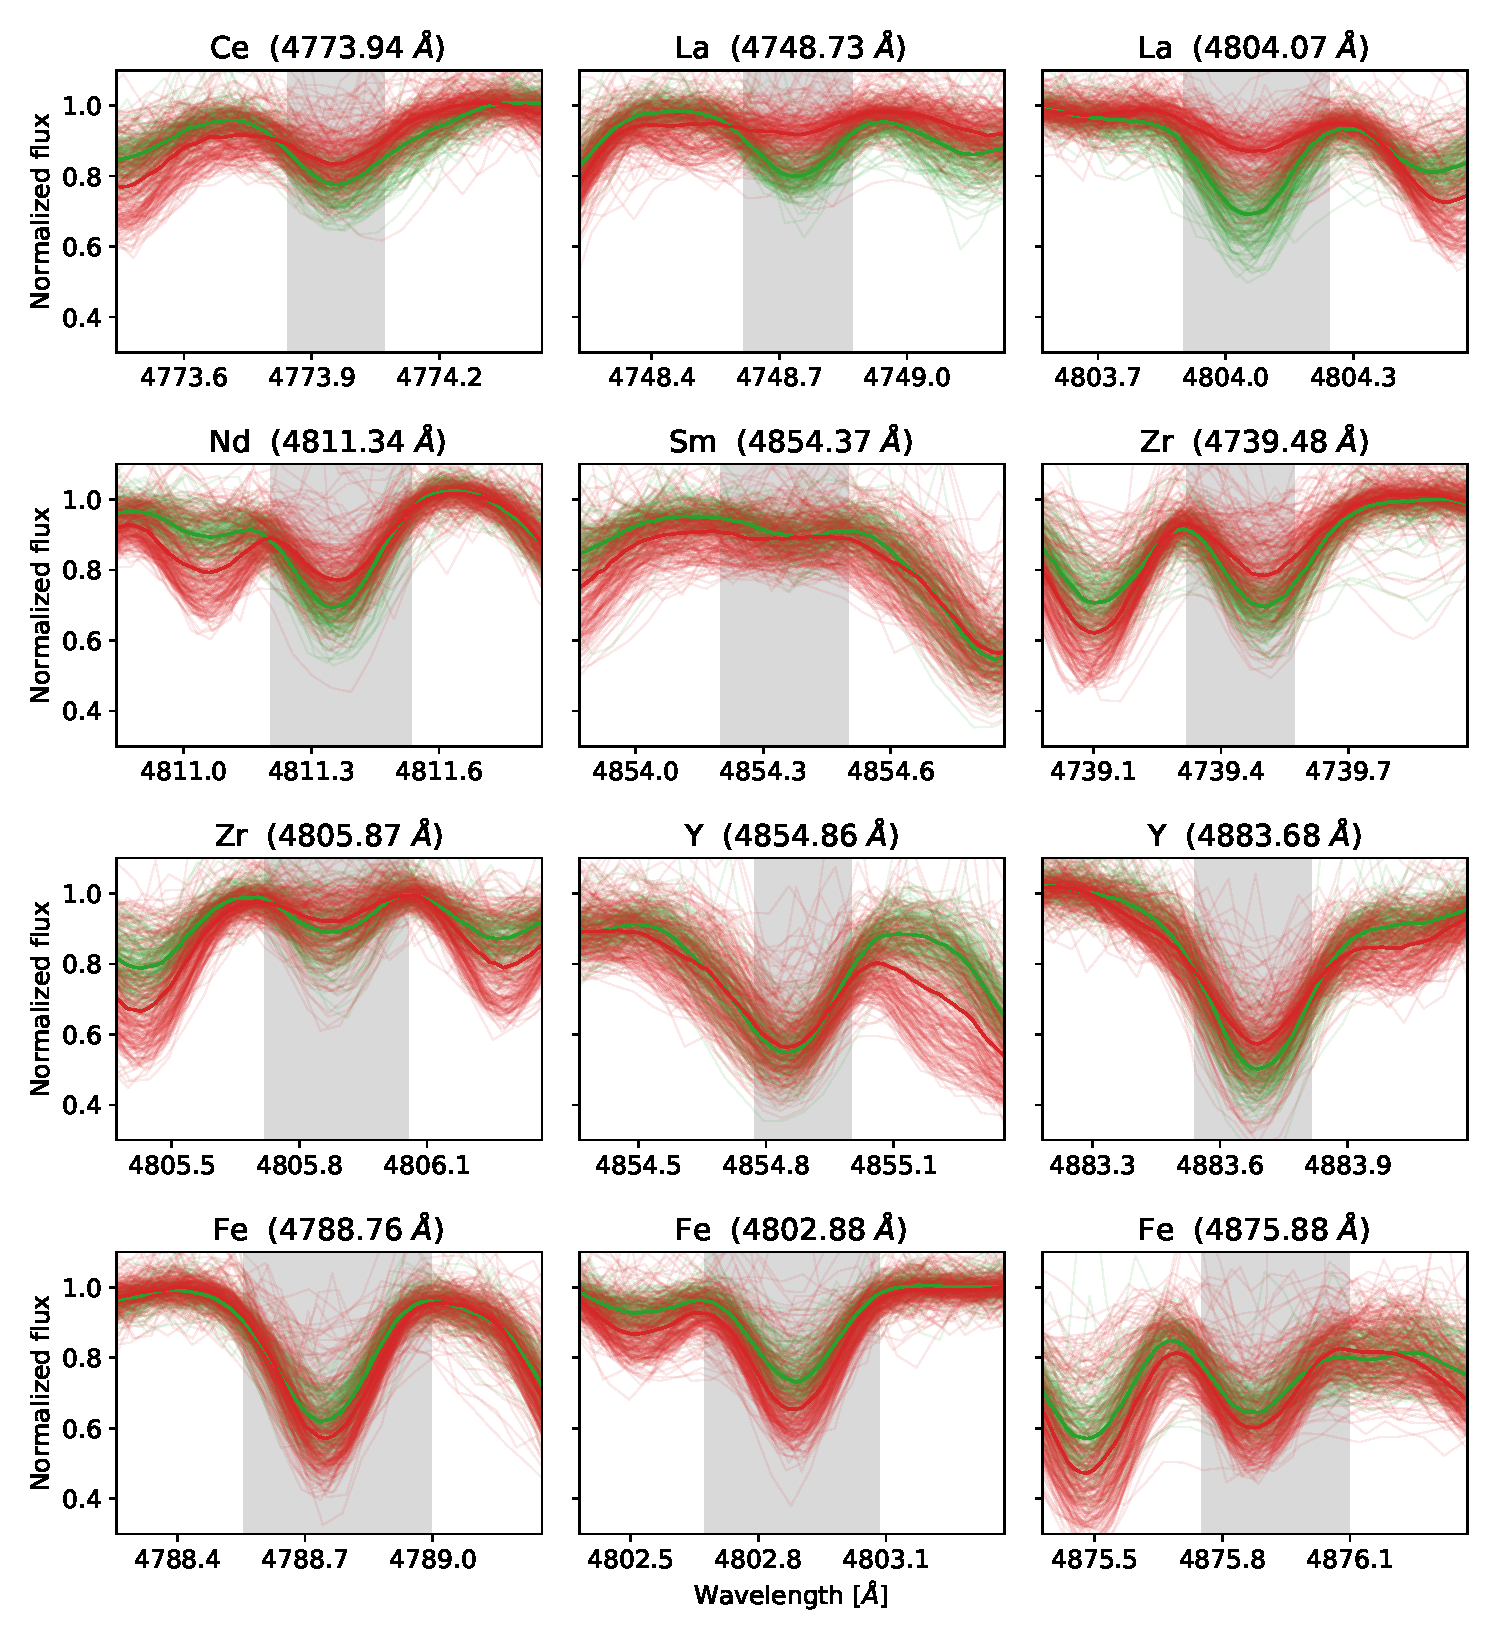
\includegraphics[width=\textwidth]{sprocess_spectra.pdf}
	\caption{Spectral subset around the absorption features in the blue arm that were used to determine abundances of Fe and s-process elements. Same colour coding is used as in Figure \ref{fig:sprocess_hist}. Spectra inside the t-SNE determined clump are shown in red, and outside it in green. Median of all spectra is shown with a bold line of the same colour. The shaded area gives the wavelength range considered in the computation of abundances.}
	\label{fig:sprocess_spectrum}
\end{figure*}

\begin{figure}
	\centering
	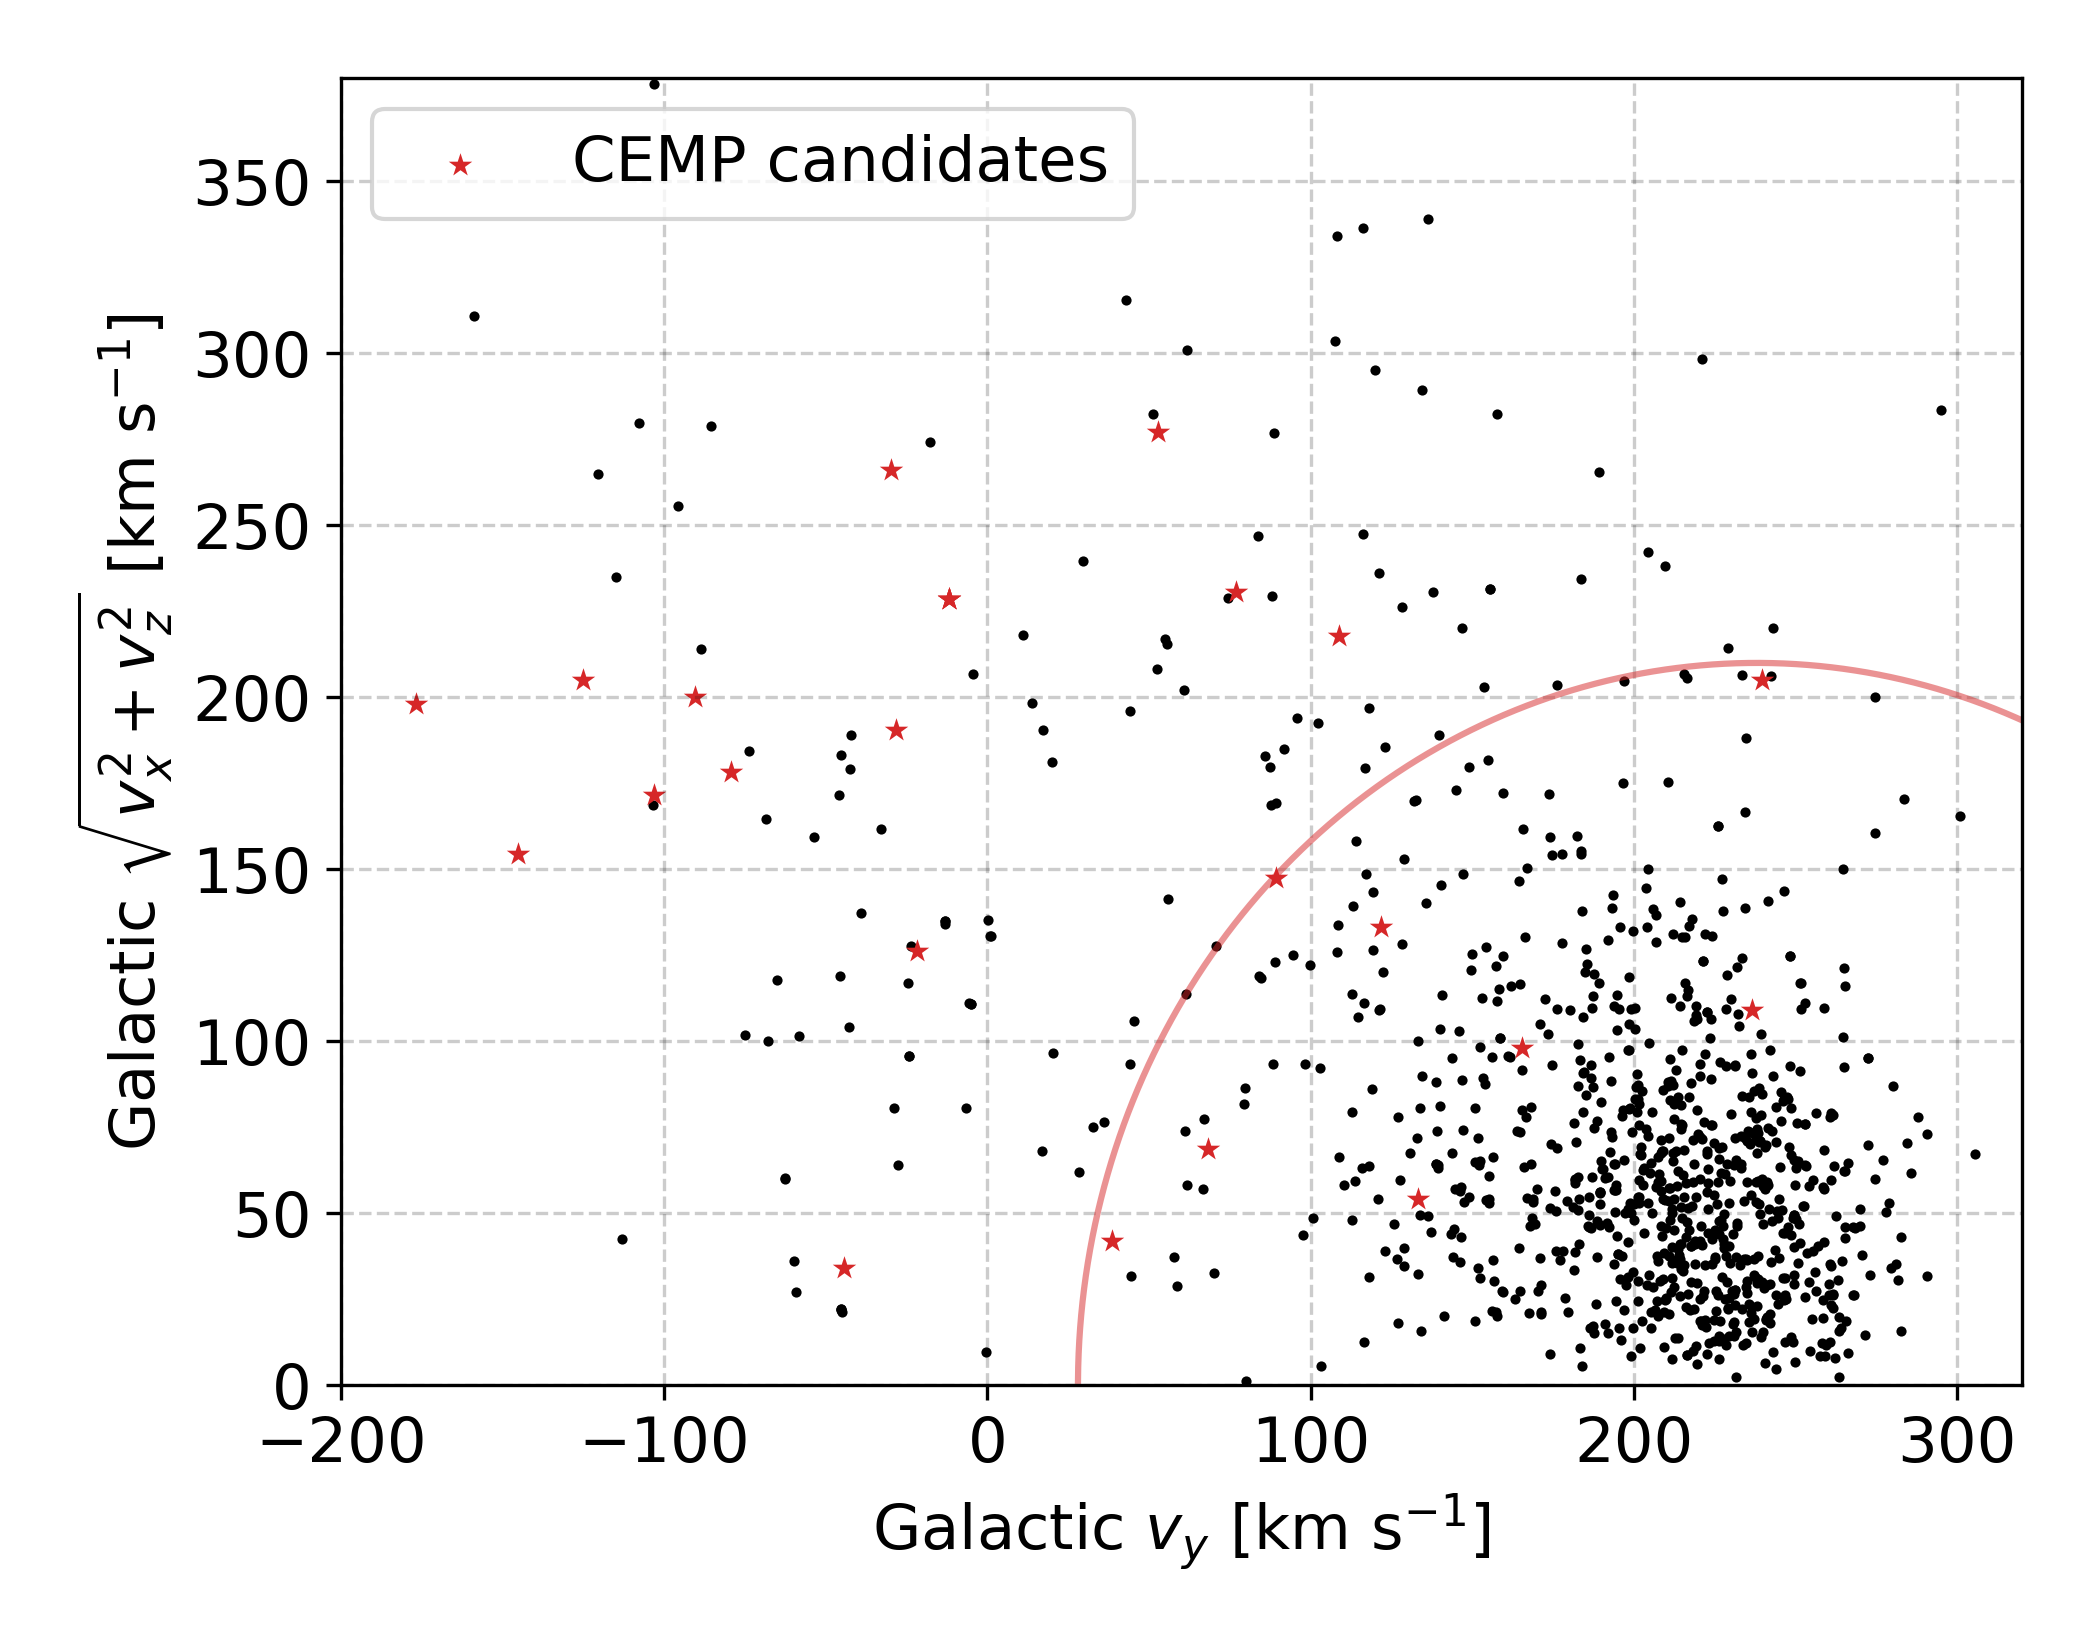
\includegraphics[width=\columnwidth]{carbon_orbits_vy_vxvz.png}
	\caption{Toomre diagram used to identify possible local halo stars among our detected carbon-enhanced stars, especially CEMP candidates. Halo stars in this diagram are located above the red circular line, satisfying the velocity condition $\left|\mathbf{v} - \mathbf{v_{LSR}} \right|$~>~210~\kms\ \citep[the threshold taken from ][]{2018ApJ...860L..11K}. CEMP candidates are marked with star symbols.}
	\label{fig:orbits_vxvyvz}
\end{figure}


\chapter{Conclusions}
The fast increase in observational data seen in the last decade with the introduction of new and improved astronomical observational facilities requires new approaches to the exploration of acquired data. The old mentally of exact and painstaking analysis of individual objects had to be changed in order to grasp the full potential of large observational sets. On the other hand, large amounts of data and complex observational scenarios also lead to more complicated data reduction and analysis pipelines. As it is impossible to look through all acquired data and consider all variables, many computer algorithms have over the years been developed to help with those tasks. Of them, the most trending and occasionally misused are numerous machine learning procedures of classification, clustering, and regression.

In this thesis, we used some of the available machine learning tools to explore large astronomical datasets, mainly collected as part of the \Gh\ and \G\ large sky surveys. The data of those surveys were, when needed, supplemented with results of other spectroscopic and photometric surveys. This merger gave us additional information by observing a broader wavelength range and an increase in temporal coverage of variabilities by combing similar data sets.

The body of this thesis focuses on exploring different types of stars. Usually, the stars are generally separated into two broad groups: normal and peculiar. The first term describes the majority of the stars that are happily living through the longest period of their lifetime. Being non-problematic, they are easily modelled and preferred for chemical analyses such as our exploration of open stellar clusters and their surrounding. During the analysis, we explored the possibility of chemical differentiation between chemical signatures of cluster members, possible past members and surrounding stars. Separation into given components for 11 open clusters was based on kinematic vectors defined by \G\ observations. The \Gh\ survey supplied the chemical signature for a subset of stars. The analysis of open clusters in our dataset showed that they are not chemically as homogeneous as theory says and as much as we would like. Not knowing the origin of this discrepancy, we shifted to the differential chemical analysis that takes out the identified trends and compares only chemical signatures of stars with the same stellar parameters, most commonly effective temperature. The results show that uncertainties of the determined abundances and their scatter limit chemical separability between an open cluster and field stars as the majority have very comparable signatures. We showed that inclusion of kinematic information helps with the delineation as it was more likely that potentially ejected stars were chemically tagged to the cluster than remaining field stars.

The second large groups of stars that are not wanted in the above-described analyses are peculiar stars. The term is inclusive and depends on the scientific question in hand and observed wavelength region. In our case, the definition includes spectroscopically detectable classes such as interacting stars, multiple stellar systems, stars in temporally short-lived evolutionary stages and spectra with unexpected chemical compositions. Our selection of all peculiar classes depended on the comparison between normal-looking spectra and observed spectra. The modelling of normal spectra was done in multiple different ways: by averaging spectra with similar parameters, running observed spectra trough a neural network autoencoder and modelling using spectrum generative approach \TC. The direct comparison gave us a difference between spectral modelling and reality. When we were looking at the specific wavelength regions, we uncovered spectra with pronounced molecular absorption bands of C$_2$ - stars that are carbon-rich and spectra with expressed hydrogen, [NII], and [SII] emission lines. As the emission lines are results of different ongoing processes on a star and around it, we tried to delineate them on chromospheric and nebular contributions using the derived line parameters such as position, strength and shape. Combination of normal single star spectra can also be used for the spectral disentanglement of multiple stellar systems. Our methodology was used to describe over-luminous stars whose spectra did not show signs of multiple stars in a system. Therefore we assumed that comprising stars in the system must be orbiting on wide orbits. By combining photometric and spectroscopic single star models, we were able to reproduce the observable quantities and confirm the existence of triple systems with near-identical stars. Orbits of such proposed systems were also modelled to confirm that their configuration is consistent with observational limitations.

All tabulated results presented in this thesis are also published as freely available catalogues on the astronomical online database collection VizieR and directly from the publishers' website. The compiled catalogues could serve as a starting point for many additional research that deals with the exact physics behind identified peculiar stars and their spectra. Some of the possibilities for future studies were already given in the text and will be considered as potential observing possibilities at the available observing facilities, such as Asiago observatory where we are conducting spectroscopic observations almost every month. Most often, spectroscopic data must be complemented with photometric sets to explore or confirm additional possible physical scenarios behind interesting objects.

The hype of the big data era in astronomy is still to increase as many new telescopes and instruments are currently under development and construction. Their observations are planned to start in the following years. Until then, the \G\ satellite is continuously scanning our sky in order to bring us the most precise distances and movements for billions of stars that we are all warning for. The next grander data release is still at least a year away, but everyone is already questioning how much more can it do for science in the field of galactic archaeology. In our case, the updated distances could completely change the membership, shape and structure of open clusters and reclassify exciting possible triple stars to dull single free-floating stars because of their parallactic uncertainty. Until then, we have to double-check our applied quality filters and trust in the data and parameters currently disposable at our hands.


%------------------------------------------------------------------------------------
%       LITERATURA
%------------------------------------------------------------------------------------

\cleardoublepage\phantomsection
\renewcommand\bibname{Bibliography}
\addcontentsline{toc}{chapter}{Bibliography}
\bibliographystyle{apsrev4-2-fmf-eng}
\bibliography{Bibliografija-eng}


%-------------------------------------------------------------------------------------
%       DODATKI
%------------------------------------------------------------------------------------

\cleardoublepage\phantomsection
\renewcommand\appendixname{Appendix}
\begin{appendices}

\chapter{Naslov prvega dodatka}
    

\end{appendices}


\cleardoublepage\phantomsection
\addcontentsline{toc}{chapter}{Razširjeni povzetek v slovenskem jeziku}
\chapter*{Razširjeni povzetek v slovenskem jeziku}
\markboth{Razširjeni povzetek v slovenskem jeziku}{}

\foreignlanguage{slovene}{  % slovenski delilni vzorci
Razširjeni povzetek v slovenskem jeziku naj bo dolg vsaj 10 strani. 
Vključuje naj tudi slike, tabele in enačbe, ki so nujne za razumevanje besedila povzetka.
}

%---------------------------------------------------------------------------------
%       KAZALO (NEOBVEZNO)
%--------------------------------------------------------------------------------

\cleardoublepage
\printindex

%------------------------------------------------------------------------------
%       SEZNAM OBJAV (CE OBSTAJAJO)
%-----------------------------------------------------------------------------

\cleardoublepage\phantomsection
\addcontentsline{toc}{chapter}{List of publications related to this doctoral thesis}
\chapter*{List of publications related to this doctoral thesis}


\begin{enumerate}

\item
Ivan Kuščer,
\textit{Multiple small-angle scattering of light},
Prog. Nucl. Energy
\textbf{34},
355 (1999).

\end{enumerate}


\end{document}